\documentclass[12pt,a4paper,oneside]{book}
\usepackage[utf8]{vietnam}
\usepackage{amsmath, amsfonts, amssymb, graphicx, mathrsfs}
\usepackage{enumerate, boxedminipage, multicol, etoolbox}
\usepackage{tkz-euclide}
\usepackage{tikz-3dplot}
\usepackage{tikz,tkz-tab}
\usetikzlibrary{tikzmark}
\usetikzlibrary{shapes.geometric,arrows,calc,intersections,angles,patterns,snakes}
\usetikzlibrary{shadows}
%\usetkzobj{all}
%\usepackage{pgfplots}
%\usepgfplotslibrary{fillbetween}
%\pgfplotsset{compat=1.9}
%\usepackage[top=2cm, bottom=2.5cm, left=1.5cm, right=1.5cm] {geometry}
\usepackage[hidelinks,unicode]{hyperref}
\usepackage{currfile}
\usepackage{float}
%Gói căn lề giấy.
\usepackage[top=2cm, bottom=2cm, left=1.5cm, right=1.5cm]{geometry}
\usepackage{lilyglyphs}%vẽ icon
\usepackage{twemojis} 
%Xoá thụt đầu dòng. 
\setlength\parindent{0pt}
\renewcommand{\baselinestretch}{1.2}


%Gói màu sắc.
%\usepackage[dvipsnames]{xcolor}

%Định nghĩa màu.
\definecolor{mauChuDao}{HTML}{1B3D9F}
\definecolor{cqcqcq}{rgb}{0.75,0.75,0.75}
\definecolor{ocre}{RGB}{24,190,250}
\definecolor{ffqqqq}{rgb}{1.,0.,0.}
\definecolor{qqqqff}{rgb}{0.,0.,1.}
\definecolor{ffffff}{rgb}{1.,1.,1.}
%Gói Tikz.
\usepackage{tikz, tkz-tab, tkz-euclide}
\usetikzlibrary{calc, patterns, shadings, angles, intersections, shapes, quotes, trees}

%Gói ex_test.
%\usepackage[dethi]{ex_test}
%\usepackage[loigiai]{ex_test}
\usepackage[book]{ex_test}
\renewcommand{\loigiaiEX}{{\color{mauChuDao}\faKey~Đáp án}}

%Tạo các môi trường mới.
\usepackage[skins,breakable]{tcolorbox}
\usepackage[explicit,calcwidth]{titlesec}
\usepackage{titletoc}
\usepackage{varwidth}
\tcbuselibrary{raster}
\setcounter{secnumdepth}{4}
\setcounter{tocdepth}{1}

%========= Công thức toán =========%
\everymath{\displaystyle}
%Dấu hệ hoặc.
\newcommand{\hoac}[1]
{
	\left[\begin{aligned}#1\end{aligned}\right.
}
%Dấu hệ và.
\newcommand{\heva}[1]
{
	\left\{\begin{aligned}#1\end{aligned}\right.
}
%==================================%

%=======Tùy biến môi trường =======%
\makeatletter
%%%%%%%%%%%%%%%%%%%%%%%%%%%%%%%%
%Tùy chỉnh Mục lục
\usepackage{ifoddpage}
\titleformat{name=\chapter,numberless}[display]
{\normalfont\huge\bfseries}
{}
{-1cm}
{%
	\begin{tikzpicture}[remember picture, overlay]%
		\draw[fill=mauChuDao, rounded corners=15pt] (12.5,-.75) rectangle (20,1.3);%
		\draw (13.5,0.2) node [right]{\color{white}\fontsize{25pt}{1pt}\fontfamily{qag}\selectfont\bfseries\MakeUppercase{#1}};%
	\end{tikzpicture}
}
[
\vspace{1cm}
]
%%%%%%%%%%%%%%%%%%%%%%%%%%%%%
%%%%%%%%%%%%%%%%%%%%%%%%%%%%%%

\renewcommand*\l@part[2]{%
	\ifnum \c@tocdepth >-2\relax
	\addpenalty{-\@highpenalty}%
	\addvspace{2.25em \@plus\p@}%
	\setlength\@tempdima{3em}%
	\begingroup
	\parindent \z@ \rightskip \@pnumwidth
	\parfillskip -\@pnumwidth
	{\leavevmode
		\normalsize \bfseries #1\dotfill
		\hb@xt@\@pnumwidth{\hss #2%
			\kern-\p@\kern\p@}}\par
	\nobreak
	\global\@nobreaktrue
	\everypar{\global\@nobreakfalse\everypar{}}%
	\endgroup
	\fi}
%Title chapter
\renewcommand*\l@chapter[2]{%
	\ifnum \c@tocdepth >\m@ne
	\addpenalty{-\@highpenalty}%
	\vskip 1.0em \@plus\p@
	\setlength\@tempdima{1.5em}%
	\begingroup
	\parindent \z@ \rightskip \@pnumwidth
	\parfillskip -\@pnumwidth
	\leavevmode \bfseries
	\advance\leftskip\@tempdima
	\hskip -\leftskip
	\hspace*{0.5cm}CHƯƠNG #1\nobreak\dotfill
	\nobreak\hb@xt@\@pnumwidth{\hss #2%
		\kern-\p@\kern\p@}\par
	\penalty\@highpenalty
	\endgroup
	\fi}
%Title section
\renewcommand*\l@section[2]{%
	\ifnum \c@tocdepth >\m@ne
	\addpenalty{-\@highpenalty}%
	\vskip 0.5em \@plus\p@
	\setlength\@tempdima{1.5em}%
	\begingroup
	\parindent \z@ \rightskip \@pnumwidth
	\parfillskip -\@pnumwidth
	\leavevmode \footnotesize
	\advance\leftskip\@tempdima
	\hskip -\leftskip
	\hspace*{1cm}#1\nobreak\dotfill
	\nobreak\hb@xt@\@pnumwidth{\hss #2%
		\kern-\p@\kern\p@}\par
	\penalty\@highpenalty
	\endgroup
	\fi}

%----------------------------------%
%Môi trường Phần
\renewcommand{\thepart}{\arabic{part}}
\titleformat{\part}
{
	\thispagestyle{fancy}\filcenter\color{mauChuDao}\bfseries
}
{		
	\definecolor{mauPhan}{HTML}{FF0066}
	
\begin{tikzpicture}
		\node at (0,0){\fontsize{28pt}{1pt}\selectfont\MakeUppercase\partname};
		\node[shape = star, fill =mauChuDao, inner sep = 5pt] at (0,0)[shift = {(0,-4)}] {\textcolor{white}{\fontsize{70pt}{1pt}\selectfont \thepart}};
	\end{tikzpicture}
}
{0 cm}
{
	\vskip 5pt\titlerule[2.5pt]\vskip 1.5pt\titlerule[1pt]\vskip 5pt 
	\fontsize{25pt}{10pt}\selectfont\MakeUppercase{#1}
}
%----------------------------------%
%Môi trường Chương
\renewcommand{\chapter}
{
	\if@openright\cleardoublepage\else\clearpage\fi
	\global\@topnum\z@
	\@afterindentfalse
	\secdef\@chapter\@schapter
}
\titleformat{\chapter}
{}
{}
{0em}
{
	\begin{tikzpicture}
		\node (base){\color{mauChuDao}\bfseries\fontsize{18}{0}\selectfont \faGripfire CHƯƠNG\faGripfire};
		\node[draw=mauChuDao,circle,line width=2pt] (num) at ([yshift=-0.9cm]base.-90){\color{mauChuDao}\fontsize{30}{0}\selectfont\thechapter};
		\node at ([yshift=-0.3cm]num.-90){\color{mauChuDao}\faGg\faGg\faGg};
		\draw[double, double distance=0.1cm, line width=2pt, mauChuDao] ([shift={(1.8,-0.5)}]num.south east)--++(\textwidth-5cm,0);
		\node[text width={\textwidth - 5cm}, right] (content) at ([shift={(1.3,0)}]num.0){\color{mauChuDao}\bfseries\fontsize{15pt}{0pt}\selectfont\MakeUppercase{#1}};
	\end{tikzpicture}
}
[   
\setcounter{dn}{0}
\setcounter{dl}{0}
\setcounter{hq}{0}
]
\titlespacing{\chapter}{0cm}{0cm}{0.5cm}[0cm]
%----------------------------------%
%Môi trường Bài
\renewcommand*{\thesection}{\arabic{section}}
\titleformat{\section}
{\centering}
{}
{0pt}
{
	\begin{tikzpicture}
		\node[text width={\textwidth-2cm},text centered] (A){
			\color{mauChuDao}\bfseries\fontsize{15}{0}\selectfont\S\thesection. \MakeUppercase{#1}
		};
	\end{tikzpicture}
}
\titlespacing{\section}{0cm}{1cm}{0cm}[0cm]

%----------------------------------%
%Môi trường Mục
\renewcommand*{\thesubsection}{\Alph{subsection}}
\titleformat{\subsection}
{
	\bfseries
}
{
	\begin{tikzpicture}
		\node[mauChuDao, shape=star, draw, line width = 1pt, inner sep=2pt] (char){\fontsize{15}{0}\selectfont\color{mauChuDao}\bfseries\thesubsection};
		\node[right, text width=\textwidth-2cm] (content) at ([xshift=0.5cm]char.0){\fontsize{13}{0}\selectfont\color{mauChuDao}\bfseries\MakeUppercase{#1}};
	\end{tikzpicture}
}
{0pt}
{}
[
]
\titlespacing{\subsection}{-0.4cm}{0cm}{0cm}[0cm]
%----------------------------------%
%Môi trường mục con.
\renewcommand*{\thesubsubsection}{\arabic{subsubsection}}
\titleformat{\subsubsection}
{
	\bfseries
}
{
	\begin{tikzpicture}
		\node[mauChuDao, shape=circle, draw, fill=mauChuDao, line width = 1pt, inner sep=2pt] (char){\fontsize{12}{0}\selectfont\color{white}\bfseries\thesubsubsection};
		\node[right=0.5cm, text width=\textwidth-2cm] (content) at (char.0){\fontsize{12}{0}\selectfont\color{mauChuDao}\bfseries\MakeUppercase{#1}};
	\end{tikzpicture}
}
{0pt}
{}
[
]
\titlespacing{\subsubsection}{-0.15cm}{0cm}{0cm}[0cm]


%Môi trường Bài tập
\newtheorem{bt}{\bfseries Bài}
%Môi trường Chứng minh.
\theoremstyle{nonumberplain} 
\theoremheaderfont{\bfseries\slshape} 
\theorembodyfont{\normalfont}
\theoremsymbol{\ensuremath{_\blacksquare}} 
\newtheorem{proof}{Chứng minh}
\newcommand{\chm}[1]{\begin{proof}#1\end{proof}}
%----------------------------------%
\makeatother
%==================================%


%==================================%
\newcommand{\tikzHeaderFooter}{
	\begin{tikzpicture}[scale=1, font=\footnotesize, line join=round, line cap=round,>=stealth, overlay, remember picture]
		\def\h{1} %Chiều cao của box
		\coordinate (D) at (current page.east);
		\coordinate (T) at (current page.west);
		\coordinate (B) at (current page.north);
		\coordinate (N) at (current page.south);
		\coordinate (TN) at (current page.south west);
		\coordinate (DN) at (current page.south east);
		\coordinate (TB) at (current page.north west);
		\coordinate (DB) at (current page.north east);
		\coordinate (CT) at (current page.center);
		\fill[mauChuDao] (TB)++(\paperwidth*0.42,-0.5)--++(180:\paperwidth*0.42)--++(-90:\h)--++(0:\paperwidth*0.37)arc(-90:-45:10pt)
		(DB)++(-\paperwidth*0.1,-\h-0.5)--++(0:\paperwidth*0.1)--++(90:\h)--++(180:\paperwidth*0.05) arc (90:135:10pt)
		(TN)++(\paperwidth*0.7,0.5)--++(180:\paperwidth*0.7)--++(90:\h)--++(0:\paperwidth*0.65) arc (90:45:10pt)
		
		;
		\draw[mauChuDao, line width=4pt] (DN)++(0,0.5)--++(180:\paperwidth);
		\draw[mauChuDao, -o, line width=2pt](DB)++(0,-\h-0.5)--++(180:\paperwidth*0.55)
		;
		%		\fill[mauChuDao] (TB)--++(-90:\paperheight/12)..controls +(45:2)..($(DB)+(-90:\paperheight/24)$)--(DB) (DN)--++(90:\paperheight/12)..controls +(225:2)..($(TN)+(90:\paperheight/24)$)--(TN);node[mauChuDao, right]{\bfseries STAR EDUCATION}
		\draw ($(TB)+(-90:1)+(0:0.5)$) node[right]{\facebook};
		\draw ($(DB)+(-90:1)+(180:2)$) node[left]{\hotline};
		\draw ($(DN)+(90:0.95)+(180:1.5)$) node[left]{\sotrang};
		\draw ($(TN)+(90:0.95)+(0:1)$) node[right]{\diachi};
		\path (CT) node[opacity=0.9]{
			
\includegraphics[scale=1]{logo/Logo}
		};
	\end{tikzpicture}
}

%Tạo liên kết facebook.
\newcommand{\facebook}{
	\definecolor{mauFabeook}{HTML}{61C1F2}
	\href{https://www.facebook.com/hocthemstar}{
		\tikz{
			\node (A){\fontsize{30}{0}\selectfont};
			\draw(A.10)node[right=0.2em]{\fontsize{15}{0}\selectfont~\textsf{\color{white} \textbf{\textit{STAR EDUCATION}}}};
		}
	}
}

%Tạo số điện thoại.
\newcommand{\hotline}{
	\definecolor{mauHotLine}{HTML}{DE0000}
	\fontsize{15}{0}\selectfont{\bfseries\color{mauChuDao}\faIcon{mobile-alt}}~\hspace{0.2cm}\color{mauChuDao}\textbf{089 66 888 30 - 089 66 888 40}}

%Tạo đếm số trang.
\newcommand{\sotrang}{\fontsize{15}{0}\selectfont\color{mauChuDao}\textbf{Trang \thepage/\pageref{LastPage}}}

%Tạo câu châm ngôn.
\newcommand{\chamngon}{\fontsize{15}{0}\selectfont\color{white}\textbf{\textit{Sẽ Không Làm Được Nếu Không Làm}}}

%Tạo địa chỉ
\newcommand{\diachi}{\fontsize{13}{0}\selectfont{\color{white} \faIcon{map-marker-alt}}\color{white}\textbf{ 16/2 Trần Thiện Chánh, P.12, Q.10, TP.HCM}}
\usepackage{fancyhdr}
%\usepackage[unicode,bookmarksopen=true,psdextra,plainpages=false,pdfpagelabels=true, hidelinks]{hyperref}
\usepackage{bookmark}
\usepackage{lastpage, fontawesome5}
\pagestyle{fancy}
\rhead{}
\chead{\tikzHeaderFooter}
\lhead{}
\rfoot{}
\cfoot{}
\lfoot{}
\renewcommand{\headrulewidth}{0pt}
\renewcommand{\footrulewidth}{0pt}

%Gói khác
\usepackage{diagbox, longtable}
%Điều chỉnh tabular
\renewcommand{\arraystretch}{1.2}
\renewcommand{\arrayrulewidth}{1pt}
%Chỉnh lại khoãng cách dòng trong Ex_test
\renewcommand{\dotlineEX}[1]{
	\def\numlinedot{#1}
	\par
	\foreach \dotline in{1,...,\numlinedot}
	{	
		\noindent\dotfill\\[0.3cm]
		\par
	}
}

\newcommand{\dotlineansVD}[1]{
	\renewcommand{\FalseEX}{\stepcounter{dapan}{\textbf{\Alph{dapan}}}.}
	\renewcommand{\TrueEX}{\stepcounter{dapan}{\textbf{\Alph{dapan}}}.}
	\def\True{\setcounter{numTrue}{\thedapan}\setcounter{numTrueSol}{\thedapan}} 
	\AtBeginEnvironment{vd}{%
		\renewcommand{\loigiai}[1]{%
			\endboxVD
			\par\noindent\textbf{\loigiaiEX }
			\dotlineEX{#1}
			\def\endboxVD{}
		}
	}
}
\newcommand{\soso}{\mathbin{/\mkern-6mu/}}


\usepackage{enumitem}
\setlist[enumerate,1]{label={\alph*)}}
\makeatletter
\newenvironment{vdcases}[1][l]{%
	\let\@ifnextchar\new@ifnextchar
	\left\lbrace
	\def\arraystretch{1.2}%
	\array{@{}#1@{\quad}l@{}}
}{%
	\endarray\right.
}
\makeatother
\usepackage{utfsym}

\newcommand{\dongcham}[1]{%
	\foreach \i in {1,...,#1}{%
		\par\dotfill\vspace{0.45\baselineskip}%
	}%
}

%%%%%%%%%%%%%%%%%%%%%%Chia cột mục lục
\makeatletter
\renewcommand{\tableofcontents}{%
	\chapter*{ 
		\centering\fontsize{25pt}{1pt}\selectfont\bfseries MỤC LỤC
	}
	\begin{multicols}{2} 
		\setlength{\columnsep}{1cm}      
		\setlength{\columnseprule}{0pt}   
		\small  
		\setlength{\baselineskip}{14pt} 
		\@starttoc{toc}
	\end{multicols}
}
\makeatother
%%%%%%%%%%%%%%%%%%%%%%Chia cột mục lục


\begin{document}
	\thispagestyle{empty}
\begin{tikzpicture}[remember picture,overlay]
	\node[align=center,font= \bfseries] at (current page.center) {
		\textsf{\large STAR EDUCATION}\\\\			
		\textsf{\huge BỘ ĐỀ ÔN TẬP HỌC KỲ 1}\\
		\textsf{\Huge TOÁN 6} \\ \\
		\Large Năm học: 2025 -- 2026		
	};
\end{tikzpicture}

\newpage \thispagestyle{empty}
\begin{tikzpicture}[remember picture,overlay]
	\node[align=center,font=\large] at (current page.center) {
		Biên soạn:\\\\
		NGUYỄN THỊ THANH NGÂN\\
		LƯƠNG NGỌC TRÂM\\
		NGUYỄN THỊ THANH THÙY		
	};
\end{tikzpicture}
\newpage
\setcounter{page}{1}
	%Mục lục
       \tableofcontents
	\newpage
	
\part{ĐỀ ÔN TẬP HK1}		
%%%%%%%%%%%%%% ĐỀ SỐ 1
\Opensolutionfile{ansbook}[ans/ansD1] 
%DS01_ThanhNgân
\section{ĐỀ SỐ \thesection } 
\setcounter{bt}{0}
%%Câu 1.
\begin{bt} Thực hiện các phép tính
	\begin{listEX}[3]
		\item $130+(-12)+(-30)+12$;
		\item $25+75: 5-2.5^{2}$;
		\item $125+\left[-12-(7-3)^{3}\right]$.
	\end{listEX}
	
	\loigiai{
		\begin{listEX}
		\item $130 + (-12) + (-30) + 12 = 130 - 12 - 30 + 12 = 100$ ;
		\item $25 + 75 : 5 - 2 \cdot 5^{2} = 25 + 15 - 2 \cdot 25 = 25 + 15 - 50 = -10$ ;
		\item $125 + \left[-12 - (7 - 3)^{3}\right]
		= 125 + \left[-12 - 4^{3}\right] = 125 + \left[-12 - 64\right] = 125 - 76 = 49$.
	\end{listEX}
	}
\end{bt}


%%Câu 2.
\begin{bt} \textbf{ }
	\begin{listEX}
		\item Sắp xếp theo thứ tự tăng dần: $-29 ;\ 6 ;\ -30\,009 ;\  0 ;\  30$.
		\item Cho tập hợp $C=\{x \in \mathbb{Z} \mid-4 \leq x<3\}$. Hãy viết tập hợp $C$ bằng cách liệt kê các phần tử.
	\end{listEX}
	
	
	\loigiai{a) Thứ tự tăng dần là: $-30\,009 ;\ -29 ;\ 0 ;\ 6 ;\ 30$\qquad
		b) $C = \{-4;\  -3;\  -2;\  -1;\  0;\  1;\  2\}$
	}
\end{bt}


%%Câu 3.
\begin{bt} Tìm số nguyên $x$, biết
	\begin{listEX}[2]
		\item $18-3 x=3$;
		\item $18 \ \vdots \ x$ và $x>6$.
	\end{listEX}
	
	\loigiai{
	 \begin{listEX}[2]
		\item 18 - 3x = 3\\
		\hspace*{0.5 cm}$\begin{aligned}
			-3x &= 3 - 18\\
			-3x &= -15\\
			x &= 5
		\end{aligned}$ 
		\item $18\ \vdots \ x \Rightarrow x \in $ Ư$(18)=\{\pm1;\pm2;\pm3;\pm6;\pm9;\pm18\}$\\
			và $ x> 6$ nên $x \in\{9;18\}$ 
	\end{listEX}	 
	}
\end{bt}


%%Câu 4.
\begin{bt} \textbf{ }
	\begin{listEX}
		\item Lớp 6A có một số quyển tập cần gói thành những phần quà tặng cho học sinh có nhiều tiến bộ của lớp. Nếu mỗi phần quà có $8$ quyển, $12$ quyển hoặc $15$ quyển thì vừa đủ tập. Cho biết số quyển tập trong khoảng $300$ đến $400$ quyển. Tính số quyển tập của lớp 6A?
		\item Mỗi toa tàu chở được 20 tấn gạo. Hỏi nếu có 425 tấn gạo thì phải dùng bao nhiêu toa tàu?
	\end{listEX}
	
	\loigiai{
		\begin{listEX}
			\item Gọi số quyển tập là $a (a\in \mathbb{N})$. Ta có $a$ là bội chung của $8$, $12$, $15$ và $300 < a< 400$\\ 
			Phân tích mỗi số ra thừa số nguyên tố :
			$8=2^3$ \hspace{1cm} $12=2^2\cdot3$ \hspace{1cm} $15=3\cdot5$\\
			BCNN($8$, $12$, $15$)=$2^3\cdot3\cdot5=120$\\
			BC($8$, $12$, $15$)=B($120$)=\{$0$; $120$; $240$; $360$; $480$\}. Do $300 < a< 400$ nên $a=360$.\\
			Vậy số quyển tập của lớp 6A là $ 360$ quyển.
			\item Số toa tàu cần dùng là: $\frac{425}{20} = 21{,}25$.\\
			Vậy cần 22 toa để chở đủ 425 tấn gạo.
	\end{listEX}
		 
	}
\end{bt}


%%Câu 5.
\begin{bt} Một khu vườn hình chữ nhật có chiều dài $30$ m, chiều rộng ngắn hơn chiều dài $10$ m.
	\begin{listEX}[2]
		\item Tính chu vi khu vườn.
		\item Tính diện tích khu vườn.
	\end{listEX}
	
	\loigiai{a) Chiều rộng của khu vườn là: $30 - 10 = 20$ m.\\
		Chu vi khu vườn là: $2\cdot(30 + 20) = 2\cdot50 = 100$ m.\\
		b) Diện tích khu vườn là: $30\cdot 20 = 600$ m$^2$.
	}
\end{bt}


%%Câu 6.
\begin{bt} \textbf{ }
	\begin{listEX}
		\item Một chiếc diều bay lên đến độ cao $15$ m (so với mặt đất), sau đó giảm $5$ m rồi gặp gió lại bay lên $7$ m. Hỏi cuối cùng chiếc diều ở độ cao bao nhiêu (so với mặt đất)?
		\item Chứng minh: $1+5+5^{2}+5^{3}+5^{4}+5^{5}+5^{6}+5^{7}+5^{8}$  chia hết cho $31$.
	\end{listEX}
	
	
	\loigiai{
		\begin{listEX}
		\item Độ cao cuối cùng của chiếc diều là: $15 - 5 + 7 = 17$ m.
		\item  $1 + 5 + 5^{2} + 5^{3} + 5^{4} + 5^{5} + 5^{6} + 5^{7} + 5^{8}\\
		=(1 + 5 + 5^{2}) + 5^{3}\cdot(1 + 5 + 5^{2}) + 5^{6}\cdot(1 + 5 + 5^{2})
		= 31 + 5^{3}\cdot31 + 5^{6}\cdot31 \\
		= 31\cdot(1+5^{3}+5^{6}) $ do $31\vdots 31$ nên tích $31\cdot(1+5^{3}+5^{6})$ chia hết cho $31$\\
		Vậy $1 + 5 + 5^{2} + 5^{3} + 5^{4} + 5^{5} + 5^{6} + 5^{7} + 5^{8}$ chia hết cho 31
	 \end{listEX}}
\end{bt}

  
\Closesolutionfile{ansbook} 
\newpage
	
%%%%%%%%%%%%%% ĐỀ SỐ 2
\Opensolutionfile{ansbook}[ans/ansD2] 
%DS0



\section{ĐỀ SỐ \thesection }
\setcounter{bt}{0}

%%Câu 1.2
\begin{bt} Sắp xếp các số sau đây theo thứ tự tăng dần: $2;\ 10;\ -15 ;\ 0 ;\ -22$.
	
	\loigiai{Sắp xếp theo thứ tự tăng dần là: $-22;\ -15;\  0;\  2;\  10$.}
\end{bt}

%%Câu 2.
\begin{bt} Thực hiện các phép tính
	\begin{listEX}[2]
		\item $268+(-150)+(-168)+250$;
		\item $5^{1023} \cdot 5^{1000}: 5^{2020}-\left\{2 \cdot\left[152-\left(14-2^{2} \cdot 3\right)\right]\right\}$.
	\end{listEX}
	
	\loigiai{
		\begin{listEX}[2]
			\item $268+(-150)+(-168)+250\\=268+(-168)+250+(-150)\\=100+100=200$
			\item $5^{1023} \cdot 5^{1000}: 5^{2020}-\left\{2 \cdot\left[152-\left(14-2^{2} \cdot 3\right)\right]\right\}\\=5^{3}-{2.(152-2)}\\=125-2.150=125-300=-175$
			\end{listEX}
	}
\end{bt}

%%Câu 3.
\begin{bt} Tìm số tự nhiên $x$ biết:
	\begin{listEX}[2]
		\item $18+5 \cdot x=93$;
		\item $156-(x+15)=-30$.
	\end{listEX}
	
	\loigiai{	\begin{listEX}[2]
		\item $18+5\cdot x =93$\\
			\hspace*{1 cm}$\begin{aligned}
				5\cdot x&=93-18\\
				5\cdot x&=75 \\
				x&=15 
			\end{aligned}$
		\item $x+15 =156-(-30)$\\
			 $\begin{aligned}
				 x+15&=186\\ x&=186-15 \\ x&=171\end{aligned}$
			 \end{listEX}
		 }
\end{bt}


%%Câu 4.
\begin{bt} Tích của hai số là $1476$. Nếu bớt $16$ đơn vị vào số thứ hai thì tích hai số đó là $820$. Tìm hai số đó?
	
	
	\loigiai{Gọi hai số cần tìm là $a, b$ ta có tích hai số đó là: $S_1=a \cdot b$.\\
		Nếu bớt $16$ đơn vị vào số thứ hai thì tích hai số đó là: $S_2=a \cdot(b-16)=a b-16\cdot a$.\\
		Tích mới giảm là: $1476-820=656$\\
		Ta có: $S_1-S_2=16\cdot a=656 \Rightarrow a=656: 16=41$\\
		$b=1476: 41=36$\\
		Vậy số cần tìm thứ nhất là $41$, số thứ hai là $36$.}
\end{bt}

%%Câu 5. 
\begin{bt} Năm học mới, một trường THCS nhập học cho các bạn học sinh khối lớp 6. Biết rằng với số học sinh vừa nhập học nếu xếp hàng $18$, hàng $27$, hàng $30$ đều vừa đủ. Tính số học sinh khối lớp $6$ mà trường mới nhận vào, biết số học sinh trong khoảng từ $500$ đến $600$ học sinh.
	
	\loigiai{Gọi $x$ (học sinh) là học sinh khối 6 ($x\in \mathbb{N}$) và $500 < x < 600$)\\
		Theo đề ta có: $x \, \vdots\, 18$; $x\,  \vdots\,  27$; $x\, \vdots\,  30$\\
		Suy ra $x \in BC(18;27;30)$\\
		Phân tích mỗi số ra thừa số nguyên tố 
		$18 = 3^2\cdot 2; \quad
		27 = 3^3; \quad
		30 = 3\cdot 2\cdot 5$\\
		BCNN$(18;27;30)=3^3.2.5=270$\\
		BC$(18;27;30)=\{0;270;540;810;...\}$\\
		Mà $500  < x < 600$ nên $x=540$\\
		Vậy khối 6 có $540$ học sinh.}
\end{bt}

%%Câu 6.
\begin{bt} 
	\immini{
		Để chuẩn bị cho Tết nguyên đán 2024, bác An chia khu vườn của mình thành ba phần để trồng hoa theo hình vẽ bên:\\
		Trong đó:\\
		- Phần đất hình chữ nhật trồng hoa mẫu đơn.\\
		- Phần đất hình vuông trồng hoa cúc. \\
		- Phần đất hình tam giác trồng hoa hồng.
	}{
		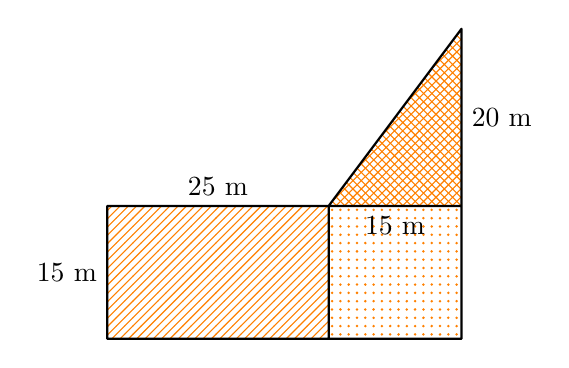
\begin{tikzpicture}[scale=0.9,line width=0.8pt,line join=round,>=stealth]
			\def\a{8}
			\fill[pattern=north east lines,pattern color=orange] (0,0) rectangle (-25/\a,-15/\a);
			\fill[pattern=dots,pattern color=orange] (0,0) rectangle (15/\a,-15/\a);
			\fill[pattern=crosshatch,pattern color=orange] (0,0) -- (15/\a,0)--(15/\a,20/\a) --cycle;
			\draw (0,0)--++(180:25/\a)node[midway,above]{25 m}
			--++(-90:15/\a)node[midway,left]{15 m}
			--++(0:25/\a)--++(90:15/\a)--++(0:15/\a)node[midway,below]{15 m}
			--++(-90:15/\a)--++(180:15/\a)--++(0:15/\a)--++(90:15/\a)--++(90:20/\a)node[midway,right]{20 m}
			--cycle
			;
		\end{tikzpicture}
	}
	
	\begin{listEX}
		\item Em hãy tính diện tích phần đất trồng hoa mẫu đơn.
		\item Biết chi phí để trồng một mét vuông hoa mẫu đơn là $220\,000$ đồng / $1$ m$^{2}$, hoa cúc $90\,000$ đồng / $1$ m$^{2}$ và hoa hồng là $160\,000$ đồng /$ 1$ m$^{2}$. Tính số tiền bác An phải bỏ ra để trồng hoa?
	\end{listEX} 	
	\loigiai{a) Diện tích đất trồng hoa mẫu đơn là $25\cdot 15=375$ (m$^2$) \\
		
		b) Số tiền bác An bỏ ra để trồng hoa là \\
		$375\cdot 220\,000 + 15\cdot 15\cdot 90\,000+\frac{15\cdot 20}{2}\cdot 160\,000=126\,750\,000$ (đồng)}
		\end{bt}

%%Câu 7.
\begin{bt} Cho bảng số liệu ban đầu về điểm kiểm tra môn Toán của học sinh lớp 6A như sau:
	\begin{center}
		\begin{tabular}{|c|c|c|c|c|c|c|c|c|c|}
			\hline
			6 & 9 & 9 & 7 & 10 & 9 & 10 & 10 & 7 & 8 \\
			\hline
			9 & 10 & 9 & 10 & 6 & 7 & 10 & 9 & 10 & 10 \\
			\hline
			6 & 7 & 8 & 9 & 10 & 6 & 10 & 9 & 10 & 10\\
			\hline
		\end{tabular}
	\end{center}
	\begin{listEX}
		\item Em hãy lập bảng thống kê theo mẫu sau: (học sinh vẽ bảng này vào bài làm)
		\begin{center}
			\begin{tabular}{|l|l|l|l|l|l|}
				\hline
				Điểm số & 6 & 7 & 8 & 9 & 10 \\
				\hline
				Số học sinh đạt được &  &  &  &  &  \\
				\hline
			\end{tabular}
		\end{center}
		\item Lớp 6A có bao nhiêu học sinh? Cho biết số học sinh đạt điểm Giỏi (từ điểm 8 trở lên) có bao nhiêu học sinh?
	\end{listEX} 
	
	
	\loigiai{
		a) \begin{center}
			\begin{tabular}{|l|l|l|l|l|l|}
				\hline
				Điểm số & 6 & 7 & 8 & 9 & 10 \\
				\hline
				Số học sinh đạt được & 4 & 4 & 2 & 8 & 12 \\
				\hline
			\end{tabular}
		\end{center}
		b) Lớp 6A có 30 học sinh, số học sinh đạt điểm giỏi có $2+8+12=22$ học sinh}
		\end{bt}
  
\Closesolutionfile{ansbook} 
\newpage
		
%%%%%%%%%%%%%% ĐỀ SỐ 3
\Opensolutionfile{ansbook}[ans/ansD3] 
%DS0



\section{ĐỀ SỐ \thesection }
\setcounter{bt}{0}
%%Câu 1.
\begin{bt} Thực hiện phép tính
	\begin{listEX}[2]
		\item $(-39)\cdot75+(-39)\cdot25$;
		\item $24:(-6)+6^2$;
		\item $[(-60):5+2\cdot(-8)]:(-2)^2+(-1)^{1024}$;
		\item $680-170:[(47-44)^2+(-2)^3\cdot2023^0]$.
	\end{listEX}
	\loigiai{
		\begin{listEX}[2]
				\item $(-39)\cdot75+(-39)\cdot25\\=(-39)\cdot(75+25)\\=(-39)\cdot100=-3900$
				\item $24:(-6)+6^2\\=-4+36\\=32$
				\item $\left[ (-60):5+2\cdot(-8)\right] :(-2)^2+(-1)^{1024}\\=(-12-16):4+1\\=-28:4+1\\=-7+1=-6$
				\item $680-170:\left[ (47-44)^2+(-2)^3\cdot2023^0\right] \\=680-170:(3^2-8\cdot1)\\=680-170:(9-8)\\=680-170:1=510$
		\end{listEX}
	}
\end{bt}


%%Câu 2.
\begin{bt} Tìm số nguyên $x$, biết:
	\begin{listEX}[2]
		\item $12\cdot x=-60$;
		\item $12\, \vdots\,  x$;
		\item $25+2\cdot(x-8)=5$;
		\item $(3x-5)-(x-2)=17$.
	\end{listEX}
	\loigiai{
		\begin{listEX}[2]
			\item $12\cdot x  = -60$\\
				\hspace*{0.72 cm}$\begin{aligned}
				x &= -60 : 12\\
				x &= -5
				\end{aligned}$
			\item 
				$12\,\vdots\,x \Rightarrow x \in \text{Ư}(12)$\\
				$x \in \{\pm1;\pm2;\pm3;\pm4;\pm6;\pm12\}$
			\item 	$25 + 2\cdot(x - 8) = 5$\\
				\hspace*{0.9 cm}$\begin{aligned}
				2\cdot(x - 8) &= -20\\
				x - 8 &= -10\\
				x &= -2
				\end{aligned}$
			\item $(3x - 5) - (x - 2)  = 17$\\
				\hspace*{2.1 cm}$\begin{aligned}
				3x - x &= 17 + 5 - 2\\
				2x &= 20\\
				x &= 10
				\end{aligned}$
		\end{listEX}
		
	}
\end{bt}



%%Câu 3.
\begin{bt} Một tòa nhà có 10 tầng (bao gồm tầng G) và 3 tầng hầm, tầng G được đánh số là tầng 0, hãy dùng phép cộng các số nguyên để diễn tả tình huống sau: Bạn Nam đang ở tầng 1, bạn sử dụng thang máy đi lên 5 tầng và sau đó đi xuống 8 tầng để lấy tài liệu. Hỏi cuối cùng, bạn Nam dừng thang máy ở tầng mấy?
	\loigiai{$1+5-8=-2$. Vậy bạn Nam đang ở tầng hầm số 2.}
\end{bt}


%%Câu 4.
\begin{bt} Một đội văn nghệ gồm 24 nam và 30 nữ được thầy giáo chia đều thành các nhóm để tập các tiết mục văn nghệ chào mừng Xuân Giáp Thìn. Hỏi:
	\begin{enumerate}
		\item Thầy giáo có thể chia nhiều nhất bao nhiêu nhóm văn nghệ?
		\item Mỗi nhóm có bao nhiêu nam, bao nhiêu nữ?
	\end{enumerate}
	\loigiai{
		\begin{enumerate}
			\item  Gọi $x$ $(x\in  \mathbb{N})$ là số nhóm nhiều nhất có thể chia. Ta có $x=\text{ƯCLN}(24,30)$\\
			Phân tích mỗi số ra thừa số nguyên tố 
				$24=2^3\cdot3$; \qquad $30=2\cdot3\cdot5$
				
			$x=\text{ƯCLN}(24,30)=2\cdot3=6$.
			
			Vậy có thể chia được nhiều nhất 6 nhóm.
			\item Mỗi nhóm có $24:6=4$ nam và $30:6=5$ nữ. 
		\end{enumerate}
	}
\end{bt}
%%Câu 5.
\begin{bt} Trường THCS S phát động chương trình quyên góp sách cũ để gửi cho trẻ em vùng sâu vùng xa. Số sách thu được đóng thành bó 40 quyển hay 50 quyển đều vừa đủ. Em hãy tính số sách quyên góp được, biết số sách quyên góp được khoảng từ 500 đến 700 quyển.
	\loigiai{Gọi $x$ $(x\in  \mathbb{N})$ là số quyển sách quyên góp được.
	Ta có $x\in \text{BC}(40,50)$ và $500<x<700$ \\
			Phân tích mỗi số ra thừa số nguyên tố 
		$40=2^3\cdot5$; \qquad $50=2\cdot5^2$.
		
		$\text{BCNN}(40,50)=2^3\cdot5^2=200 \\ \text{BC}(40,50)=B(200)=\{0;200;400;600;800;1000;...\}$.\\
		Mà $500<x<700$ nên $x=600$.\\
		Vậy có 600 quyển sách được quyên góp.}
\end{bt}

%%Câu 6.
\begin{bt} \immini[thm]{Ông Hải có một mảnh đất hình chữ nhật $ABCD$. Biết chiều rộng mảnh đất bằng 10 m và chiều dài mảnh đất bằng 20 m.
	}{
		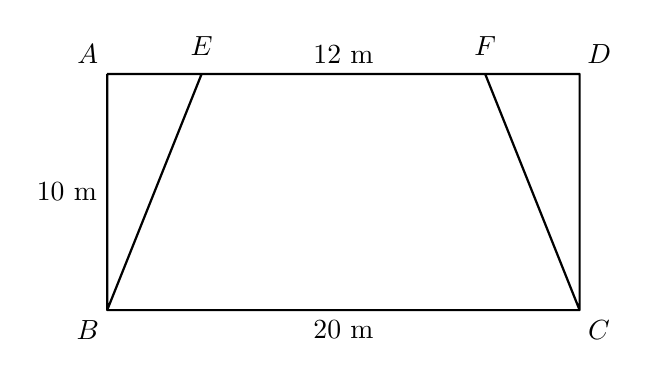
\begin{tikzpicture}[scale=1,line width=0.8pt,line join=round,>=stealth]
			\def\a{6} \def\b{3}  \def\c{1.2} 
			\path (0,0) coordinate (B)
			(0,\b) coordinate (A)
			(\a,\b) coordinate (D)
			(\a,0) coordinate (C)
			(\c,\b) coordinate (E)
			(\a-\c,\b) coordinate (F)
			;
			\draw (A)--(B)--(C)--(D)--(A)
			(E)--(B) (F)--(C)
			(B)--(A)node[midway,left]{10 m}
			(E)--(F)node[midway,above]{12 m}
			(B)--(C)node[midway,below]{20 m}
			;
			\foreach \x/ \goc in {A/135,B/-135,C/-45,D/45,E/90,F/90}  \fill (\x) circle (0pt)        
			($(\x)+(\goc:3.5mm)$) node {$\x$};
		\end{tikzpicture}
	}
	
	\begin{enumerate}
		\item Tính diện tích mảnh đất hình chữ nhật $ABCD$.
		\item Ông Hải dành phần đất ở giữa có dạng hình thang $BEFC$ để xây nhà xưởng. Biết đáy bé hình thang là $EF=12$ m. Em hãy giúp ông Hải tính diện tích phần đất xây nhà xưởng.
		\item Phần đất còn lại ông Hải dùng để trồng rau. Biết rằng cứ mỗi mét vuông đất thu hoạch được 4 kg rau và giá bán rau là $5\,000$ đồng/kg. Tính số tiền ông Hải thu được khi bán rau.
	\end{enumerate}
	\loigiai{
		\begin{enumerate}
			\item Diện tích mảnh đất: $10\cdot20=200$ (m$^2$)
			\item Diện tích đất xây nhà xưởng: $(12+20)\cdot10:2=160$ (m$^2$)
			\item Số tiền ông Hải thu được: $(200-160)\cdot4\cdot5\,000=800\,0000$ (đồng) 
		\end{enumerate}
	}
\end{bt}


%%Câu 7.
\begin{bt} Cho tổng sau: $S=1+2+3+4+5+\ldots+2023+2024+2025$. Chứng tỏ rằng $S\, \, \vdots\, \, 3$.
	\loigiai{ $S=1+2+3+4+5+\ldots+2023+2024+2025\\=(2025+1)\cdot2025:2=2026\cdot 2025:2=2026:2\cdot 2025=1013\cdot 2025$.\\ Vì $2+0+2+5=9\, \vdots\, 3$ nên $2025\,  \, \vdots\, \,  3$. Suy ra $S\,  \, \vdots\, \,  3$.}
\end{bt}





  
\Closesolutionfile{ansbook} 
\newpage
		
%%%%%%%%%%%%%% ĐỀ SỐ 4
\Opensolutionfile{ansbook}[ans/ansD4] 
%DS0



\section{ĐỀ SỐ \thesection }
\setcounter{bt}{0}
%%Câu 1.
\begin{bt}Thực hiện phép tính:
	\begin{listEX}[3]
		\item $(-33) + 45 + (-67)$;
		\item $28\cdot 69 + 28\cdot 31 + (-100)$;
		\item $75:\left[ (153 - 6\cdot 5^2)\cdot 8 + 2011^0\right] $.
	\end{listEX}
	\loigiai{
		\begin{listEX}[3]
			\item $(-33) + 45 + (-67)$\\
				$= 45 - 33 - 67$\\
				$= 12 - 67$\\
				$= -55$ 
			\item $28\cdot 69 + 28\cdot 31 + (-100)$\\
				$= 28(69 + 31) - 100$\\
				$= 28\cdot 100 - 100$\\
				$= 2800 - 100$
				$= 2700$ 
			\item $75:\left[ (153 - 6\cdot 5^2)\cdot 8 + 2011^0\right]$\\
				$= 75:\left[(153 - 150)\cdot 8 + 1\right]$\\
				$= 75:(3\cdot 8 + 1)$\\
				$= 75:25$
				$= 3$ 
		\end{listEX}
	}
\end{bt}


%%Câu 2.
\begin{bt} Tìm số nguyên $x$, biết
	\begin{listEX}[3]
		\item $6x + 15 = 75$;
		\item $x - 12 = -27$;
		\item $23 + (x - 5):4 = 3^8 :3^5$.
	\end{listEX}
	\loigiai{
		\begin{listEX}[3]
			\item $6x + 15  = 75$\\
				\hspace{2 cm}$\begin{aligned} 
				6x &= 75 - 15\\
				6x &= 60\\
				x &= 10
				\end{aligned}$ 
			\item 	$x - 12  = -27$\\
				\hspace{2 cm}$\begin{aligned} 
				x &= -27 + 12\\
				x &= -15
				\end{aligned}$ 
			\item $23 + (x - 5):4  = 3^8 : 3^5$\\
				\hspace{1 cm}$\begin{aligned} 
				23 + (x - 5):4 &= 3^3\\
				23 + (x - 5):4 &= 27\\
				(x - 5):4 &= 4\\
				x - 5 &= 16\\
				x &= 21
			\end{aligned}$
		\end{listEX}
		
	}
\end{bt}

%%Câu 3.
\begin{bt}
	Học sinh khối $6$ có $180$ bạn nữ và $102$ bạn nam tham gia văn nghệ. Cô phụ trách muốn chia ra thành các nhóm sao cho số nam và nữ mỗi nhóm đều bằng nhau. Hỏi có thể chia nhiều nhất bao nhiêu nhóm? Mỗi nhóm có bao nhiêu nam, bao nhiêu nữ?
	\loigiai{
		Gọi $x$ là số nhóm nhiều nhất có thể chia $(x\in \mathbb N)$\\
		$x =$ ƯCLN$(180;102)$
		
		$180=2^2\cdot 3^2\cdot 5\qquad  102=2\cdot 3\cdot 17$
		
		ƯCLN$(180;102)=2\cdot 3=6$\\
		Vậy có thể chia nhiều nhất 6 nhóm.
		Mỗi nhóm có $30$ bạn nữ và $17$ bạn nam.
	}
\end{bt}


%%Câu 4.
\begin{bt}
	\immini[thm]{Bác Hai có một mảnh vườn hình chữ nhật với chiều dài $30$ m và chiều rộng là $12$ m. Giữa mảnh vườn, bác đào một cái ao hình vuông để nuôi cá có độ dài cạnh $9$ m, phần còn lại của mảnh vườn bác dùng để trồng rau.
		\begin{enumerate}
			\item Tính diện tích trồng rau.
			\item Bác Hai đi mua hạt giống để trồng rau, biết cần gieo $20$ gram hạt giống trên 1 m$^2$ đất. Hỏi cần bao nhiêu gram hạt giống đề gieo hết phần đất trồng rau?
		\end{enumerate}
	}
	{
		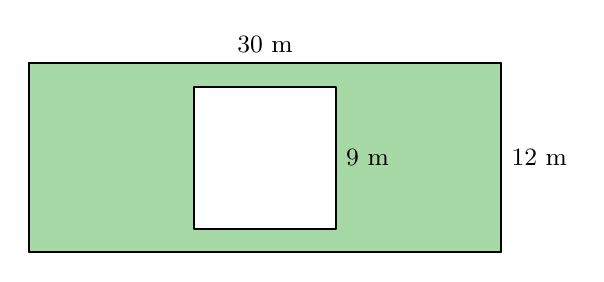
\begin{tikzpicture}[scale=1,line width=0.8pt,line join=round,>=stealth,font=\small]
			\def\s{5}
			;
			\draw[fill=white] (0,0) rectangle (30/\s,12/\s);
			\draw[fill=green!40!gray!50] (0,0) rectangle (30/\s,12/\s);
			\draw[fill=white] (10.5/\s,1.5/\s) rectangle (19.5/\s,10.5/\s); 
			\draw
			(19.5/\s,6/\s) node[right]{9 m}
			(30/\s,6/\s) node[right]{12 m}
			(15/\s,12/\s) node[above]{30 m}
			;
		\end{tikzpicture}
	}
	\loigiai{
		\begin{enumerate}
			\item Diện tích trồng rau là: $30\cdot12 - 9\cdot9 = 279$ (m$^2$).
			\item Số gram hạt giống cần để gieo hết phần đất trồng rau là: $20\cdot279 = 5\,580$ (g).
		\end{enumerate}
	}
\end{bt}


%%Câu 5.
\begin{bt}Một nhà sách nhập về một lô hàng gồm $40$ cái máy tính Casio-FX$570$ với giá $14\,000\,000$ đồng và bán ra với giá $400\,000$ đồng một máy. Sau khi bán được $20$ cái máy tính thì nhà sách giảm giá còn $380\,000$ đồng/máy và bán hết số máy tính còn lại. Hỏi nhà sách lời hay lỗ bao nhiêu tiền khi bán hết lô hàng trên?
	
	\loigiai{
		Số tiền thu được khi bán 20 cái máy tính đầu tiên là: 
			$20 \cdot 400\,000 = 8\,000\,000$ (đồng)
			
		Số tiền thu được khi bán hết số máy tính còn lại là: 
			$20 \cdot 380\,000 = 7\,600\,000$ (đồng)
			
		Số tiền nhà sách thu được khi bán hết 40 cái máy tính là: 
			$8\,000\,000 + 7\,600\,000 = 15\,600\,000$ (đồng)
			
		Vì $15\,600\,000$ đồng $> 14\,000\,000$ đồng nên nhà sách lời.
		 
		Số tiền nhà sách lời là: $15\,600\,000 - 14\,000\,000 = 1\,600\,000$ (đồng)
	}
\end{bt}


%%Câu 6.
\begin{bt} Tìm số nguyên tố $n$ sao cho $(3n+7)$ là bội của $(n+1)$.  
	
	\loigiai{Để $(3n+7)$ là bội của $(n+1)$ thì $(3n+7)$ phải chia hết cho $(n+1)$.\\
		Ta có: $3n+7 = 3(n+1) + 4$
		
		Để $3n+7$ chia hết cho $n+1$ thì $4$ phải chia hết cho $n+1$.
		
		Điều này có nghĩa là $(n+1)$ là ước của $4$.
		
		$(n+1)\in$Ư$(4)=\{\pm1, \pm2, \pm4\}$.
	$	\Rightarrow  n\in \{-5;-3;-2;0;1;3\}$\\
		Nên số nguyên tố $n$ thỏa mãn đề bài là $n = 3$.}
	
\end{bt}




 
\Closesolutionfile{ansbook} 
\newpage
	
%%%%%%%%%%%%%% ĐỀ SỐ 5
\Opensolutionfile{ansbook}[ans/ansD5] 
%DS0



\section{ĐỀ SỐ \thesection }
\setcounter{bt}{0}
%%Câu 1.
\begin{bt}  Thực hiện phép tính sau:
	
	\begin{listEX}[3]
		\item $-256 + 32 - 744$;
		\item $24\cdot15 + 24\cdot84 + 24$;
		\item $4\cdot5^2 - 3\cdot8 + 16:4 + 2017^0$.	
	\end{listEX}
	
	\loigiai{
		\begin{listEX}[3]
			\item $-256 + 32 - 744 \\= (-256 -744) + 32 \\= -1000 + 32  = -968$;
			\item $24\cdot15 + 24\cdot84 + 24\\ = 24 \cdot(15 + 84 + 1) \\= 2400$;
			\item  $4\cdot5^2 - 3\cdot8 + 16:4 + 2017^0 \\= 4\cdot25 - 24 + 4 + 1 \\= 81$.
		\end{listEX}
	}
\end{bt}


%%Câu 2.
\begin{bt} Tìm số nguyên $x$, biết
	\begin{listEX}[3]
		\item $4\cdot(x + 2) = 24$;
		\item $-x + 20 = 8$;
		\item $x \, \vdots \,  5$ và $9 < x < 30$.
	\end{listEX}
	
	\loigiai{
	\begin{listEX}[3]
			\item $4\cdot(x + 2)  = 24$\\
				\hspace*{0.85 cm}$\begin{aligned} 
				x + 2 &= 6\\
				x &= 4
				\end{aligned}$ 
			\item $-x + 20  = 8$\\
				\hspace*{1.25 cm}$\begin{aligned}
				x &= 20-8\\
				x &= 12
				\end{aligned}$
			\item 
				$x\,\vdots\,5 \Rightarrow x \in B(5)$\\
				$x \in \{10;15;20;25\}$
			\end{listEX}
	}
\end{bt}



%%Câu 3.
\begin{bt} Mai đi nhà sách mua dụng cụ học tập. Mai mua $5$ cuốn tập, $8$ cây viết bi, $2$ hộp bút màu. Biết giá một cuốn tập là $14\,000$ đồng, giá một hộp màu là $35\,000$ đồng, giá một cây viết bi là $7\,000$ đồng. Mai đưa cho quầy thu ngân $200\,000$  đồng. Hỏi Mai được trả lại bao nhiêu tiền?
	
	\loigiai{
		Tổng số tiền Mai đã mua hết là: $5\cdot14\,000 + 8\cdot7\,000 + 2\cdot 35\,000 = 196\,000$ (đồng) 
		\\Số tiền Mai được trả lại là: $200\,000 - 196\,000 = 4000$ (đồng)
	}
\end{bt}


%%Câu 4.
\begin{bt}
	Một trường tổ chức cho học sinh đi tham quan bằng ô tô, biết rằng nếu xếp $40$ người hay $45$ người vào một xe thì đều không dư. Tính số học sinh đi tham quan, biết số học sinh khoảng từ $600$ đến $800$.
	\loigiai{
		Gọi $x$ $(x\in  \mathbb{N})$ là số học sinh đi tham quan. Ta có $x \in BC(40;45)$ và $600 \leqslant x \leqslant 800)$\\
	Phân tích các số ra thừa số nguyên tố  $40=2^3\cdot5 \hspace{1cm}45=3^3\cdot5$
		\\ BCNN$(40;45) =2^3\cdot3^3\cdot5= 360$
		\\BC$(40;45) =$ B$(360)=\{0; 360;720;1080;... \}$
		\\Mà $x \in N, 600 \leqslant x < 800$
		\\Nên $x = 720$\\
		Vậy có 720 học sinh đi tham quan. 
	}
\end{bt}


%%Câu 5.
\begin{bt}Nhà bạn Hà có một mảnh vườn hình chữ nhật với chiều dài là $25$ m và chiều rộng là $18$ m. Bố bạn Hà muốn đào một cái ao hình vuông với cạnh là $6$ m ở giữa mảnh vườn để nuôi cá, phần còn lại để mẹ bạn trồng rau.
	\begin{enumerate}
		\item  Tính diện tích ao nuôi cá nhà Hà?
		\item Mẹ bạn Hà đi mua hạt giống để trồng rau, biết rằng cứ $1$ mét vuông đất gieo được $3$ gam hạt giống. Hỏi cần ít nhất bao nhiêu gam hạt giống để gieo hết phần đất trồng rau? 
	\end{enumerate}
	
	\loigiai{
		\begin{enumerate}
			\item Diện tích ao nuôi cá nhà bạn Hà: $6\cdot6 = 36$ (m$^2$)
			\item Diện tích mảnh vườn nhà bạn Hà là: $25\cdot18 = 450$ (m$^2$)
			\\ Diện tích phần đất trồng rau là: $450 - 36 = 414$ (m$^2$)
			\\ Lượng hạt giống cần để gieo hết phần đất trồng rau là: $414\cdot3 = 1242$ (gam)
		\end{enumerate}
	}
\end{bt}


%%Câu 6.
\begin{bt}Quan sát biểu đồ tranh dưới đây và trả lời câu hỏi: 
	\begin{center}
		\def\icon{\faApple* \ \ }
		\def\hicon{\tikz{\clip(-0.18,-0.19)rectangle(0.02,0.45);\path(0,0)node{\faApple*}}}
		\def\vetranh#1{\foreach \dem in{1,...,#1}{\icon \ }}{
			\begin{tabular}{|c|p{10cm}<{}|}\hline 
				\multicolumn{2}{|c|}{\bf Khối lượng táo một cửa hàng bán được của các ngày trong tuần}\\ \hline 
				\bf Ngày &\multicolumn{1}{c|}{\bf Số ki-lô-gam táo bán được}\\ \hline 
				Thứ 2 &\vetranh{6}\\ \hline 
				Thứ 3 &\vetranh{3} \hicon \\ \hline 
				Thứ 4 &\vetranh{5} \\ \hline 
				Thứ 5 &\vetranh{4} \hicon \\ \hline 
				Thứ 6 &\vetranh{4} \\ \hline 
				Thứ 7 &\vetranh{8}\\ \hline 
			\end{tabular}\\
			(Cho biết: \icon = 20 kg ;    \quad    \hicon \ \ = 10 kg)}
	\end{center}
	\begin{enumerate}
		\item Ngày nào cửa hàng bán được khối lượng táo nhiều nhất?
		\item Ngày nào cửa hàng bán được khối lượng táo ít nhất?
		\item Tính tổng khối lượng táo cửa hàng bán được trong tuần đó?
	\end{enumerate}
	
	\loigiai{
		\begin{enumerate}
			\item Ngày thứ 7 cửa hàng bán được khối lượng táo nhiều nhất.
			\item Ngày thứ 3 cửa hàng bán được khối lượng táo ít nhất.
			\item Khối lượng táo cửa hàng bán được trong tuần đó là: $30\cdot20 + 2\cdot10 = 620$ (kg)
		\end{enumerate}
	}
\end{bt}


%%Câu 7.
\begin{bt} Cho $A = 1 + 2 + 2^2 + 2^3 + 2^4 +...+ 2^{99} $. Chứng minh rằng $A$ không chia hết cho $7$. 
	\loigiai{
		$A = 1+2+2^2+2^3+2^4+...+2^{99}$
		\\$A = (1+2+2^2)+2^3(1+2+2^2)+...+2^{96}(1+2+2^2)+2^{97}$
		\\ $A = 7 + 2^3\cdot 7+...+2^{96}\cdot7+2^{97}$
		\\ $A = 7(1+2^3+...+2^{96})+2^{97}$ 
		\\Mà $7(1+2^3+...+2^{96})\vdots7$ và $2^{97}\not\vdots7$ 
	nên $A\, \not\vdots\, 7$
	}
\end{bt}




  
\Closesolutionfile{ansbook} 
\newpage
	
%%%%%%%%%%%%%% ĐỀ SỐ 6
\Opensolutionfile{ansbook}[ans/ansD6] 
\section{ĐỀ SỐ \thesection } %đề 18
\setcounter{bt}{0}

%%Câu 1.
\begin{bt} Cho tập hợp $D=\{x\in Z|-3<x\leq 1\}$. \\
	Em hãy viết lại tập hợp $D$ bằng cách liệt kê các phần tử.
	\loigiai{$D=\{-2;-1;0;1\}$}
\end{bt}


%%Câu 2.
\begin{bt} Tính nhanh (nếu có thể):
	\begin{listEX}[2]
		\item $66\cdot(-45)+(-55)\cdot66$;
		\item $257-7[(-3)^2-(17-16)^{2023}]$;
		\item $[(3^2+2^3)\cdot2-52:13]:(5\cdot3)$;
		\item $2[(25-3^{2024}:3^{2022}):2^2+149]-400$.
	\end{listEX}
	\loigiai{
		\begin{listEX}[2]
				\item $66\cdot(-45)+(-55)\cdot66\\
				=66(-45-55)\\
				=66\cdot(-100)
				=-6600$
				\item $257-7[(-3)^2-(17-16)^{2023}]\\=257-7[9-1]\\=257-7\cdot8=257-56=201$
				\item $[(3^2+2^3)\cdot2-52:13]:(5\cdot3)\\=[(9+8)\cdot2-4]:15\\=(17\cdot2-4)\cdot15\\=30:15\\=2$
				\item $2[(25-3^{2024}:3^{2022}):2^2+149]-400\\=2[(25-3^2):4+149]-400\\=2\cdot (16:4+149)-400\\=2\cdot153-400=-94$
			\end{listEX}
	}
\end{bt}



%%Câu 3.
\begin{bt} Tìm số nguyên $x$, biết:
	\begin{listEX}[2]
		\item $x-42=-8$;
		\item $(x+12):15=60$;
		\item $36+(100-5x):4=51$;
		\item $5(x+1)^2-21=-1$.
	\end{listEX}
	\loigiai{\begin{multicols}{2}
			\begin{enumerate}
				\item 
				$\begin{aligned}
					x - 42 &= -8\\
					x &= -8 + 42 = 34
				\end{aligned}$
				
				\item 
				$\begin{aligned}
					36 + (100 - 5x):4 &= 51\\
					(100 - 5x):4 &= 51 - 36 = 15\\
					100 - 5x &= 15\cdot4 = 60\\
					5x &= 100 - 60 = 40\\
					x &= 40:5 = 8
				\end{aligned}$
				
				\item 
				$\begin{aligned}
					(x + 12):15 &= 60\\
					x + 12 &= 60\cdot15 = 900\\
					x &= 900 - 12 = 888
				\end{aligned}$
				
				\item 
				$\begin{aligned}
					5(x + 1)^2 - 21 &= -1\\
					5(x + 1)^2 &= -1 + 21 = 20\\
					(x + 1)^2 &= 20:5 = 4
				\end{aligned}$\\
				$\Rightarrow x + 1 = 2$ hoặc $x + 1 = -2$\\
				$\Rightarrow x = 1$ hoặc $x = -3$
			\end{enumerate}
		\end{multicols}
		
	}
\end{bt}

%%Câu 4.
\begin{bt} An, Bình, Chi cùng học một đường. An cứ 5 ngày trực nhật một lần, Bình 10 ngày và Chi 8 ngày một lần. Lần đầu cả ba bạn cùng trực nhật vào một hôm. Hỏi sau ít nhất bao nhiêu ngày thì ba bạn lại cùng trực một hôm?
	\loigiai{Gọi $x$ $(x\in  \mathbb{N})$ là số ngày ít nhất để ba bạn lại cùng trực một hôm.Ta có $x=BCNN(5,10,8)$\\
		 Phân tích mõi số ra thừa số nguyên tố 
			$5=5$ \hspace{1cm} $10=2\cdot5$\hspace{1cm} $8=2^3$
		 
		$BCNN(5,10,8)=2^3\cdot5=40$.\\
		Vậy sau 40 ngày ba bạn lại cùng trực nhật một hôm.
	}
\end{bt}


%%Câu 5.

\begin{bt} \immini[thm]{
		Bác Bảo có một khu đất hình vuông có kích thước 35 m.
		\begin{enumerate}
			\item Tính chu vi và diện tích khu đất của bác Bảo.
			\item Bác Bảo chia mảnh đất làm hai như hình bên. Bác cần rào phần đất nuôi bò lại để làm chuồng. Hỏi bác Bảo cần bao nhiêu mét kẽm gai để vừa đủ rào mảnh đất làm chuồng bò? Tính diện tích chuồng bò.
		\end{enumerate}
	}{
		\begin{tikzpicture}[scale=1,line width=0.8pt,line join=round,>=stealth,font=\small]
			\def\s{9}
			;
			\draw[fill=white] (0,0) rectangle (35/\s,35/\s);
			\draw[fill=lightgray] (0,0) --(0,10/\s)--(35/\s,18/\s)node[midway,sloped,above]{36 m}--(35/\s,0)--cycle;
			\draw (0.5,30/\s) node[right]{Đất trồng cỏ} (35/\s-0.5,0.5)node[left]{Chuồng bò};
			\draw[<->] (-0.3,10/\s)--++(90:25/\s) node[midway,above, sloped]{25 m};
			\draw[<->] (35/\s+0.3,18/\s)--++(90:17/\s) node[midway,below,sloped]{17 m};
		\end{tikzpicture}
	}
	\loigiai{\begin{enumerate}
			\item Chu vi khu đất: $35\cdot4=140$ (m)\\Diện tích khu đất: $35\cdot35=1225$ (m$^2$)
			\item Số mét kẽm cần: $10+18+35+36=99$ (m) \\ Diện tích chuồng bò: $(35-25+35-17)\cdot35:2=490$ (m$^2$)
	\end{enumerate}}
\end{bt}



%%Câu 6.
\begin{bt} Vẽ Biểu đồ cột biểu diễn môn thể thao yêu thích của học sinh lớp 6A được cho trong bảng thống kê sau:
	\begin{center}
		\begin{tabular}{|c|c|c|c|c|}\hline
			\textbf{Môn thể thao}&\textbf{Bóng đá}&\textbf{Cầu lông}&\textbf{Bóng bàn}&\textbf{Bóng rổ} \\ \hline
			\textbf{Số học sinh yêu thích}&10&7&3&5 \\ \hline
		\end{tabular}\\
	\end{center}
	\loigiai{
		\begin{center}
			\begin{tikzpicture}
				[scale=0.8,font=\small,line join=round,>=stealth]
				\def\hoanh{10.2};
				\def\tung{4.2};
				\node[above] at (\hoanh/2,\tung+1){\normalsize \bfseries Môn thể thao yêu thích của học sinh lớp 6A};
				\def\mau{mauChuDao};
				\draw (0,0)node[left]{0}--(\hoanh,0);
				\draw[->] (0,0)--(0,\tung+1);
				\foreach \y in {2,4,...,12}{\draw (-0.1,\y/3)node[left]{$\y$}--++(0:0.2);
					\draw[dashed,gray] (0,\y/3)--(\hoanh-0.2,\y/3);}
				\foreach \x/\n in{2/10,4/7,6/3,8/5}{\draw[line width=7mm,\mau] (\x,0)--++(0,\n/3)node[black,shift={(90:0.3)}]{\n};}
				\foreach \x/\p in {2/Bóng đá,4/Cầu lông,6/Bóng bàn,8/Bóng rổ}{\node at (\x,-0.4){\footnotesize \p};} 
			\end{tikzpicture}
		\end{center}
	}
\end{bt}


%%Câu 7.
\begin{bt} Anh Long có tiền lương cố định hàng tháng là $8\,000\,000$ đồng. Nếu anh Long làm tăng ca thì được tính thêm $200\,000$ đồng một giờ và nếu anh làm sai kỹ thuật thì 1 lỗi sẽ bị trừ $150\,000$ đồng. Tháng 12, anh Long làm tăng ca 28 giờ và bị sai 4 lỗi kỹ thuật. Hỏi tiền lương thực lãnh của anh Long trong tháng 12 là bao nhiêu?
	
	\loigiai{Tiền lương của anh Long tháng 12 là:\\ $8\,000\,000+28\cdot200\,000-4\cdot150\,000=13\,000\,000$ (đồng)}
\end{bt}



 
\Closesolutionfile{ansbook} 
\newpage
		
%%%%%%%%%%%%%% ĐỀ SỐ 7
\Opensolutionfile{ansbook}[ans/ansD7] 
\section{ĐỀ SỐ \thesection }%ĐỀ 7
\setcounter{bt}{0}

%%Câu 1.
\begin{bt}\textbf{ }
	\begin{listEX}
		\item Liệt kê các số nguyên tố có 2 chữ số nhỏ hơn $20$.
		\item Sắp xếp các số nguyên sau theo thứ tự tăng dần: $34 ;\ -32 ;\ 43 ;\ -23$.
		\item Viết tập hợp $A$ gồm các ước tự nhiên của $27$.
	\end{listEX}
	\loigiai{a) $11; 13; 17; 19$ \hfill b) $-32;-23; 34; 43 $ \hfill c) $A = \{1, 3, 9, 27\}$}
\end{bt}



%%Câu 2.
\begin{bt} Thực hiện các phép tính:
	\begin{listEX}[2]
		\item $7^{25}: 7^{23}-2^{3} \cdot6+231^{0}$;
		\item $211:\left\{-200+\left[(-5 \cdot 14+65) \cdot 3+2^{2}\right]\right\}$.
	\end{listEX}
	\loigiai{a) 2 \hfill b) -1}
\end{bt}

%%Câu 3.
\begin{bt} \textbf{ }
	\begin{listEX}
		\item Tìm $x$, biết: $x+12=8 \cdot (-5)$.
		\item Tìm số nguyên $x$, biết: $128-3\cdot (x+4) = 23$.
		\item Một trường THCS tổ chức cho học sinh khối 6 đăng ký tham gia tiết học ngoài nhà trường tại bảo tàng Hồ Chí Minh. Trong ngày đi, nhà trường sắp xếp $30$ em hay $36$ em hay $40$ em lên một xe thì đều vừa đủ không thừa học sinh nào. Tính số học sinh khối 6 của trường đăng ký tham gia tiết học biết rằng số học sinh này khoảng $300$ đến $400$ học sinh.
	\end{listEX}
	\loigiai{a) -52 \hfill  b) 31 \hfill c) 360 học sinh}
\end{bt}


%%Câu 4.
\begin{bt} Một mảnh vườn hình chữ nhật có độ dài hai cạnh là $8$ m và $12$ m.
	\begin{listEX}
		\item Em hãy tính diện tích của mảnh vườn đó.
		\item Dọc theo các cạnh của mảnh vườn, người ta trồng các khóm hoa, cứ $2$ m trồng một khóm hoa. Tính số khóm hoa cần trồng.
	\end{listEX}
	\loigiai{a) 96 m$^2$ \hfill b) 20 khóm.}
\end{bt}

%%Câu 5.
\begin{bt} 
	\immini[thm]{
		Cho biểu đồ cột kép biểu diễn số học sinh giỏi của lớp 6A1. Từ biểu đồ bên, em hãy cho biết:
		\begin{listEX}
			\item Trong học kì 1, tổ nào có số học sinh giỏi nhiều nhất?
			\item Tính tổng số học sinh giỏi của cả lớp trong học kỳ 2?
		\end{listEX}
	}{
		\begin{tikzpicture}[scale=0.8,font=\small,line join=round,>=stealth]
			\def\hoanh{8} \def\tung{4} \def\sc{2.2}
			\node[above] at (\hoanh/2,\tung+1){\normalsize \bfseries Tình hình số học sinh giỏi của các tổ lớp 6A1};
			\def\mau{mauChuDao};
			\draw[->] (0,0)node[left]{0}--(\hoanh,0);
			\draw[->] (0,0)--(0,\tung+1);
			\foreach \y in {1,2,...,9}{\draw (-0.1,\y/\sc)node[left]{$\y$}--++(0:0.2);
				\draw[dashed,gray] (0,\y/\sc)--(\hoanh-0.2,\y/\sc);}
			\foreach \x/\n/\p in{1/3/5,3/2/4,5/6/6,7/1/8}{
				\draw[line width=5mm,\mau] (\x-0.3,0)--++(0,\n/\sc)node[black,shift={(90:0.2)},font=\footnotesize]{\n};
				\draw[line width=5mm,cyan] (\x+0.3,0)--++(0,\p/\sc)node[black,shift={(90:0.2)},font=\footnotesize]{\p};}
			\foreach \x/\p in {1/Tổ 1,3/Tổ 2,5/Tổ 3,7/Tổ 4}{\node at (\x,-0.4){\footnotesize \p};}        
			\fill[\mau] (1.5,\tung+0.8) rectangle (1.8,\tung +0.5) node [black,shift={(10:0.9)}]{Học kỳ 1};
			\fill[cyan] (4.5,\tung+0.8) rectangle (4.8,\tung +0.5) node [black,shift={(10:0.9)}]{Học kỳ 2};
		\end{tikzpicture}
	}
	\loigiai{a) Tổ 3 \hfill b) 23 học sinh}
\end{bt}



%%Câu 6.
\begin{bt} Bạn Lan đi nhà sách mua $12$ cây viết, $20$ quyển tập, $12$ cây thước. Biết $1$ cây viết có giá là $7\,000$ đồng, một quyển tập có giá là $12\,000$ đồng và giá một cây thước là $5\,000$ đồng. Hỏi:
	\begin{listEX}
		\item Bạn Lan đã mua hết tổng cộng bao nhiêu tiền?
		\item Với số tiền mang theo là $700\,000$ đồng thì bạn Lan có đủ để thanh toán số hàng trên hay không? Vì sao?
		\item Nhà sách đang có chương trình khuyến mãi: Mua $5$ cây viết tặng $1$ cây thước, mua $5$ quyển tập tặng $1$ cây viết, mua $10$ cây thước thì chỉ tính tiền $9$ cây. Khi áp dụng chương trình khuyến mãi ở trên, hỏi bạn Lan phải mua như thế nào để tổng số viết, tập, thước Lan mua và số viết, thước được tặng vẫn phải đủ $16$ cây viết, $20$ quyển tập, $12$ cây thước, giải thích cách mua và số tiền Lan phải trả khi áp dụng chương trình khuyến mãi là bao nhiêu?
	\end{listEX}
	\loigiai{a. 384 000 đồng \hfill b. Đủ tiền (vì $700>384)$ \hfill
		c. Mua 20 tập, 12 viết, 10  thước là $369\,000$.}
\end{bt}
 
\Closesolutionfile{ansbook} 
\newpage
	
%%%%%%%%%%%%%% ĐỀ SỐ 8
\Opensolutionfile{ansbook}[ans/ansD8] 
%DS0



\section{ĐỀ SỐ \thesection }
\setcounter{bt}{0}
%%Câu 1.
\begin{bt} Thực hiện phép tính:
	\begin{listEX}[3]
		\item $35-50+(-15)$; 
		\item $2^{3} \cdot 3^{2}-35: 5+2023^{0}$;
		\item $98+2 \cdot\left[\left(3^{2}+5\right): 7+1\right]$.
	\end{listEX}
	
\loigiai{a) $-30$ \hfill b) 66 \hfill c) 104}

\end{bt}


%%Câu 2. 
\begin{bt} Tìm $x$ biết:
	\begin{listEX}[3]
		\item $x+14=11+2x$;
		\item $3\cdot x-9=-36$;
		\item $(7-x) - (25+7 ) = -25$.
	\end{listEX}
	
	\loigiai{a) $3$ \hfill b) $-9$ \hfill c) 0}
	
	\end{bt}

%%Câu 3.
\begin{bt} Lớp 6A có $24$ học sinh nam và $20$ học sinh nữ. Trong buổi thi nghi thức đội, giáo viên chủ nhiệm lớp 6A đã yêu cầu lớp trưởng chia các bạn thành các nhóm sao cho giữa các nhóm phải có số học sinh nam bằng nhau, số học sinh nữ bằng nhau. Hỏi rằng lớp trưởng chia được nhiều nhất bao nhiêu nhóm?
	
	
\loigiai{$4$ nhóm}
\end{bt}


%%Câu 4.
\begin{bt} Bạn Yến được mẹ cho $500\,000$ đồng để đi nhà sách. Bạn đã mua $12$ quyển vở giá $10\,500$ đồng/quyển, $1$ bộ sách giáo khoa giá $190\,000$ đồng/bộ, $1$ bút chì giá $36\,000$ đồng/cây và $6$ bút gel với giá $8\,000$ đồng/cây.
	\begin{listEX}
		\item Hỏi bạn Yến đã mua hết bao nhiêu tiền?
		\item Với số tiền còn lại, bạn có thể mua được mấy ly kem Mixue biết giá 1 ly kem là $25\,000$ đồng/ly?
	\end{listEX}
	
\loigiai{a) $400\,000$ đồng \hfill b) $4$ ly kem}

	\end{bt}
	

%%Câu 5.
\begin{bt} Khu vườn hình chữ nhật có chiều rộng $12$ m và chiều dài gấp đôi chiều rộng. Tính diện tích của khu vườn.
	
\loigiai{288 m$^2$}
\end{bt}


%%Câu 6.
\begin{bt} Biểu đồ tranh dưới đây thể hiện số cây thông trang trí bán được trong 4 tuần của tháng 12 tại một cửa hàng.
	\begin{center}
		\def\icon{\faTree}
		\def\hicon{\tikz{\clip(-0.18,-0.17)rectangle(0,0.4);\path(0,0)node{\faTree}}}
		\def\vetranh#1{\foreach \dem in{1,...,#1}{\icon \ }}{
			\begin{tabular}{|c|p{6cm}<{}|}\hline 
				\multicolumn{2}{|c|}{\bf Số cây thông trang trí trong tháng 12}\\ \hline 
				\bf Tuần &\multicolumn{1}{c|}{\bf Số cây thông}\\ \hline 
				Tuần 1 &\vetranh{3}\hicon\\ \hline 
				Tuần 2 &\vetranh{5} \\ \hline 
				Tuần 3 &\vetranh{6}\hicon \\ \hline 
				Tuần 4 &\vetranh{8} \\ \hline 
			\end{tabular}\\
			(\icon = 10 xe cây thông;        \hicon = 5 cây thông)}
	\end{center}
		\begin{listEX}
			\item Lập bảng thống kê biểu diễn số cây thông trang trí bán được trong 4 tuần của tháng 12.
			\item Tính tổng số cây thông trang trí bán được trong 4 tuần của tháng 12.
		\end{listEX}
	
\loigiai{a) Học sinh tự lặp bảng \hfill b) 230 cây thông}

\end{bt}

%%Câu 7.
\begin{bt} Cho biểu thức: $A=7+7^{2}+7^{3}+7^{4}+7^{5}+\cdots+7^{2022}+7^{2023}$\\
Tìm $x$ để $6A+7=7^{x}$
\loigiai{$x=2024$}
\end{bt}
  
\Closesolutionfile{ansbook} 
\newpage
		
%%%%%%%%%%%%%% ĐỀ SỐ 9
\Opensolutionfile{ansbook}[ans/ansD9] 
%DS0



\section{ĐỀ SỐ \thesection }
\setcounter{bt}{0}
%%Câu 1.
\begin{bt} \textbf{}
	
	\begin{listEX}
		\item Thực hiện phép tính: $[53-(-12) \cdot 3 \cdot(-10)]$;
		\item Bỏ ngoặc rồi tính: $(177+222-185)-(67+22-75)$;
		\item Tìm số nguyên $x$ biết: $(x+5)(15x-30)=0$.
	\end{listEX}
	
\loigiai{a) $-307$ \hfill b) $200$ \hfill c) $x=-5, x=2$ 	}
\end{bt}


%%Câu 2.
\begin{bt} \textbf{ }
	\begin{listEX}
		\item  
		Tìm các số tự nhiên $x$ biết $42 \, \vdots \,  x$, $105 \, \vdots \, x$, $84 \, \vdots \, x$ và $x$ là bội của 3 . 
		\item 
		Số học sinh khối 6 của một trường trung học cơ sở trong khoảng từ $350$ đến $450$ em. Cô tổng phụ trách thấy rằng khi học sinh khối 6 xếp hàng $9$, hàng $10$, hàng $12$ đều thừa ra $3$ học sinh. Hỏi khối 6 của trường đó có bao nhiêu học sinh?
		
	\end{listEX}
	
	\loigiai{a) $x\in\{3;21 \}$ \hspace{2.5 cm} b) $363$ 	}
\end{bt}



%%Câu 3.
\begin{bt}
	Nhiệt độ trong một tủ cấp đông khi chưa bật là $23^{\circ} \mathrm{C}$. Khi bật tủ cấp đông, nhiệt độ bên trong tủ giảm $2^{\circ} \mathrm{C}$ mỗi phút. Hỏi phải mất bao nhiêu phút để nhiệt độ trong tủ đông đạt $-11^{\circ} \mathrm{C}$
	\loigiai{$17$ phút.}
\end{bt}


%%Câu 4.
\begin{bt}
	\immini[thm]{
		Trên một mảnh đất hình chữ nhật có chiều dài $12$ m, chiều rộng $10$ m người ta chia khu để trồng hoa, trồng cỏ: hoa sẽ được trồng ở khu vực hình bình hành $AMCN$, cỏ sẽ được trồng ở phần đất còn lại như hình vẽ. Tiền công để trả cho mỗi mét vuông trồng hoa là $50\,000$ đồng, trồng cỏ là $40\,000$ đồng.
		\begin{listEX}
			\item Tính diện tích mảnh đất hình chữ nhật, diện tích mảnh đất trồng hoa nêu trên.
			\item Tính số tiền công cần chi trả để trồng hoa và cỏ.
		\end{listEX}
	}{
		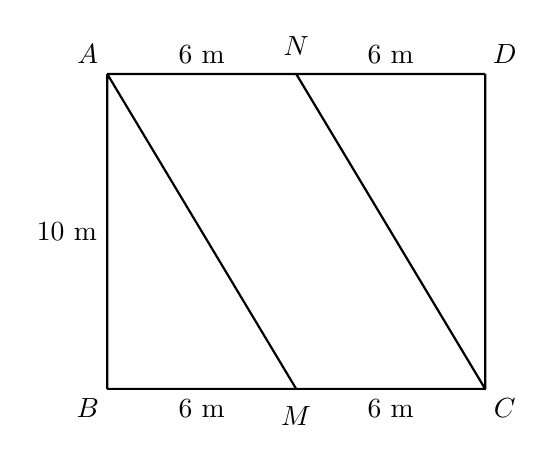
\begin{tikzpicture}[scale=1,line width=0.8pt,line join=round,>=stealth]
			\def\a{4.8} \def\b{4} 
			\path (0,0) coordinate (B)
			(0,\b) coordinate (A)
			(\a,\b) coordinate (D)
			(\a,0) coordinate (C)
			($(A)!0.5!(D)$) coordinate (N)
			($(B)!0.5!(C)$) coordinate (M)
			;
			\draw 
			(A)--(N)node[midway,above]{6 m}
			(D)--(N)node[midway,above]{6 m}
			(B)--(M)node[midway,below]{6 m}
			(M)--(C)node[midway,below]{6 m}
			(A)--(B)node[midway,left]{10 m}
			(A)--(M) (N)--(C)--(D)
			;
			\foreach \x/ \goc in {A/135,B/-135,C/-45,D/45,N/90,M/-90}  \fill (\x) circle (0pt)        
			($(\x)+(\goc:3.5mm)$) node {$\x$};
		\end{tikzpicture}
	}
	
	
	\loigiai{a) Diện tích mảnh đất là $120 $m$^2$, diện tích trồng hoa là $60 $m$^2$ \hspace{ 1 cm}
		b) $5\, 400\, 000$ }
\end{bt}


%%Câu 5.
\begin{bt}
	\immini[thm]{Cho biểu đồ cột kép biểu diễn số lượng học sinh yêu thích các môn thể thao của lớp 6A5
		\begin{listEX}
			\item Hãy cho biết môn thể thao nào có số lượng học sinh nữ và nam thích bằng nhau 
			\item Hãy cho biết các môn thể thao nào có số lượng học sinh nữ thích ít hơn số lượng học sinh nam và ít hơn bao nhiêu bạn.
		\end{listEX}
	}
	{\begin{tikzpicture}[scale=1,font=\small,line join=round,>=stealth]
			\def\hoanh{8} \def\tung{4} \def\sc{3.5}
			\def\mau{mauChuDao};
			\draw[->] (0,0)node[left]{0}--(\hoanh,0);
			\draw[->] (0,0)--(0,\tung+1);
			\foreach \y in {2,4,...,14}{\draw (-0.1,\y/\sc)node[left]{$\y$}--++(0:0.2);
				\draw[dashed,gray] (0,\y/\sc)--(\hoanh-0.2,\y/\sc);}
			\foreach \x/\n/\p in{1/6/13,3/10/10,5/12/10,7/14/5}{
				\draw[line width=5mm,\mau] (\x-0.3,0)--++(0,\n/\sc);
				\draw[line width=5mm,cyan] (\x+0.3,0)--++(0,\p/\sc);}
			\foreach \x/\p in {1/Bóng đá,3/Bóng bàn,5/Bóng rổ,7/Cầu lông}{\node at (\x,-0.4){\footnotesize \p};}        
			\fill[\mau] (1.5,\tung+0.8) rectangle (1.8,\tung +0.5) node [black,shift={(10:0.9)}]{Nữ};
			\fill[cyan] (4.5,\tung+0.8) rectangle (4.8,\tung +0.5) node [black,shift={(10:0.9)}]{Nam};
		\end{tikzpicture}
	}
	
	
	\loigiai{
	a) Bóng bàn \hfill b) Bóng đá (ít hơn $7$)
	 }
\end{bt}

%%Câu 6.
\begin{bt} So sánh
	$2^{777}$ và $7^{222}$.
	
	\loigiai{ $2^{777} > 7^{222}$. }
\end{bt}  
\Closesolutionfile{ansbook} 
\newpage
		
%%%%%%%%%%%%%% ĐỀ SỐ 10
\Opensolutionfile{ansbook}[ans/ansD10] 
%DS10_Trang
%Đề cũ số 10. Đề thường: chỉ đáp án; câu khó có hướng dẫn ngắn.

\section{ĐỀ SỐ \thesection }
\setcounter{bt}{0}

%% Dạng 1. Thực hiện phép tính — 4 ý: a cơ bản, b tính hợp lý, c và d nhiều ngoặc và lũy thừa.
\begin{bt} Thực hiện phép tính:
	\begin{listEX}
		\item $46+(-28)-13$;
		\item $(-15)\cdot 24+(-15)\cdot 16$;
		\item $96:\left[4^{2}-2^{3}\right]+(-1)^{2025}$;
		\item $(-3)^{2}\cdot 4-\left\{50-\left[2^{5}-7\cdot(-2)^{0}\right]\right\}$.
	\end{listEX}
	\loigiai{a) $5$ \hfill b) $-600$ \hfill c) $11$ \hfill d) $11$.}
\end{bt}

%% Dạng 2. Tìm x — 4 ý: a cơ bản, b trị tuyệt đối, c ngoặc lồng, d có x ở cả hai vế.
\begin{bt} Tìm số nguyên $x$, biết:
	\begin{listEX}
		\item $7x=-63$;
		\item $|4x-2|=18$;
		\item $3\left\{2\left[x-(-2)\right]-6\right\}=18$;
		\item $8-3(x-2)=2(x+1)-x$.
	\end{listEX}
	\loigiai{a) $x=-9$ \hfill b) $x=5$ hoặc $x=-4$ \hfill c) $x=4$ \hfill d) $x=3$.}
\end{bt}

%% Dạng 3. Tập hợp — 2 ý, số nguyên và số tự nhiên.
\begin{bt} Biết số $0$ là số tự nhiên. Gọi $A$ là tập hợp các số nguyên $x$ thỏa mãn $-9\le x\le 9$, $x$ chia hết cho $3$ và $x$ không chia hết cho $6$. Gọi $B$ là tập hợp các số tự nhiên nhỏ hơn $20$, chia hết cho $3$ và không chia hết cho $2$.
	\begin{enumerate}
		\item Liệt kê các phần tử của $A$ và của $B$.
		\item Liệt kê các số vừa thuộc $A$ vừa thuộc $B$. Liệt kê các số thuộc $A$ nhưng không thuộc $B$.
	\end{enumerate}
	\loigiai{a) $A=\{-9;\,-3;\,3;\,9\}$, $B=\{3;\,9;\,15\}$ \hfill b) Phần chung: $\{3;\,9\}$; thuộc $A$ nhưng không thuộc $B$: $\{-9;\,-3\}$.}
\end{bt}

%% Dạng 4. Ước và bội — thực tế cắt thanh gỗ, học sinh tự nhận ra ƯCLN.
\begin{bt} Người ta có những thanh gỗ dài $48$ cm và những thanh gỗ dài $36$ cm. Người ta cắt các thanh này thành những đoạn bằng nhau, dài nhất có thể, và không dư gỗ.
	\begin{enumerate}
		\item Mỗi đoạn dài bao nhiêu xăng-ti-mét?
		\item Mỗi thanh $48$ cm cắt được bao nhiêu đoạn? Mỗi thanh $36$ cm cắt được bao nhiêu đoạn?
	\end{enumerate}
	\loigiai{a) $12$ cm \hfill b) $4$ đoạn và $3$ đoạn.}
\end{bt}

%% Dạng 5. Toán thực tế — vận tốc, quãng đường, thời gian.
\begin{bt} Quãng đường từ nhà bạn Lan đến thư viện dài $2\,400$ m. Vận tốc đi bộ của bạn Lan là $80$ m/phút. Vận tốc đi xe đạp gấp $3$ lần vận tốc đi bộ.
	\begin{enumerate}
		\item Bạn Lan đi bộ hết bao nhiêu phút?
		\item Bạn Lan đi xe đạp hết bao nhiêu phút?
		\item Đi xe đạp ít hơn đi bộ bao nhiêu phút?
	\end{enumerate}
	\loigiai{a) $30$ phút \hfill b) $10$ phút \hfill c) $20$ phút.}
\end{bt}

%% Dạng 6. Hình học thực tế — lối đi bao quanh sân.
\begin{bt}
	\immini[thm]{
		Một mảnh vườn hình chữ nhật dài $25$ m, rộng $16$ m. Xung quanh vườn, sát bốn cạnh, có một lối đi rộng $2$ m. Phần bên trong lối đi dùng để trồng hoa.
		\begin{enumerate}
			\item Tính diện tích phần trồng hoa.
			\item Tính diện tích lối đi.
			\item Biết giá lát lối đi là $200\,000$ đồng/m$^{2}$. Tính số tiền lát lối đi.
		\end{enumerate}
	}{
		\begin{tikzpicture}[scale=0.22,line width=0.8pt,line join=round,>=stealth]
			\draw (0,0) rectangle (25,16);
			\draw (2,2) rectangle (23,14);
			\node at (12.5,8) {Trồng hoa};
			\draw[<->] (0,-1.4)--(25,-1.4) node[midway,below]{$25$ m};
			\draw[<->] (26.2,0)--(26.2,16) node[midway,right]{$16$ m};
			\draw[<->] (-1.2,14)--(-1.2,16) node[midway,left]{$2$ m};
		\end{tikzpicture}
	}
	\loigiai{a) $252$ m$^{2}$ \hfill b) $148$ m$^{2}$ \hfill c) $29\,600\,000$ đồng.}
\end{bt}

%% Dạng 7. Nâng cao — rút gọn thương của hai tổng lũy thừa cùng cơ số.
\begin{bt} Tính nhanh:
	\[
	\left(2^{7}+2^{8}+2^{9}\right):\left(2^{5}+2^{6}+2^{7}\right).
	\]
	\loigiai{Hướng dẫn: đặt thừa số chung $2^{7}$ ở tử và $2^{5}$ ở mẫu.\\
		Kết quả bằng $4$.}
\end{bt}
 
\Closesolutionfile{ansbook} 
\newpage
	
%%%%%%%%%%%%%% ĐỀ SỐ 11
\Opensolutionfile{ansbook}[ans/ansD11] 
\section{ĐỀ SỐ \thesection } %LÊ LỢI %Đề 11
\setcounter{bt}{0}

%%Câu 1.
\begin{bt} Tính hợp lý:
	\
	\begin{listEX}[2]	
		\item $131+(-74)+124+(-31)$;
		\item $(-2)^{2} \cdot 38-5 \cdot(-2)^{2}+67 \cdot(-2)^{2}$.
	\end{listEX} 
	\loigiai{a) $150$ \hfill b) $400$.}
\end{bt}


%%Câu 2.
\begin{bt} Tìm số nguyên $x$, biết
	\begin{listEX}[3]
		\item  $30-x=120$;
		\item $-3 \leq x \leq 2$;
		\item $(x-2) \cdot 8+12=(-84)$.
		\end{listEX}
	\loigiai{
	a) $x=-90$ \hfill b) $x\in \{-3;-2;-1;0;1;2\}$ \hfill c) $x=-10$.
	}
\end{bt}



%%Câu 3.
\begin{bt} Bác Dũng có một mảnh vườn hình chữ nhật với chiều dài 20 mét và chiều rộng là 12 mét. Giữa mảnh vườn bác đào một cái ao hình vuông có cạnh 8 mét để nuôi cá, phần còn lại của mảnh vườn bác dùng để trồng rau.
	\immini{
		\begin{enumerate}
			\item Tính chu vi mảnh vườn.
			\item Tính diện tích trồng rau.
			\item Bác Dũng đi mua hạt giống để trồng rau, biết cần gieo 3 gam hạt giống trong 1 mét vuông đất. Hỏi cần bao nhiêu gam hạt giống để gieo hết phần đất trồng rau?
	\end{enumerate}
	}
	{
	\begin{tikzpicture}[scale=1,line width=0.8pt,line join=round,>=stealth,font=\small]
		\def\s{3.2}
		;
		\draw[fill=white] (0,0) rectangle (20/\s,12/\s);
		\draw[pattern=north east lines,pattern color=lightgray] (0,0) rectangle (20/\s,12/\s);
		\draw[fill=white] (6/\s,2/\s) rectangle (14/\s,10/\s); 
		\draw
		(3/\s,6/\s) node{Trồng rau}
		(17/\s,6/\s) node{Trồng rau}
		(10/\s,6/\s) node{Ao cá}
		(10/\s,2/\s) node[below]{8 m}
		(20/\s,6/\s) node[right]{12 m}
		(10/\s,12/\s) node[above]{20 m}
		;
	\end{tikzpicture}
	}

	
	\loigiai{a) 64 m \hfill b) 176 m$^2$ \hfill c) $528$ gam.
	}
\end{bt}


%%Câu 4.
\begin{bt} Số liệu điểm kiểm tra môn Toán giữa học kỳ I của học sinh tổ 2 lớp 6A được ghi lại trong bảng dữ liệu như sau:
	
	\begin{center}
		\begin{tabular}{|c|c|c|c|c|c|}
			\hline
			8 & 10 & 9 & 9 & 7 & 7 \\
			\hline
			9 & 7 & 8 & 7 & 10 & 9 \\
			\hline
		\end{tabular}
	\end{center}
	\
	\begin{enumerate}
		\item  Em hãy cho biết bảng dữ liệu trên đang điều tra về vấn đề gì?
		\item Hãy lập bảng thống kê tương ứng và cho biết tổ 2 lớp 6 A có bao nhiêu thành viên.
	\end{enumerate}
	
	\loigiai{
		\begin{enumerate}
			\item Bảng dữ liệu trên đang điều tra về điểm kiểm tra môn Toán giữa học kỳ I của học sinh tổ 2 lớp 6A. Các số liệu trong bảng đại diện cho điểm số của từng học sinh trong kỳ kiểm tra này.
			\item 
		\begin{tabular}{|c|c|}
			\hline
			\text{Điểm} & \text{Số học sinh} \\
			\hline
			7 & 4 \\
			8 & 2 \\
			9 & 4 \\
			10 & 2 \\
			\hline
		\end{tabular}
	
		
		Tổ 2 lớp 6A có tổng cộng 12 thành viên.
		\end{enumerate}
	}
\end{bt}


%%Câu 5.
\begin{bt} 
Học sinh của một trường THCS khi xếp hàng $20,\,25,\ 30$ em đều thừa 15 em nhưng khi xếp thành hàng 41 em thì vừa đủ hàng. Hỏi trường đó có bao nhiêu học sinh, biết rằng, số học sinh trường đó chưa đến 1000 em.
	\loigiai{ 615 học sinh.
	}
	
\end{bt}


%%Câu 6.
\begin{bt}
Tính nhanh: $\left(4^{234}+4^{235}+4^{236}\right):\left(4^{232}+4^{233}+4^{234}\right)$.
	
	\loigiai{16.}
		




\end{bt}  
\Closesolutionfile{ansbook} 
\newpage
	
%%%%%%%%%%%%%% ĐỀ SỐ 12
\Opensolutionfile{ansbook}[ans/ansD12] 
%DS12_Trang
%Đề cũ số 12. Đề thường: chỉ đáp án; câu khó có hướng dẫn ngắn.

\section{ĐỀ SỐ \thesection }
\setcounter{bt}{0}

%% Dạng 1. Thực hiện phép tính — 4 ý: a cơ bản, b tính hợp lý, c và d nhiều ngoặc và lũy thừa.
\begin{bt} Thực hiện phép tính:
	\begin{listEX}
		\item $33+(-47)+9$;
		\item $(-12)\cdot 25+(-12)\cdot 15+(-12)\cdot 10$;
		\item $\left\{2^{5}-\left[18-(-3)^{2}\right]\right\}\cdot(-2)+4^{0}$;
		\item $200-8\cdot\left[5^{2}-3\cdot\left(2^{3}-6^{0}\right)\right]$.
	\end{listEX}
	\loigiai{a) $-5$ \hfill b) $-600$ \hfill c) $-45$ \hfill d) $168$.}
\end{bt}

%% Dạng 2. Tìm x — 4 ý: a cơ bản, b trị tuyệt đối, c nhiều ngoặc, d có x ở cả hai vế.
\begin{bt} Tìm số nguyên $x$, biết:
	\begin{listEX}
		\item $4x=-28$;
		\item $|3x-9|=6$;
		\item $2(3x-4)-5(x-2)=7$;
		\item $3(2x-1)-x=4(x-2)+5$.
	\end{listEX}
	\loigiai{a) $x=-7$ \hfill b) $x=5$ hoặc $x=1$ \hfill c) $x=5$ \hfill d) $x=0$.}
\end{bt}

%% Dạng 3. Tập hợp — 2 ý, số nguyên và số tự nhiên.
\begin{bt} Biết số $0$ là số tự nhiên. Gọi $H$ là tập hợp các số nguyên $x$ thỏa mãn $-8\le x<7$ và $|x|$ chia hết cho $3$. Gọi $K$ là tập hợp các số tự nhiên nhỏ hơn $12$, không chia hết cho $2$ và chia hết cho $3$.
	\begin{enumerate}
		\item Liệt kê các phần tử của $H$.
		\item Liệt kê các số vừa thuộc $H$ vừa thuộc $K$. Liệt kê các số thuộc $H$ nhưng không phải số tự nhiên.
	\end{enumerate}
	\loigiai{a) $H=\{-6;\,-3;\,0;\,3;\,6\}$ \hfill b) Phần chung: $\{3\}$; thuộc $H$ nhưng không phải số tự nhiên: $\{-6;\,-3\}$.}
\end{bt}

%% Dạng 4. Ước và bội — thực tế chia hoa, học sinh tự nhận ra ƯCLN.
\begin{bt} Cô Lan có $42$ bông hồng và $28$ bông cúc. Cô cắm hết số hoa vào các lọ sao cho các lọ có số hồng bằng nhau, số cúc bằng nhau, và mỗi lọ có cả hai loại hoa.
	\begin{enumerate}
		\item Nếu số lọ lớn hơn $1$, cách cắm nào khiến mỗi lọ có nhiều hoa nhất? Khi đó có bao nhiêu lọ, mỗi lọ có bao nhiêu bông hồng và bao nhiêu bông cúc?
		\item Nếu muốn có nhiều lọ nhất thì có bao nhiêu lọ? Mỗi lọ có bao nhiêu bông hồng và bao nhiêu bông cúc?
	\end{enumerate}
	\loigiai{a) $2$ lọ; mỗi lọ $21$ bông hồng và $14$ bông cúc \hfill b) $14$ lọ; mỗi lọ $3$ bông hồng và $2$ bông cúc.}
\end{bt}

%% Dạng 5. Toán thực tế — chia đều số lượng, một đáp án trong khoảng cho trước.
\begin{bt} Một kho phát khẩu trang. Chia đều cho $20$ người hoặc cho $30$ người thì đều hết số khẩu trang, không dư chiếc nào. Biết trong kho có nhiều hơn $250$ chiếc và ít hơn $320$ chiếc. Hỏi kho có bao nhiêu chiếc khẩu trang?
	\loigiai{$300$ chiếc.}
\end{bt}

%% Dạng 6. Hình học thực tế — mảnh đất hình chữ L.
\begin{bt}
	\immini[thm]{
		Từ một mảnh đất hình chữ nhật dài $20$ m, rộng $12$ m, người ta cắt đi một hình chữ nhật $8$ m $\times$ $5$ m ở một góc để làm lối ra. Phần còn lại dùng để trồng rau, như hình vẽ.
		\begin{enumerate}
			\item Tính diện tích đất trồng rau.
			\item Tính chu vi phần đất trồng rau.
			\item Cứ mỗi mét vuông thu hoạch được $5$ kg rau. Giá bán là $9\,000$ đồng/kg. Tính số tiền thu được khi bán hết số rau.
		\end{enumerate}
	}{
		\begin{tikzpicture}[scale=0.28,line width=0.8pt,line join=round,>=stealth]
			\draw (0,0)--(12,0)--(12,5)--(20,5)--(20,12)--(0,12)--cycle;
			\node at (8,8) {Trồng rau};
			\draw[<->] (0,-1.2)--(12,-1.2) node[midway,below]{$12$ m};
			\draw[<->] (12.7,0)--(12.7,5) node[midway,right]{$5$ m};
			\draw[<->] (12,4.2)--(20,4.2) node[midway,below]{$8$ m};
			\draw[<->] (20.8,5)--(20.8,12) node[midway,right]{$7$ m};
			\draw[<->] (0,12.8)--(20,12.8) node[midway,above]{$20$ m};
			\draw[<->] (-1.4,0)--(-1.4,12) node[midway,left]{$12$ m};
		\end{tikzpicture}
	}
	\loigiai{a) $200$ m$^{2}$ \hfill b) $64$ m \hfill c) $9\,000\,000$ đồng.}
\end{bt}

%% Dạng 7. Nâng cao — so sánh lũy thừa bằng cách đưa về cùng cơ số.
\begin{bt} So sánh $2^{20}$ và $8^{6}$.
	\loigiai{Hướng dẫn: viết $8^{6}=(2^{3})^{6}=2^{18}$.\\
		Vì $20>18$ nên $2^{20}>2^{18}$. Vậy $2^{20}>8^{6}$.}
\end{bt}
  
\Closesolutionfile{ansbook} 
\newpage
		
%%%%%%%%%%%%%% ĐỀ SỐ 13
\Opensolutionfile{ansbook}[ans/ansD13] 
\section{ĐỀ SỐ \thesection } %DỀ 13 QUẬN 6
\setcounter{bt}{0}

%%Câu 1.
\begin{bt} Thực hiện các phép tính
	\begin{listEX}[2]
		\item $345 + (-120) + (-275) + 400$;
		\item $3^{4} \cdot 3^{2} : 3^{5} - \left\{2 \cdot \left[50 - \left(12 - 2^{2} \cdot 3\right)\right]\right\}$.
	\end{listEX}
	\loigiai{a) $350$ \hfill b) $-97$.
	}
\end{bt}


%%Câu 2.
\begin{bt}Tìm  $x$ biết:
	\begin{listEX}[2]
		\item $25 + 4 \cdot x = 81$
		\item  $3^{2x} - 27 = 54$
	\end{listEX}
	\loigiai{a) $x=14$ \hfill b) $x=2$.
	}
\end{bt}



%%Câu 3.
\begin{bt}
	 	Hình dưới đây mô tả cửa xếp tự động. Mỗi khung như hình 3.1 được nối bởi các thanh inox có dạng hình thoi cạnh 30 cm.
	 \begin{center}
	 	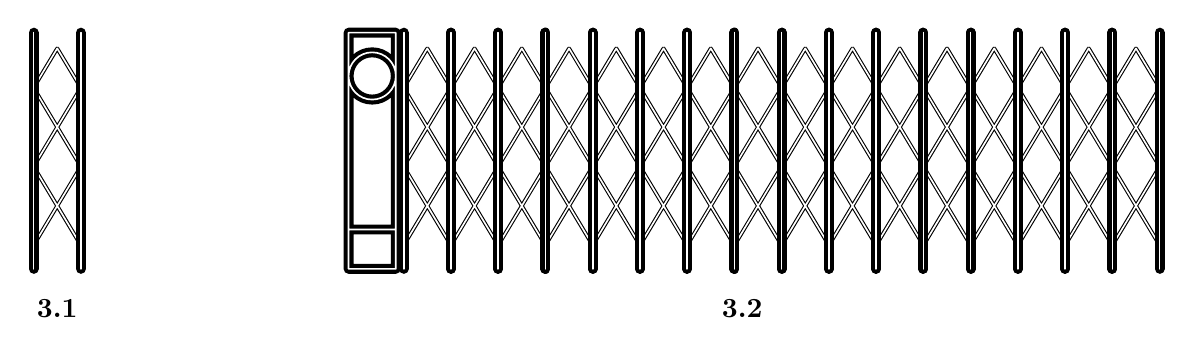
\begin{tikzpicture}[line cap=round,line join=round]
	 		% Define the basic properties
	 		\def\postheight{3}
	 		\def\postwidth{0.2}
	 		\def\crosslength{0.5}
	 		\def\gap{0.6}
	 		\def\sections{8}
	 		
	 		% Draw the closed gate (3.1)
	 		\begin{scope}[shift={(0,0)}]
	 			\draw[double] (0,0.3) -- (\gap,1.3) (0,1.3) -- (\gap, 2.3) (0,2.3) -- (\gap/2,2.8)
	 			(0,1.3) -- (\gap,0.3) (0,2.3) -- (\gap, 1.3) (\gap/2,2.8) -- (\gap,2.3);
	 			\draw[double,line width=1.5pt] (0,0) -- (0,\postheight) (\gap,0) -- (\gap,\postheight);
	 		\end{scope}
	 		
	 		% Draw the open gate (3.2)
	 		\begin{scope}[shift={(4,0)}]
	 			\draw[double,line width=1.5pt] (0,0) rectangle (\gap,\postheight)
	 			(0,0) rectangle (\gap,0.5) (0,\postheight-0.5) rectangle  (0,\postheight-0.5-\gap)
	 			(\gap/2,\postheight-0.25-\gap/2) circle (\gap/2);
	 			% Draw the open sections of the gate
	 			\foreach \i in {1,2,...,16} {
	 				\begin{scope}[shift={(\i*\gap+0.1,0)}]
	 					\draw[double] (0,0.3) -- (\gap,1.3) (0,1.3) -- (\gap, 2.3) (0,2.3) -- (\gap/2,2.8)
	 					(0,1.3) -- (\gap,0.3) (0,2.3) -- (\gap, 1.3) (\gap/2,2.8) -- (\gap,2.3);
	 					\draw[double,line width=1.5pt] (0,0) -- (0,\postheight) (\gap,0) -- (\gap,\postheight);
	 				\end{scope}
	 			}
	 		\end{scope}
	 		
	 		% Add labels below each part
	 		\node at (0.3,-0.5) {\textbf{3.1}};
	 		\node at (9,-0.5) {\textbf{3.2}};
	 	\end{tikzpicture}
	 \end{center}
	 \begin{enumerate}
	 \item  Hỏi mỗi khung như hình 3.1 cần bao nhiêu mét thanh inox để nối?
	 \item Hỏi cửa xếp tự động ở hình 3.2 cần bao nhiêu mét thanh inox để nối?
	 \end{enumerate}
	\loigiai{a) $3$ m \hfill b) $48$ m.
	}
\end{bt}


%%Câu 4.
\begin{bt} Một nhà máy sản xuất có ba loại sản phẩm: sản phẩm A, sản phẩm B và sản phẩm C. Số lượng mỗi loại sản phẩm là:
	\begin{multicols}{3}
		\begin{itemize}
			\item Sản phẩm A: 48 cái.
			\item Sản phẩm B: 72 cái.
			\item Sản phẩm C: 108 cái.
		\end{itemize}
	\end{multicols}
	
	Nhà máy muốn đóng gói tất cả sản phẩm vào các thùng sao cho mỗi thùng chứa số sản phẩm bằng nhau mà không để thừa sản phẩm. Hỏi mỗi thùng sẽ chứa bao nhiêu sản phẩm và nhà máy có thể đóng được tối đa bao nhiêu thùng?
	\loigiai{Mỗi thùng sẽ chứa: $19$ sản phẩm. Và nhà máy có thể đóng được tối đa $12$ thùng.}
\end{bt}



%%Câu 5.
\begin{bt} 
	Một gian phòng có nền hình chữ nhật với kích thước là $3,6 \mathrm{~m}$ và $5,8 \mathrm{~m}$, có một cửa sổ hình chữ nhật kích thước là $0,8 \mathrm{~m}$ và $1,2 \mathrm{~m}$ và một cửa ra vào hình chữ nhật kích thước $1,2 \mathrm{~m}$ và 2 m . Tỉ lệ phần trăm diện tích các cửa so với diện tích nền nhà.
	\loigiai{Tỉ lệ phần trăm diện tích các cửa và diện tích nền nhà là $\frac{3,36}{20,88} \approx 16 \%$.
	}
\end{bt}


%%Câu 6.
\begin{bt} 
	Biểu đồ cột kép ở hình vẽ biểu diễn số lượng ca nhiễm SAR-COVID-2 và số lượng người tử vong (tính đến ngày $3 / 7 / 2021$ tại Việt Nam). Hỏi tỉ lệ tử vong vì SAR-COVID-2 ở tỉnh nào là cao nhất? Cho các tỉ lệ đó là bao nhiêu.
	\begin{center}
	\begin{tikzpicture}[scale=0.07,font=\small,line join=round,>=stealth]
		% --- Thông số ---
		\def\hoanh{100} 
		\def\tung{150}   % chiều cao trục tung đủ lớn để chứa cột 174
		\def\sc{5}       % hệ số tỉ lệ, chia giá trị thực để vừa trang
		\def\w{5}        % bề rộng mỗi cột
		
		% --- Trục toạ độ ---
		\draw[->] (0,0)node[left]{0}--(\hoanh,0) node[right,below]{\footnotesize \textbf{Tỉnh}};
		\draw[->] (0,0)--(0,\tung/\sc+10) node[above]{\footnotesize \textbf{Số lượng (Người)}};
		
		% --- Chia vạch tung ---
		\foreach \y in {50,100,...,200}{
			\draw (-0.15,\y/\sc) node[left]{$\y$} -- ++(0:0.3);
		}
		
		% --- Cột dữ liệu ---
		\foreach \x/\nhiem/\chet in {10/126/10,30/113/7,50/56/12,70/174/23}{
			% Nhiễm (kẻ xéo)
			\fill[pattern=north east lines,pattern color=blue!80!black,draw=blue!80!black]
			(\x-\w,0) rectangle ++(\w,\nhiem/\sc);
			\node[black,font=\footnotesize,anchor=south,yshift=1pt]
			at (\x-\w/2,\nhiem/\sc) {\nhiem};
			
			% Chết (chấm bi)
			\fill[pattern=dots,pattern color=red!80!black,draw=red!70!black]
			(\x,0) rectangle ++(\w,\chet/\sc);
			\node[black,font=\footnotesize,anchor=south,yshift=1pt]
			at (\x+\w/2,\chet/\sc) {\chet};
		}
		
		% --- Nhãn tên các tỉnh ---
		\foreach \x/\p in {15/Hưng~Yên,35/Nghệ~An,55/Đồng~Tháp,75/Phú~Yên}{
			\node[font=\footnotesize,rotate=15,anchor=north east] at (\x,-0.5){\textbf{\p}};
		}
		
		\fill[pattern=north east lines,pattern color=blue!80!black,draw=blue!80!black]
		(84,38) rectangle (87,35);
		\node[font=\footnotesize,anchor=west] at (87.2,35) {Nhiễm};
		
		\fill[pattern=dots,pattern color=red!80!black,draw=red!70!black]
		(84,42) rectangle (87,39);
		\node[font=\footnotesize,anchor=west] at (87.2,40.5) {Chết};
		
	\end{tikzpicture}	\vspace{0.1 em}
	{\footnotesize\itshape (Nguồn: https://vnexpress.net/)}
	\end{center}
	
	

	
	
	
	\loigiai{
			Tỉ lệ tử vong vì SAR-COVID-2 ở tỉnh Hưng Yên là $\frac{10}{126} \approx 7,94 \%$.\\
			 Tỉ lệ tử vong vì SAR-COVID-2 ở tỉnh Nghệ An là $\frac{7}{113} \approx 6,19 \%$.\\
			Tỉ lệ tử vong vì SAR-COVID-2 ở tỉnh Đồng Tháp là $\frac{12}{56} \approx 21,43 \%$.\\
			Tỉ lệ tử vong vì SAR-COVID-2 ở tỉnh Phú Yên là $\frac{23}{174} \approx 13,22 \%$.\\
			Vậy tỉ lệ tử vong vì SAR-COVID-2 ở tỉnh Đồng Tháp là cao nhất
	}
\end{bt}


  
\Closesolutionfile{ansbook} 
\newpage
		
%%%%%%%%%%%%%% ĐỀ SỐ 14
\Opensolutionfile{ansbook}[ans/ansD14] 
\section{ĐỀ SỐ \thesection } % ĐỀ 14 Lê quý đôn q3
\setcounter{bt}{0}

%%Câu 1.
\begin{bt} \
	\begin{enumerate}
		\item Điền chữ số vào dấu * để được số $\overline{4 *}$ là số nguyên tố.
		\item Cho tập hợp $A=\{x \in \mathbb{Z} \mid-4<x<1\}$. Hãy viết tập hợp $A$ bằng cách liệt kê các phần tử.
		\item Hoàn thành bảng dưới đây vào giấy làm bài:
		
		\begin{center}
			\begin{tabular}{|l|c|c|}
				\hline
				Số La Mã & XIV & XIX \\
				\hline
				Giá trị tương ứng trong hệ thập phân & 14 &  \\
				\hline
			\end{tabular}
		\end{center}
		
	\end{enumerate}
	
	\loigiai{
		\begin{enumerate}
			\item  Vậy các giá trị của $x$ để $\overline{4*}$ là số nguyên tố là $1$, $3$, và $7$.
	
			\item $A=\{-3;\ -2;\ -1;\ 0\}$
	
			\item	\begin{tabular}{|l|c|c|}
					\hline
					Số La Mã & XIV & XIX \\
					\hline
					Giá trị tương ứng trong hệ thập phân & 14 & 19 \\
					\hline
				\end{tabular}
	
		\end{enumerate}
	}
\end{bt}


%%Câu 2. 
\begin{bt} 
	\
	\begin{enumerate}
		\item Sắp xếp các số nguyên sau theo thứ tự giảm dần: $0 ;\  2024 ;\ -2023 ;\ -3 ;\ 2$.
		\item Hãy vẽ một trục số rồi biểu diễn các số $-4 ;\ 3 ;\ 1 ;\ -2 ;\ 0$ trên trục số đó.
	\end{enumerate}
	
	\loigiai{
		\begin{enumerate}
			\item Sắp xếp các số nguyên theo thứ tự giảm dần: $2024, 2, 0, -3, -2023$.
			
			\item 

				\begin{tikzpicture}
					% Vẽ trục số
					\draw[->] (-5,0) -- (4,0) node[right] {Trục số};
					
					% Vẽ các số trên trục
					\foreach \x in {-4, -3, -2, -1, 0, 1, 2, 3} {
						\draw (\x, 0.1) -- (\x, -0.1) node[below] {\x};
					}
					
					% Đánh dấu các số cần thiết
					\filldraw[red] (-4,0) circle (2pt);
					\filldraw[red] (-2,0) circle (2pt);
					\filldraw[red] (0,0) circle (2pt);
					\filldraw[red] (1,0) circle (2pt);
					\filldraw[red] (3,0) circle (2pt);
				\end{tikzpicture}

		\end{enumerate}
	}
\end{bt}



%%Câu 3.
\begin{bt}Nhóm các bạn lớp 6A cần chia 54 quyển vở và 48 bút chì vào trong các túi quà để mang tặng các bạn ở cô nhi viện sao cho số quyển vở và bút chì ở mỗi túi đều như nhau. Tính số lượng túi quà nhiều nhất mà nhóm bạn có thể chia được.
	
	\loigiai{Số lượng túi quà nhiều nhất mà nhóm bạn có thể chia được là 6 túi.}
\end{bt}


%%Câu 4.
\begin{bt}
	Tại vòng bảng của một cuộc thi có quy định mỗi thí sinh dự thi phải trả lời 20 câu hỏi. Với mỗi câu trả lời đúng được $+20$ điểm, mỗi câu trả lời sai được $-10$ điểm và 0 điểm cho mỗi câu chưa trả lời. Bạn Hùng trả lời được 12 câu đúng, 3 câu sai và các câu còn lại chưa trả lời được. Hỏi bạn Hùng đạt được bao nhiêu điểm?
	
	\loigiai{Hùng đạt được 210 điểm.}
\end{bt}


%%Câu 5.
\begin{bt} Nhà bạn Nam có một khu vườn hình chữ nhật có chiều dài 25 m, chiều rộng 15 m.
	\begin{enumerate}
		\item Tính chu vi của khu vườn này. 
		\item Mẹ bạn Nam dự định trồng hoa Tết trên khu vườn này. Biết chi phí đầu tư cho mỗi mét vuông trồng hoa Tết là $x$ đồng. Hỏi để trồng hoa Tết mẹ bạn  cần đầu tư bao nhiêu tiền?
	\end{enumerate}
	
	\loigiai{a) Chu vi của khu vườn là $80$ mét \hfill b) $375\cdot x$ đồng.
	}
\end{bt}



%%Câu 6.
\begin{bt} Tìm các số nguyên $x$ sao cho 

	\begin{listEX}[3]
		\item $2(x + 3) =- 16$;
		\item $6x - 4 = 2x + 12$;
		\item $3x^2 - 12 = 0 $.
\end{listEX}
	\loigiai{a) $x=-11$ \hfill b) $x=4$ \hfill c) $x=\pm 2$.
	}
	
	%%Câu 7.
	\begin{bt} Biểu đồ cột dưới đây cho biết thông tin về môn thể thao yêu thích của học sinh lớp 6A.
		\immini{\begin{enumerate}
			\item Hãy đọc thông tin về môn thể thao yêu thích của học sinh lớp 6A trong biểu đồ cột ở trên và lập bảng thống kê tương ứng.
			\item Hãy cho biết môn thể thao nào được nhiều học sinh yêu thích nhất và tính tổng số học sinh của lớp 6A.
			\end{enumerate}
		}{
			\begin{tikzpicture}[scale=1,font=\small,line join=round,>=stealth]
				\def\hoanh{9};
				\def\tung{3.5}; \def\sc{7};
				\node[above] at (\hoanh/2,\tung+0.6){\normalsize \bfseries Môn thể thao yêu thích của học sinh lớp 6A};
				\def\mau{cyan};
				\draw (0,0)node[left]{0}--(\hoanh,0);
				\draw[->] (0,0)--(0,\tung+0.5);
				\foreach \y in {5,10,...,25}{\draw (-0.1,\y/\sc)node[left]{$\y$}--++(0:0.2);
					\draw[dashed,gray] (0,\y/\sc)--(\hoanh-0.2,\y/\sc);}
				\foreach \x/\n in{1/20,3-0.2/7,5-0.4/2,7-0.6/6,9-0.8/10}{\draw[line width=8mm,\mau] (\x,0)--++(0,\n/\sc)node[black,shift={(90:0.25)}]{\n};}
				\foreach \x/\p in {1/Bóng chuyền,3-0.2/Bóng rổ,5-0.4/Đá cầu,7-0.6/Bơi lội,9-0.8/Cầu lông}{\node at (\x,-0.4){\footnotesize \p};}        
			\end{tikzpicture}
	}
			
		
		\loigiai{
			\begin{enumerate}
				\item Bảng thống kê:\\
				\begin{tabular}{|c|c|c|c|c|c|}
						\hline
						Môn thể thao & Bóng chuyền  &Bóng rổ& Đá cầu& Bơi lội& Cầu lông\\
						\hline
						Số học sinh & 20 & 7 & 2 & 6&10 \\ 
						\hline
					\end{tabular}
				\item Môn thể thao được nhiều học sinh yêu thích nhất là bóng chuyền, tổng số học sinh của lớp 6A là 45.
			\end{enumerate} }
	\end{bt}
\end{bt} 
\Closesolutionfile{ansbook} 
\newpage
	
%%%%%%%%%%%%%% ĐỀ SỐ 15
\Opensolutionfile{ansbook}[ans/ansD15] 
\section{ĐỀ SỐ \thesection } %ĐỀ 4
\setcounter{bt}{0}

%%Câu 1.
\begin{bt} Thực hiện phép tính:
	\begin{listEX}[2]
		\item $(-42)+27+(-10)$;
		\item $5^{6}: 5^{4}+2^{3} \cdot 2^{2}-1^{2017}$.
	\end{listEX}
	
	\loigiai{a) -25 \hfill b) 56
	}
\end{bt}


%%Câu 2.
\begin{bt} Tìm số nguyên $x$, biết:\begin{listEX}[2]
		\item $22+x=3$;
		\item $48-3(x+5)=24$.
	\end{listEX}
	
	\loigiai{a) -19 \hfill b) 3}
\end{bt}


%%Câu 3.
\begin{bt} Số đội viên của một liên đội khoảng từ $300$ đến $400$ đội viên. Mỗi lần xếp hàng $12$, hàng $15$, hàng $18$ đều vừa đủ không thừa ai. Hỏi liên đội đó có bao nhiêu đội viên?
	
	\loigiai{360 đội viên}
\end{bt}


%%Câu 4.
\begin{bt} 
	\begin{multicols}{2}
		Biểu đồ tranh bên cạnh cho biết số lượt ô tô vào gửi tại một bãi đỗ xe vào các ngày trong một tuần.
		\begin{listEX}
			\item Tính số xe được gửi tại bãi đỗ xe trong ngày thứ Tư.
			\item Tính tổng số xe đã gửi tại bãi từ thứ Ba đến ngày thứ Năm trong một tuần.
		\end{listEX}
		\begin{center}
			\def\icon{\twemoji[scale=0.8]{car}}
			\def\vetranh#1{\foreach \dem in{1,...,#1}{\icon \ }}{
				\begin{tabular}{|c|l|}\hline 
					Thứ Hai &\vetranh{5}\\ \hline 
					Thứ Ba &\vetranh{7} \\ \hline 
					Thứ Tư &\vetranh{3} \\ \hline 
					Thứ Năm &\vetranh{4} \\ \hline 
					Thứ Sáu&\vetranh{6} \\ \hline 
				\end{tabular}\\
				(\icon = 3 xe ô tô)}
		\end{center}
	\end{multicols}
	\loigiai{a) $9$ ô tô \hfill b) $42$ ô tô
	}
\end{bt}

%%Câu 5.
\begin{bt} 
	\immini[thm]{
		Một mảnh vườn hình chữ nhật có chiều dài $10$ m; chiều rộng bằng $7$ m. Người ta làm $2$ lối đi rộng $1$ m như hình vẽ. Phần đất còn lại dùng để trồng cây.
		\begin{listEX}
			\item Tính diện tích mảnh vườn hình chữ nhật.
			\item Tính diện tích phần đất dùng để trồng cây.  
		\end{listEX}
	}{
		\begin{tikzpicture}[scale=1,line width=0.8pt,line join=round,>=stealth]
			\def\a{4.2}  \def\b{6}  \def\c{0.6}  \def\d{0.3}
			\path (0,0) coordinate (A)
			(\b,0) coordinate (B)
			(\b,\a) coordinate (C)
			(0,\a) coordinate (D)
			;
			\fill[green!30!gray] (A) rectangle (C);
			\fill[white] 
			(0,0.5*\a-0.5*\c) rectangle (\b,0.5*\a+0.5*\c)
			(0.5*\b-0.5*\c,0) rectangle (0.5*\b+0.5*\c,\a);
			\draw        (\c,\a/2) node{Lối đi}
			(\b/2,\a-\c) node[rotate=-90]{Lối đi}
			(\b/2,\c) node[rotate=-90]{Lối đi}
			;
			\draw[latex-latex] (A)++(-90:\d)--++(0:\b) node[midway,below]{10 m};
			\draw[latex-latex] (\b/2-\c/2,\a+\d)--++(0:\c) node[midway,above]{1m};
			\draw[latex-latex] (A)++(180:\d)--++(90:\a/2-\c/2) node[midway,left]{3m};
			\draw[latex-latex] (D)++(180:\d)--++(-90:\a/2-\c/2) node[midway,left]{3m};
			\draw[latex-latex] (\b+\d,\a/2-\c/2)--++(90:\c) node[midway,right]{1m};
		\end{tikzpicture}
	}
	
	\loigiai{a) $70 \text{ m}^2$ \hfill b) $54 \text{ m}^2$
	}
\end{bt}



%%Câu 6.
\begin{bt} Tìm số tự nhiên $n$ để biểu thức $A=\frac{15}{2 n+1}$ có giá trị là một số tự nhiên.
	
	\loigiai{$n\in\{0, 1, 2, 7\}$}
\end{bt}
  
\Closesolutionfile{ansbook} 
\newpage
		
%%%%%%%%%%%%%% ĐỀ SỐ 16
\Opensolutionfile{ansbook}[ans/ansD16] 
\section{ĐỀ SỐ \thesection }%ĐỀ 5
\setcounter{bt}{0}

%%Câu 1.
\begin{bt} \textbf{ }
	\begin{listEX}
		\item Sắp xếp các số nguyên sau theo thứ tự giảm dần: $-16 ;\ 95 ;\ -22 ;\ 23$
		\item Biểu diễn các số nguyên sau trên trục số: $3 ;\ -4 ;\ 0 ;\ -6$.
		\item Tìm số nguyên $x$, biết $x+194=-25$.
	\end{listEX}
	
	\loigiai{a) $95, 23, -16, -22$ \hfill b) Học sinh tự biểu diễn \hfill c) $x = -219$}
\end{bt}

%%Câu 2.
\begin{bt} \textbf{ }
	\begin{listEX}
		\item Vẽ hình bình hành $ABCD$ có $AB=3$ cm, $BC=5$ cm.
		\item Tính chu vi và diện tích hình thoi $MNPQ$ có $MN=20$ cm, $ PM=32$ cm, $NQ=24$ cm.
	\end{listEX}
	\loigiai{a) Học sinh tự vẽ hình \hfill b) $80 \text{ cm}; 384 \text{ cm}^2$}
\end{bt}


%%Câu 3.
\begin{bt} Điều tra về điểm một bài kiểm tra thường xuyên môn Toán của 36 học sinh lớp 6B, bạn lớp trưởng thu được bảng dữ liệu sau :
	
	\begin{center}
		\begin{tabular}{|c|c|c|c|c|c|c|c|c|c|c|c|}
			\hline
			10 & 9 & 3 & 6 & 5 & 8 & 10 & 9 & 7 & 6 & 9 & 7 \\
			\hline
			8 & 10 & 6 & 10 & 10 & 4 & 6 & 5 & 10 & 9 & 4 & 7 \\
			\hline
			8 & 9 & 5 & 9 & 8 & 6 & 9 & 7 & 6 & 7 & 5 & 9 \\
			\hline
		\end{tabular}
	\end{center}
	\begin{listEX}
		\item Hãy gọi tên bảng dữ liệu ở trên.
		\item Hãy lập bảng thống kê tương ứng và cho biết điểm số nào có số học sinh đạt được nhiều nhất.
	\end{listEX}	
	\loigiai{\begin{listEX} 
			\item Bảng điều tra điểm kiểm tra thường xuyên môn Toán của lớp 6B 
			\item Điểm số đạt được nhiều nhất là 9, mỗi điểm có 8 học sinh
		\end{listEX}}
	
\end{bt}


%%Câu 4.
\begin{bt} Tìm $\operatorname{BCNN}(60 ; 75 ; 150)$ rồi quy đồng mẫu các phân số $\frac{7}{60} ;\  \frac{11}{75}$ và $\frac{13}{150}$.
	
	\loigiai{$\operatorname{BCNN}(60, 75, 150) = 300$; các phân số sau khi quy đồng là $\frac{35}{300}, \frac{44}{300}, \frac{26}{300}$}
\end{bt}

%%Câu 5.
\begin{bt} \textbf{ }
	\begin{listEX}
		\item Bỏ dấu ngoặc rồi tính bằng cách hợp lí: $-(-123+456-789)+(-123+3456-6789)$.
		\item Một tàu ngầm trên mặt đại dương lặn xuống với tốc độ $2$ m/s trong $2$ phút. Sau đó, nó nổi lên với tốc độ $1$ m/s trong $3$ phút. Lúc này, độ cao của tàu ngầm so với bề mặt đại dương là bao nhiêu?
	\end{listEX}
	\loigiai{a) $-3000$ \hfill b) $-60$
	}
\end{bt}


%%Câu 6.
\begin{bt} Tính diện tích phần được tô đậm trong hình vẽ dưới đây (biển báo hình vuông, chiều cao mũi tên là 35 cm)
	\begin{center}
		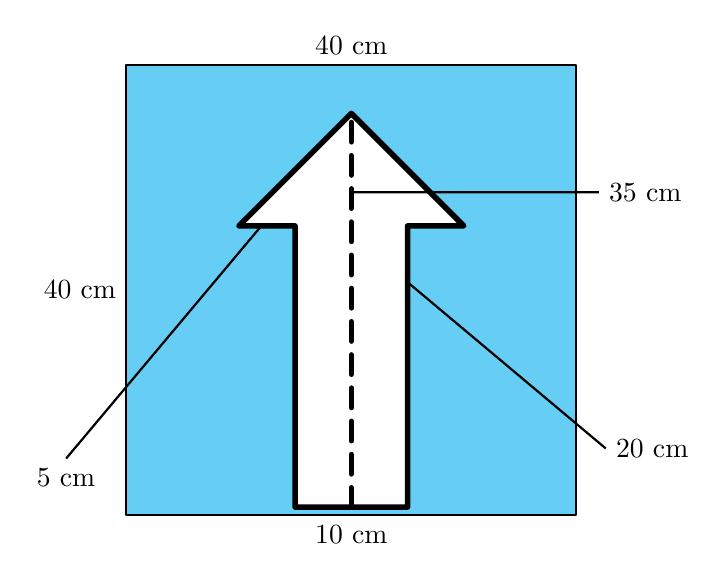
\begin{tikzpicture}[scale=1,line width=0.8pt,line join=round,>=stealth]
			\def\a{7}
			\path (0,0) coordinate (A)
			(0,35/\a) coordinate (B)
			;
			\draw[fill=cyan!60] (-20/\a,-0.1) -- (-20/\a,40/\a-0.1)node[midway,left]{40 cm} -- (20/\a,40/\a-0.1)node[midway,above]{40 cm}--(20/\a,-0.1)-- cycle node[midway,below]{10 cm};
			\draw[fill=white,line width=2pt] (0,35/\a)--++(10/\a,-10/\a)--++(180:5/\a)--++(-90:25/\a)--++(180:10/\a)--++(90:25/\a)--++(180:5/\a)--cycle;
			\draw[dash pattern=on 7pt off 5pt,line width=2pt,line cap=round] (0,0)--(90:35/\a);
			\draw[thick] (0,28/\a)--++(0:22/\a)node[right]{35 cm}
			(-8/\a,25/\a)--++(-130:27/\a)node[below]{5 cm}
			(5/\a,20/\a)--++(-40:23/\a)node[right] {20 cm};
		\end{tikzpicture}
	\end{center}
	\loigiai{$1250$ $m^2$}
\end{bt}


  
\Closesolutionfile{ansbook} 
\newpage
		
%%%%%%%%%%%%%% ĐỀ SỐ 17
\Opensolutionfile{ansbook}[ans/ansD17] 
\section{ĐỀ SỐ \thesection } %%Đề 17 
\setcounter{bt}{0}

%%Câu 1.
\begin{bt} Thực hiện phép tính:
	\begin{listEX}[3]
	\item $15\cdot 113+85\cdot 15+15\cdot 2$;
 	\item$6\cdot 10^3+7\cdot 10^2+8$;
  	\item$3-\left\{24:\left[26-\left(18: 9+12\cdot 1^{2019}\right)\right]\right\}$.
\end{listEX}
	
	\loigiai{a) $3000$ \hfill b) $6708$ \hfill c) $1$. 	}
\end{bt}

%%Câu 2.
\begin{bt} Tìm x biết
	
	\begin{listEX}[3]
		\item $3 x+12=6^2$;
		\item $(x-3): 5=103$;
		\item $65-4^{x-3}=2020^0$.
	\end{listEX}
	
	\loigiai{a) $x=8$ \hfill b) $x=518$ \hfill c) $x=6$.}
\end{bt}



%%Câu 3.
\begin{bt}
	\
	\begin{listEX}
		\item Tìm ước chung lớn nhất của 45, 120 và 270.
		\item Hưởng ứng chương trình Sữa học đường với chủ đề "Chung tay vì một Việt Nam vươn cao", công ty sữa ABC cần phân phối đến một trường học số hộp sữa nằm trong khoảng từ 600 đến 800 hộp và nếu đóng số hộp trên thành các thùng 12 hộp, thùng 16 hộp, thùng 20 hộp thì vừa đủ. Tính số hộp sữa công ty ABC cần phân phối.
		
	\end{listEX}
	
	\loigiai{a) $15$ \hfill b) $720$.
	}
\end{bt}



%%Câu 4.
\begin{bt}
Ô nhiễm môi trường đang là vấn đề cấp bách hiện nay và có nhiều phương án để khắc phục, giảm thiểu hậu quả. Trong đó phổ biến là việc thực hiện 3R (Reduce: giảm thiểu, Reuse: sử dụng lại, Recycle: tái chế) đang được áp dụng tại một số nước trong đó có Việt Nam. Theo đó, một trường trung học cơ sở đã phát động phong trào thu gom chất thải qua sử dụng với bảng điểm quy đổi như sau:
\begin{center}
\begin{tabular}{|c|c|c|c|}
	\hline \bf Chất thải & \bf Đơn vị & \bf Số lượng & \bf Điểm quy đổi \\
	\hline Giấy & kg & 2 & 5 \\
	\hline Hộp sữa & hộp & 50 & 2 \\
	\hline Pin & viên & 5 & 2 \\
	\hline
\end{tabular}
\end{center}
Lớp 6C nộp được 84 kg giấy, 925 hộp sữa và 30 viên pin. Hỏi lớp 6C quy đổi được bao nhiêu điểm?
	\loigiai{259 điểm.}
\end{bt}


%%Câu 5.
\begin{bt}
Sân chơi nhà bạn Hùng hình chữ nhật có chiều dài 20 m, chiều rộng 12 m. Giá mỗi viên gạch hình vuông cạnh 80 cm là $200\,000$ đồng, giá mỗi viên gạch hình vuông cạnh 50 cm là $50\,000$ đồng. Tiền công thợ lát nền gạch hình vuông cạnh 80 cm là $20\,000$ đồng/m$^2$. Tiền công thợ lát nền gạch hình vuông cạnh 50 cm là $25\,000$ đồng/m$^2$. Hỏi nhà bạn Hùng chọn phương án nào sẽ đỡ chi phí hơn: lát gạch hình vuông cạnh 80 cm hay lát gạch hình vuông cạnh 50 cm?
	
	\loigiai{
			Nhà bạn Hùng chọn phương án lát gạch 50 cm sẽ đỡ chi phí hơn.}
\end{bt}


%%Câu 6.
\begin{bt}
	Bạn An có ngày sinh là số nguyên tố lớn nhất nhỏ hơn 30.\\
	Tháng sinh của bạn là số nguyên tố nhỏ nhất.\\
	Năm sinh của bạn có dạng $\overline{200^*}$ chia hết cho 2 và chia 5 dư 3.
	\begin{listEX}
		\item Hãy tìm ngày tháng năm sinh của bạn An.
		\item 	Nếu mỗi năm bạn An đều được tổ chức sinh nhật thì có thể tổ chức sinh nhật đúng ngày sinh của mình không? Vì sao?
	\end{listEX}
	
	\loigiai{
	a) An sinh ngày $29$ tháng $2$ năm $2008$. \hfill b) Không vì năm nhuận mới có.
	}
\end{bt}


%%Câu 7.
\begin{bt}
	
	Tìm $x, y$ biết: $\overline{1 x y}$ là bội của 9 và $x$ là số nguyên tố lẻ nhỏ nhất.
	

	\loigiai{ 	Vậy số cần tìm là $135$  }
\end{bt}  
\Closesolutionfile{ansbook} 
\newpage
	
%%%%%%%%%%%%%% ĐỀ SỐ 18
\Opensolutionfile{ansbook}[ans/ansD18] 
\section{ĐỀ SỐ \thesection }%ĐỀ 6
\setcounter{bt}{0}

%%Câu 1.
\begin{bt} \textbf{ } 
	\begin{listEX}
		\item Em hãy tìm: ƯCLN$(108,60)$.
		\item Sắp xếp các số nguyên sau theo thứ tự giảm dần: $-20\,623 ;\ 0 ;\ 15 ;\ -20 ;\ 7 ;\ -99$
		\item Một kho đông lạnh đang ở nhiệt độ là $-5^{\circ}$C. Sau đó, một công nhân đã bấm nút điều chỉnh tăng nhiệt độ trong kho lên $8^{\circ} \mathrm{C}$. Hỏi nhiệt độ trong kho đông lạnh lúc này là bao nhiêu?
	\end{listEX}
	
	\loigiai{a) ƯCLN$(108, 60) = 12$ \hfill b) $15, 7, 0, -20, -99, -2023$ \hfill c) $3^{\circ} C$
	}
\end{bt}


%%Câu 2. 
\begin{bt} \textbf{ }
	\begin{listEX}[2]
		\item $43+(-100)+(-43)+150$;
		\item $5^{2022}:5^{2019}-[130-(12-2.3)^2]$;
		\item $S = -1+3-5+7-9+11-...-201+203$.
	\end{listEX}
	\loigiai{a) $50$ \hfill b) $31$ \hfill c) $202$.
	}
\end{bt}




%%Câu 3.
\begin{bt} Tìm số tự nhiên $x$ biết:
	\begin{listEX}[3]
		\item $2x + 15 = 57$;
		\item $100 - (x + 15) = 150$;
		\item $x \in \text{B}(12)$ và $40 < x \leqslant 50$.
	\end{listEX}
	
	\loigiai{a) $21$ \hfill b) $-65$ \hfill c) $48$}
\end{bt}


%%Câu 4.
\begin{bt} Một trường trung học cơ sở trên địa bàn TP HCM tổ chức cho tất cả các em học sinh của mình đi tham quan, hướng nghiệp. Khi xếp hàng $8$ em, hàng $10$ em, hàng $12$ em để học sinh tham gia các trò chơi trải nghiệm ngoài trời thì không thừa và không thiếu bạn nào. Hỏi trường đó có tất cả bao nhiêu học sinh, biết rằng tổng số học sinh của trường đó khoảng từ $400$ đến $500$ em.
	
	\loigiai{$480$ học sinh}
\end{bt}


%%Câu 5.
\begin{bt} Một cửa hàng A thống kê số lượng cam bán được trong $4$ ngày cuối tuần vừa rồi bằng biểu đồ tranh sau đây:
	\begin{center}
		\def\icon{\tikz{
				\fill[orange] (0,0) circle (0.4);
				\fill[white] (0,0) circle (0.35) (0,0) circle (0.2cm);
				\fill[orange!60!yellow] (0,0) circle (0.29);
				\foreach \angle in {0,45,...,315} { \draw[white, line width=1pt] (0,0) -- (\angle:0.29);}
		}}
		\def\hicon{\tikz{\clip(-0.4,-0.4)rectangle(0,0.4);\fill[orange] (0,0) circle (0.4);
				\fill[white] (0,0) circle (0.35) (0,0) circle (0.2cm);
				\fill[orange!60!yellow] (0,0) circle (0.29);
				\foreach \angle in {0,45,...,315} { \draw[white, line width=1pt] (0,0) -- (\angle:0.29);}}}
		\def\vetranh#1{\foreach \dem in{1,...,#1}{\icon \ }}{
			\begin{tabular}{|c|p{7cm}<{}|}\hline 
				\multicolumn{2}{|c|}{\bf Số lượng cam bán được trong 4 ngày cuối tuần vừa rồi của cửa hàng A }\\  \hline 
				Thứ Năm &\vetranh{5}\\ \hline 
				Thứ Sáu&\vetranh{3}\ \hicon  \\ \hline 
				Thứ Bảy&\vetranh{4} \\ \hline 
				Chủ nhật &\vetranh{7} \\ \hline 
			\end{tabular}\\
			Biết rằng: \icon = 10 kg;        \hicon = 5 kg}
	\end{center}     
	\begin{enumerate}
		\item Lập bảng thống kê tương ứng với biểu đồ tranh trên.
		\item Từ bảng thống kê, em hãy cho biết: 
		\begin{itemize}
			\item Thứ mấy cửa hàng đó bán được ít cam nhất?
			\item Tổng số cam bán được trong 4 ngày cuối tuần vừa rồi là bao nhiêu kg?
		\end{itemize} 
	\end{enumerate}
	
	
	
	
	\loigiai{a) Học sinh tự lập bảng \hfill b) Thứ $6$; $195$kg
	}
\end{bt}

%%Câu 6.
\begin{bt} 	Một khu đất của ông Tám có dạng như hình vẽ bên:
	\immini{			
		\begin{listEX}
			\item Tính chu vi của khu đất nhà ông Tám.
			\item Ông Tám mua thêm một miếng đất hình vuông liền kề với khu đất của ông có kích thước cạnh bằng $400$ cm. Sau đó, ông dùng những viên gạch hình bình hành lát nền toàn bộ đất của ông với chi phí mua gạch là $7$ triệu đồng. Em hãy tính diện tích một viên gạch hình bình hành này là bao nhiêu dm$^{2}$, biết rằng giá $1$ thùng gạch (gồm $12$ viên) là $168\,000$ đồng và khoảng cách giữa các viên gạch là không đáng kể.
		\end{listEX}
	}{
		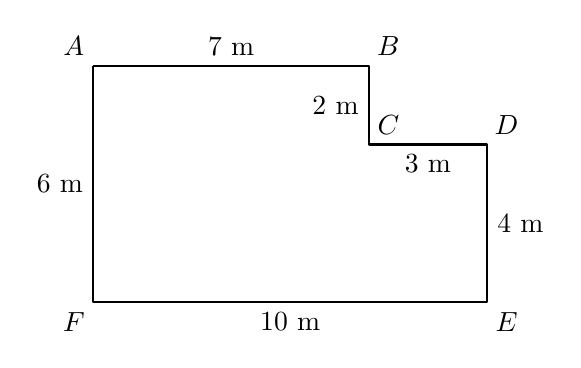
\begin{tikzpicture}[scale=1,line width=0.8pt,line join=round,>=stealth]
			\def\a{2}
			\path (0,0) coordinate (F)
			(0,6/\a) coordinate (A)
			(7/\a,6/\a) coordinate (B)
			(7/\a,4/\a) coordinate (C)
			(10/\a,4/\a) coordinate (D)
			(10/\a,0) coordinate (E)
			;
			\draw (A)--(B)node[midway,above]{7 m}
			--(C)node[midway,left]{2 m}
			--(D)node[midway,below]{3 m}
			--(E)node[midway,right]{4 m}
			--(F)node[midway,below]{10 m}
			--(A)node[midway,left]{6 m}
			;
			\foreach \x/ \goc in {A/135,B/45,C/45,D/45,E/-45,F/-135}  \fill (\x) circle (0pt)        
			($(\x)+(\goc:3.5mm)$) node {$\x$};
		\end{tikzpicture}
	}
	\loigiai{a) $32$ m \hfill b) $14$ dm$^2$
	}
\end{bt}


%%Câu 7.
\begin{bt} Tìm số nguyên tố $n$ sao cho $(3n+7)$ là bội của $(n+1)$.   
	
	\loigiai{$n = 3$}
\end{bt}  
\Closesolutionfile{ansbook} 
\newpage

%%%%%%%%%%%%%% ĐỀ SỐ 19
\Opensolutionfile{ansbook}[ans/ansD19] 
\section{ĐỀ SỐ \thesection}%ĐỀ 1 
\setcounter{bt}{0}
%%Câu 1.
\begin{bt} Thực hiện các phép tính:
	\begin{listEX}[2]
		\item $-2-(-12)+(-18)$;
		\item $126^{15}: 126^{14}-26 \cdot(40-38)^{2}$.
	\end{listEX}
	\loigiai{a) $-8$ \hfill b) $22$.
	}
\end{bt}

%%Câu 2.
\begin{bt} Nhiệt độ ban đầu trong một kho lạnh là $-20^{\circ} \mathrm{C}$. Do yêu cầu bảo quản hàng hóa, người quản lý kho tiếp tục giảm $3^{\circ} \mathrm{C}$. Sau đó, do hàng hóa được lấy bớt nên quản lý kho tăng nhiệt độ thêm $5^{\circ} \mathrm{C}$. Hỏi sau khi tăng, nhiệt độ hiện tại của kho lạnh là bao nhiêu?
	
	\loigiai{$-18^\circ$C.}
\end{bt}


%%Câu 3.
\begin{bt}  Một đội nghi thức của một trường Trung học cơ sở A có khoảng $100$ đến $150$ đội viên đã tham gia hội thi "Nghi thức Đội". Khi tham gia biểu diễn, đội xếp đội hình $10$ hàng, $12$ hàng, $15$ hàng đều vừa đủ. Hỏi đội nghi thức của trường Trung học cơ sở A có bao nhiêu đội viên tham gia hội thi?
	\loigiai{$120$ đội viên.}
\end{bt}


%%Câu 4.
\begin{bt} \textbf{ }\\
	\begin{minipage}[h]{0.5\linewidth}
		Biểu đồ tranh ở hình bên cho ta thông tin về loại nhạc cụ yêu thích của các bạn học sinh khối lớp 6 của trường Trung học cơ sở A. Biết rằng không có học sinh không thích nhạc cụ.
		\begin{listEX}
			\item Số lượng học sinh yêu thích nhạc cụ Organ nhiều hơn số học sinh yêu thích nhạc cụ trống là bao nhiêu?
			\item Tính tổng số học sinh của trường Trung học cơ sở A.
		\end{listEX}
	\end{minipage}
	\begin{minipage}{0.5\linewidth}
		\begin{center}
			\def\icon{\huge \quarterNote}
			\def\hicon{\huge \eighthNote}
			\def\vetranh#1{\foreach \dem in{1,...,#1}{\icon \ }}{
				\begin{tabular}{|c|p{4cm}<{}|}\hline 
					\bf Loại nhạc cụ&\multicolumn{1}{c|}{\bf Số học sinh yêu thích}\\ \hline 
					Organ &\vetranh{4}\ \hicon \\ \hline 
					Ghi ta &\vetranh{5}\ \hicon  \\ \hline 
					Kèn &\vetranh{2}\ \hicon \\ \hline 
					Trống &\vetranh{4} \\ \hline 
					Sáo &\vetranh{2}\ \hicon \\ \hline 
				\end{tabular}\\
				(\icon \normalsize = 10 học sinh;        \hicon \normalsize = 5 học sinh)}	
		\end{center}
		
	\end{minipage}
	\loigiai{a) $5$ học sinh \hfill b) $190$ học sinh.
	}
\end{bt}


%%Câu 5.
\begin{bt} 
	\immini[thm]{
		Một bồn hoa hình chữ nhật (như hình vẽ), có \\
		$AB = HF = 4$ m, $BC = EG = 3$ m. Người ta trồng hoa hồng bên trong phần đất hình thoi $HEFG$, phần đất còn lại trồng hoa mười giờ.
		\begin{listEX}
			\item Tính diện tích đất trồng hoa hồng?
			\item Tính diện tích đất trồng hoa mười giờ?
		\end{listEX}
	}{
		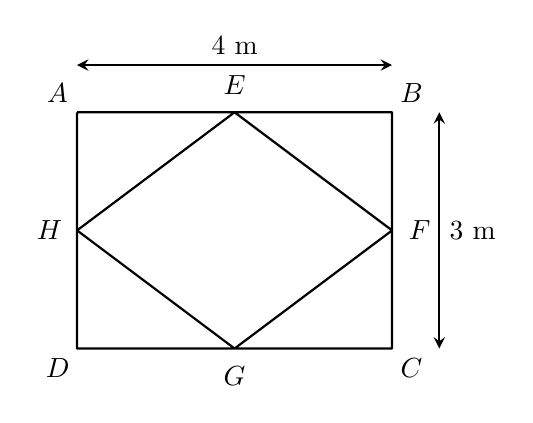
\begin{tikzpicture}[scale=1,line width=0.8pt,line join=round,>=stealth]
			\def\a{4} \def\b{3} 
			\path (0,0) coordinate (D)
			(0,\b) coordinate (A)
			(\a,\b) coordinate (B)
			(\a,0) coordinate (C)
			($(A)!0.5!(B)$) coordinate (E)
			($(B)!0.5!(C)$) coordinate (F)
			($(C)!0.5!(D)$) coordinate (G)
			($(A)!0.5!(D)$) coordinate (H)
			;
			\draw (A)--(B)--(C)--(D)--(A)
			(E)--(F)--(G)--(H)--(E)
			;
			\draw[<->] (A)++(90:0.6)--++(0:\a)node[midway,above]{4 m};
			\draw[<->] (B)++(0:0.6)--++(-90:\b)node[midway,right]{3 m};
			\foreach \x/ \goc in {A/135,B/45,C/-45,D/-135,E/90,F/0,G/-90,H/180}  \fill (\x) circle (0pt)        
			($(\x)+(\goc:3.5mm)$) node {$\x$};
		\end{tikzpicture}
	}
	\loigiai{a) $6$ m$^2$ \hfill b) $6$ m$^2$.}
\end{bt}


%%Câu 6. 
\begin{bt} Chứng minh: $\left(7+7^{2}+7^{3}+7^{4}+\ldots+7^{48}+7^{49}+7^{50}+7^{51}\right)$ chia hết cho $399$.
	
	\loigiai{HD: Nhận thấy $(7+7^{2}+7^{3})$ $\vdots$ $399$\\
		Dùng phương pháp kết hợp và tính chất phân phối của phép nhân đối với phép cộng.}
\end{bt}
   
\Closesolutionfile{ansbook} 
\newpage

%%%%%%%%%%%%%% ĐỀ SỐ 20
\Opensolutionfile{ansbook}[ans/ansD20] 
\section{ĐỀ SỐ \thesection } %Đề 20
\setcounter{bt}{0}

%%Câu 1.
\begin{bt} \textbf{ }
	\begin{enumerate}
		\item Tìm tất cả các ước của $-18$.
		\item Tìm số tự nhiên $x$ biết $x\ \vdots \ 28$, $x \ \vdots \ 8$ và $x<300$.
		\item Sắp xếp các số nguyên sau theo thứ tự tăng dần: $2000;-201;0;-199;2024$. 
	\end{enumerate}
	\loigiai{\begin{listEX}[2]
		\item  Ư$(-18)=\{\pm1;\pm2;\pm3;\pm6;\pm9;\pm18\}$ 
		\item $x\in\{0;56;112;168;224;280\}$ 
		\item $-201;-199;0;2000;2024$
		\end{listEX}	}
\end{bt}


%%Câu 2.
\begin{bt} Tính toán hợp lý (nếu có thể):
	\begin{listEX}[2]
			\item $28\cdot(-63)+28\cdot(-37)+800$;
			\item $(-24):(-2)^3+38:(15+4)$;
			\item $400+150:\left( 2^{30}:2^{25}-3^3\right)  $;
			\item $10+\left[ \left( 8^2-48\right) \cdot5+\left( 2^2\cdot10+8\right) \right] :2^4$.
	\end{listEX}
	\loigiai{a) $-2000$ \hfill b) $5$ \hfill c) $430$ \hfill d) $18$.
	}
\end{bt}



%%Câu 3.
\begin{bt} Tìm số nguyên $x$, biết:
	\begin{listEX}[2]
			\item $52:x=-4$;
			\item $(x+7)-15^0=202-19$;
			\item $2^{x+1}\cdot5-8=72$;
			\item $(2x+5)(5^3-123)=-30$.
	\end{listEX}
	\loigiai{a) $x=-13$ \hfill b) $x=177$ \hfill c) $x=3$ \hfill d) $x=-10$.
	}
\end{bt}


%%Câu 4.
\begin{bt} Điểm kiểm tra thường xuyên môn Anh văn của học sinh lớp 6A được cho bởi bảng thống kê sau:
	\begin{center}
		\begin{tabular}{|c|c|c|c|c|c|c|c|c|c|}\hline
			\textbf{Điểm số}&2&3&4&5&6&7&8&9&10 \\ \hline
			\textbf{Số học sinh}&2&1&3&4&5&3&6&8&4 \\ \hline
		\end{tabular}\\
	\end{center}
	\begin{enumerate}
		\item Lớp 7A có tổng cộng bao nhiêu học sinh? 
		\item Điểm số nào có số học sinh đạt được ít nhất? Điểm số nào có số học sinh đạt được nhiều nhất?
		\item Có bao nhiêu học sinh đạt từ điểm 8 trở lên? Chiếm tỷ lệ bao nhiêu phần trăm?
	\end{enumerate}
	\loigiai{a) Có $36$ học sinh \hfill b) Ít nhất: $3$ điểm, nhiều nhất: $9$ điểm \hfill c) Có $18$ học sinh, chiếm $50\%$
	}
\end{bt}


%%Câu 5.
\begin{bt} \immini{Điền các số $ -1$, $ -2$, $-3$, $-4$, $5$, $ 6$, $7$ vào các vòng tròn trên sao cho 
	tổng của ba số nằm trên cùng một hàng thẳng đều bằng $0$.}{
	
\begin{tikzpicture}[thick,scale=0.5]
		\def\R{2.2}
		\def\r{8mm}
		
		% 6 vòng tròn ngoài
		\foreach \a in {90,30,-30,-90,-150,150}{
			\draw (\a:\R) circle (\r);
		}
		% vòng tròn tâm
		\draw (0,0) circle (\r);
		
		
	\end{tikzpicture}}
	\loigiai{
		\text{}
		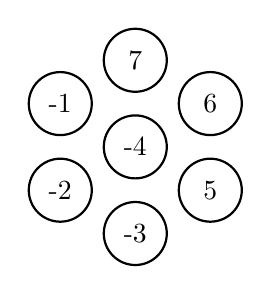
\begin{tikzpicture}[thick,scale=0.5]
			\def\R{2.2}
			\def\r{8mm}
			
			% 6 vòng tròn ngoài
			\foreach \a in {90,30,-30,-90,-150,150}{
				\draw (\a:\R) circle (\r);
			}
			% vòng tròn tâm
			\draw (0,0) circle (\r);
			
			% điền số
			\node at (90:\R) {7};
			\node at (30:\R) {6};
			\node at (-30:\R) {5};
			\node at (-90:\R) {-3};
			\node at (-150:\R) {-2};
			\node at (150:\R) {-1};
			\node at (0,0) {-4};
	\end{tikzpicture}}
\end{bt}



%%Câu 6.
		\begin{bt} 
			\immini[thm]{Một mảnh vườn hình chữ nhật có chiều dài 35 m, chiều rộng là 25 m với lối đi hình bình hành rộng 4 m.
			\begin{enumerate}
				\item Tính diện tích miếng đất hình chữ nhật. 
				\item Tính diện tích phần mảnh vườn không tính lối đi.
			\end{enumerate}
		}{
		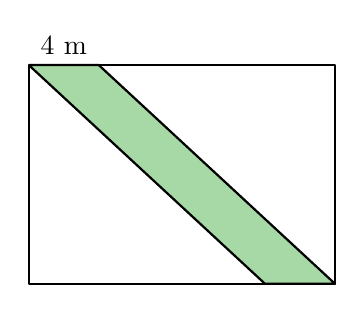
\begin{tikzpicture}[scale=1,line width=0.8pt,line join=round,>=stealth]
			\def\s{9}
			\draw[fill=white] (0,0) rectangle (35/\s,25/\s);
			\draw[fill=green!40!gray!50] (0,25/\s)--(27/\s,0)--(35/\s,0)--(8/\s,25/\s)--(0,25/\s)node[midway,above]{4 m};
			\end{tikzpicture}
		}
			\loigiai{a) $875$ m$^2$ \hfill b) $775$ m$^2$.}
		\end{bt}
		

%%Câu 7.
\begin{bt} Tìm số nguyên $x$ để $(2x+3)\,\vdots\,(x-1)$.
	\loigiai{$n\in\{2;0;6;-4\}$}
\end{bt}  
\Closesolutionfile{ansbook} 
\newpage


 


%%%%%%%%%%%%%% ĐỀ SỐ 21
\Opensolutionfile{ansbook}[ans/ansD21] 	
\section{ĐỀ SỐ \thesection } %star6
\setcounter{bt}{0}

%%Câu 1.
\begin{bt} Thực hiện phép tính:
		\begin{listEX}[2]	
			\item $354 + 307 + 46 + 193$;
			\item $375 : \left\{ 32 - \left[ 4 + (5 \cdot 3^2 - 42) \right] \right\} - 14$;
			\item $3^5 \cdot 108 - 3^5 \cdot 107 + 9^2 \cdot 3$;
			\item $4^3 \cdot 5 - 200 : 5^2 + 2023^0$.
		\end{listEX}
	\loigiai{a) $900$ \hfill b) $1$ \hfill c) $486$ \hfill d) $313$.}
\end{bt}


%%Câu 2.
\begin{bt} Tìm số nguyên $x$, biết:
		\begin{listEX}[2]
		 \item $x - 48 : 16 = 37 \cdot 2$;
		\item $6(x + 2^3) + 40 = 100$;
		\item $3(x + 10) - 15 = 19+x$;
		\item $2^{x+1}+5^2\cdot 2^x=2^3\cdot 3^3$.
		\end{listEX}
	\loigiai{a) $x = 77$ \hfill b) $x = 2$ \hfill c) $x = 2$ \hfill d) $x = 3$.
	}
\end{bt}


%%Câu 5.
\begin{bt} Một rạp xiếc khuyến mãi giảm giá $5\%$ cho vé người lớn và $15\%$ cho vé trẻ em. Biết giá niêm yết của vé trẻ em là $60\,000$ đồng.
	\begin{listEX}
		\item Tính giá vé trẻ em sau khi được giảm giá; 
		\item Biết giá sau khi giảm của vé người lớn là $123\,500$ đồng. Hãy tính giá niêm yết của vé người lớn
	\end{listEX}
	\loigiai{
		a) $51\,000$ đồng \hfill b) $130\,000$ đồng
		}
\end{bt}


%%Câu 3.
\begin{bt} Ba ô tô cùng khởi hành một lúc từ một bến. Thời gian cả đi lẫn về của xe thứ nhất là $40$ phút, của xe thứ hai là $50$ phút, của xe thứ ba là $30$ phút. Khi trở về bến, mỗi xe đều nghỉ $10$ phút rồi tiếp tục chạy. Hỏi sau ít nhất bao lâu:
	\begin{listEX}[2]
	 \item Xe thứ nhất và xe thứ hai cùng rời bến?
	\item Xe thứ hai và xe thứ ba cùng rời bến?
	\item Cả ba xe cùng rời bến?
	\end{listEX}
	\loigiai{ 
	a) $5$ giờ \hfill b) $2$ giờ \hfill c) $10$ giờ	}
\end{bt}


%%Câu 4.
\begin{bt} Để phòng dịch Covid-19, xã ABC thành lập các đội phản ứng nhanh gồm bác sĩ và điều dưỡng viên. Ban đầu có $45$ bác sĩ và $55$ điều dưỡng viên đăng kí. Khi chia đội thực tế có thêm $3$ bác sĩ đăng kí tham gia và có $1$ điều dưỡng viên bị nhiễm Covid-19 nên không tham gia. Hỏi có thể thành lập được nhiều nhất bao nhiêu đội phản ứng nhanh? Khi đó mỗi đội có bao nhiêu bác sĩ và bao nhiêu điều dưỡng viên?
	\loigiai{ $6$ đội; mỗi đội $8$ bác sĩ và $9$ điều dưỡng viên.}
\end{bt}



\begin{bt} Nhà thi đấu Phú Thọ có sàn hình chữ nhật, chiều dài $130$ m và chiều rộng $105$ m. 
	\begin{listEX}
		\item Tính diện tích sàn xây dựng của nhà thi đấu Phú Thọ;
		\item Người ta lát sàn bằng gạch hình vuông cạnh $60$ cm. Tính số thùng gạch cần để lát hết sàn, biết hao hụt khi thi công là $5\%$ số gạch và mỗi thùng có $50$ viên gạch.
	\end{listEX}
	\loigiai{a) $13\,650$ m$^2$ \hfill b) $797$ thùng
	}
\end{bt}



\begin{bt}Kết quả điều tra về loại quả ưa thích nhất của một số bạn trong lớp được ghi như bảng 
\begin{center}
		\begin{tabular}{|c|c|c|c|}

		\hline
		Cam & Ổi & Chuối & Xoài \\ \hline
		Khế & Cam & Ổi & Khế \\ \hline
		Xoài & Ổi & Chuối & Xoài \\ \hline
		Xoài & Cam & Khế & Cam \\ \hline
		Ổi & Khế & Xoài & Chuối \\ \hline
	\end{tabular}
\end{center}
	\begin{listEX}
		\item Có bao nhiêu bạn tham gia trả lời?
		\item Hãy lập bảng thống kê và cho biết loại quả nào được yêu thích nhất; loại quả đó chiếm bao nhiêu phần trăm so với tổng số bạn
	\end{listEX}
	\loigiai{
		\begin{listEX}
			\item   $20$ bạn tham gia
			\item Thống kê tần số và tỉ lệ:
			
			\begin{center}
				\begin{tabular}{|c|c|c|}
					\hline
					\textbf{Loại quả} & \textbf{Số bạn} & \textbf{Tỉ lệ} \\ \hline
					Cam & $4$ & $20\%$ \\ \hline
					Ổi & $4$ & $20\%$ \\ \hline
					Chuối & $3$ & $15\%$ \\ \hline
					Xoài & $5$ & $25\%$ \\ \hline
					Khế & $4$ & $20\%$ \\ \hline
					\textbf{Tổng} & $20$ & $100\%$ \\ \hline
				\end{tabular}
			\end{center}
			
			Vậy quả được yêu thích nhất là Xoài, chiếm $25\%$ tổng số bạn
	\end{listEX}}
\end{bt}

\begin{bt} 
	Tìm số tự nhiên có năm chữ số, biết rằng nếu viết thêm chữ số $2$ vào đằng sau số đó thì được số lớn gấp ba lần số có được bằng cách viết thêm chữ số $2$ vào đằng trước số ban đầu.
	\loigiai{
		Gọi số phải tìm là $\overline{abcde} = x$ \quad ($a,b,c,d,e \in \mathbb{N}$; $a \ne 0$; $a,b,c,d,e \le 9$).
		Khi đó:
		\begin{align*}
			\overline{abcde2} &= 3 \cdot \overline{2abcde} \\
			10x + 2 &= 3\cdot(200000 + x) \\
			x &= 85714.
		\end{align*}
		
	}
\end{bt}
  
\Closesolutionfile{ansbook} 
\newpage

%%%%%%%%%%%%%% ĐỀ SỐ 22
\Opensolutionfile{ansbook}[ans/ansD22] 	

\section{ĐỀ SỐ \thesection } %star7
\setcounter{bt}{0}
%%%%%%%%%%%%%%% BÀI 1
\begin{bt} Thực hiện phép tính (tính hợp lí nếu có thể)
	\begin{listEX}[2]
		\item  $A=2025\cdot2026-2025^2$;
        \item $B=3^{2025}:9^{1012}-3\cdot3^2$;
        \item $C=(-2025)-23 +2025+73$;
        \item $D=( -900): \{400+[ (-7)^2+ 1]\} +2025^0$.
	\end{listEX}

	
\loigiai{a) $A=2025$ \hfill b) $B=-24$ \hfill c) $C=50$ \hfill d) $D=-1$
}
\end{bt}

%%%%%%%%%%%%%%% BÀI 2
\begin{bt} Tìm sso nguyên $x$
	\begin{listEX}[2]
		\item  $ x+135=280$;
		\item $3.|2x+3|=201$;
        \item $ 15-5\cdot[(x-30)+6^2]=-20$;
        \item $4^{x+1}+2^2=1028.
$
	\end{listEX}
	\loigiai{
            a) $x=145$;\hspace{1 cm}  
            b) $x=-35$ hay $x=32$; \hspace{1 cm}   
            c) $x=1$;  \hspace{1 cm}   
            d)$x=4$;   \hspace{1 cm}    }
\end{bt}



%%%%%%%%%%%%%%% BÀI 3
\begin{bt}%[Đề bài tự luận]
	Số học sinh khối 6 của trường Ngôi Sao khi xếp hàng $10$ em thì thừa $8$ em,  
	xếp hàng $12$ em thì thừa $10$ em,  
	khi xếp hàng $15$ em thì thừa $13$ em nhưng khi xếp hàng $17$ em thì vừa đủ.  
	
	Tính số học sinh khối 6 của trường, biết rằng số học sinh là một số tự nhiên có $3$ chữ số và nhỏ hơn $250$.
	\loigiai{$60$ ngày}
\end{bt}

%%%%%%%%%%%%%%% BÀI 4
\begin{bt} Hai bạn Lan và Điệp cùng học chung một trường THCS nhưng ở hai lớp khác nhau. An cứ 10 ngày lại trực nhật, Điệp cứ 12 ngày lại trực nhật. Lần đầu tiên hai bạn trực nhật vào cùng một ngày. Hỏi sau ít nhất bao nhiêu ngày hai bạn lại cùng trực nhật? 
 \loigiai{
It nhất sau 60 ngày hai bạn lại cùng trực nhật vào 1 ngày. 
}

\end{bt}
%%%%%%%%%%%%%%% BÀI 5
\begin{bt} 
Một mảnh vườn hình chữ nhật (như hình bên) có chiều dài 9m, chiều rộng 7m. Người ta chia mảnh vườn thành bốn khu gồm hai khu hình vuông cạnh 3m, hai khu hình chữ nhật có chiều dài 5m, chiều rộng 3m và chừa lại phần lối đi như hình bên.
\begin{center}
	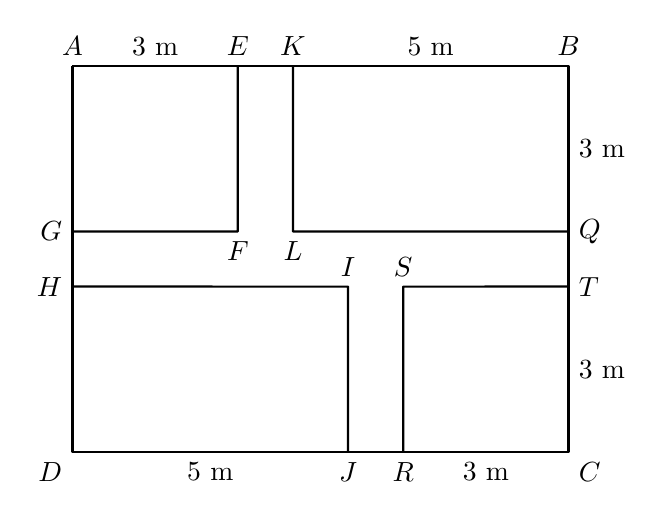
\begin{tikzpicture}[scale=0.7,line width=0.8pt,line join=round,>=stealth]
		\draw (0,0)coordinate[label=above:$A$](A)--(3,0)coordinate[label=above:$E$](E)--(4,0)coordinate[label=above:$K$](K)--(9,0)coordinate[label=above:$B$](B)--(9,-3)coordinate[label=right:$Q$](Q)--(9,-4)coordinate[label=right:$T$](T)--(9,-7)coordinate[label=below right:$C$](C)--(6,-7)coordinate[label=below:$R$](R)--(5,-7)coordinate[label=below:$J$](J)--(0,-7)coordinate[label=below left:$D$](D)--(0,-4)coordinate[label=left:$H$](H)--(0,-3)coordinate[label=left:$G$](G)--(A);
		\draw (G)--(3,-3)coordinate[label=below:$F$](F)--(E) (K)--(4,-3)coordinate[label=below:$L$](L)--(Q) (T)--(6,-4)coordinate[label=above:$S$](S)--(R) (J)--(5,-4)coordinate[label=above:$I$](I)--(H);
		\draw ($(A)!.5!(E)$) node[above]{$3$ m}
		($(K)!.5!(B)$) node[above]{$5$ m}
		($(B)!.5!(Q)$) node[right]{$3$ m}
		($(T)!.5!(C)$) node[right]{$3$ m}
		($(R)!.5!(C)$) node[below]{$3$ m}
		($(D)!.5!(J)$) node[below]{$5$ m};
	\end{tikzpicture}
\end{center}
 \begin{listEX}
     \item Tính diện tích phần lối đi.
     \item Người ta muốn lát gạch toàn bộ lối đi bằng những viên gạch hình vuông có cạnh bằng 50cm, biết mỗi viên gạch có giá 25 000 đồng. Tính số tiền cần mua gạch để lát hết lối đi đó.
     \item Trên mảnh vườn, người ta trồng tắc thì thu được 25 000 đồng/$m^2$, trồng quýt thì được 30 000 đồng/$m^2$, trồng cam thì được 40 000 đồng/$m^2$. Em hãy chọn phương có doanh thu tốt hơn trong 2 phương án sau:
\\\textbf{Phương án 1:} Trồng quýt trên cả mảnh đất (trừ lối đi).
\\\textbf{Phương án 2:} Trồng tắc trên mảnh đất hình chữ nhật và trồng cam trên mảnh đất hình vuông. 
\end{listEX}

 
 \loigiai{
 a) $15$ m$^2$ \hfill b) $1\,500\,000$ đồng \hfill c) Phương án 2.}\end{bt}
 %%%%%%%%%%%%%%% BÀI 6
\begin{bt} 
Cho biểu đồ cột cho biết thông tin về kết quả học tập của học sinh khối 6 của  trường Star. Từ biểu đồ em hãy cho biết:
\begin{listEX}
\item Số học sinh xếp loại học lực giỏi là bao nhiêu học sinh? Số học sinh xếp loại học lực giỏi ít hơn số học sinh xếp loại học lực khá bao nhiêu học sinh?
\item Khối 6 có tất cả bao nhiêu học sinh? 
\end{listEX}
     \begin{center}
          	\begin{tikzpicture}[scale=0.7,font=\small,line join=round,>=stealth]
         		% Kích thước khung vẽ
         		\def\hoanh{10.5}
         		\def\tung{6.8}
         		\def\cotwidth{0.7} % độ rộng cột
         		
         		% Tiêu đề
         		\node[above] at (\hoanh/2,\tung+1.2){\normalsize \bfseries Xếp loại học lực học sinh khối 6};
         	 ;
         		
         		% Trục
         		\draw[->] (0,0) node[left]{0} -- (\hoanh,0);
         		\draw[->] (0,0) -- (0,\tung+0.8);
         		
         		% Vạch và lưới ngang (20..160)
         		\foreach \y in {20,40,...,160}{
         			\draw (-0.12,\y/25) node[left] {$\y$} -- ++(0:0.24);
         			\draw[dashed,gray] (0,\y/25) -- (\hoanh-0.2,\y/25);
         		}
         		
         		% === Các cột (x, giá trị) ===
         		% Dùng \x làm TÂM của mỗi cột
         		\foreach \x/\n in {1/38,3.5/140,6/52,8.5/13}{
         			% Cột tô sọc
         			\fill[pattern=north east lines, pattern color=blue!70] 
         			(\x-\cotwidth/2,0) rectangle ++(\cotwidth,\n/25);
         			% Viền cột
         			\draw[black] (\x-\cotwidth/2,0) rectangle ++(\cotwidth,\n/25);
         			% Số trên cột (giữa)
         			\node[above,black] at (\x,\n/25) {\n};
         		}
         		
         		% === Nhãn trục hoành (giữa cột) ===
         		\foreach \x/\p in {1/{Giỏi},3.5/{Khá},6/{Trung bình},8.5/{Yếu}}{
         			\node[align=center] at (\x,-0.55) {\footnotesize \p};
         		}
         		
         		% === Chú thích (Legend) ===
         		\def\lx{7.7}
         		\def\ly{\tung+0.35}
         		\fill[pattern=north east lines, pattern color=blue!70]
         		(\lx-0.35,\ly-0.15) rectangle ++(0.7,0.7);
         		\draw[black] (\lx-0.35,\ly-0.15) rectangle ++(0.7,0.7);
         		\node[anchor=west] at (\lx+0.6,\ly+0.2) {\footnotesize Số học sinh};
         	\end{tikzpicture}
         
         
         
         
     \end{center}
 \loigiai{a) $38$ học sinh, $102$ học sinh \hfill b) $243$ học sinh }
 \end{bt}
  %%%%%%%%%%%%%%% BÀI 7
    \begin{bt} \
    \begin{listEX}
    \item Tìm số tự nhiên n biết rằng $4n+9$ chia hết cho $n-3$ .
    \item Chứng minh $1+4^1+4^2+4^3+...+4^{2023}+4^{2024}$ chia hết cho 21 .
    \end{listEX}
 \loigiai{ 
 \begin{listEX}
     \item $n\in \{4,6,10,24\}$ 
	\item 	Đặt $A=1+4^1+4^2+4^3+...+4^{2023}+4^{2024}$\\
 			$A=(1+4^1+4^2)+(4^3+4^4+4^5)+...+(4^{2022}+4^{2023}+4^{2024})$ \\ 
			$A=(1+4^1+4^2)+4^3.(1+4^1+4^2)+...+4^{2022}(1+4^1+4^2)$\\
			$A= 21+4^3.21+...+4^{2022}.21$\\
			Vậy $A \vdots 21$ 
\end{listEX} 
}
 \end{bt}  
\Closesolutionfile{ansbook} 
\newpage

%%%%%%%%%%%%%% ĐỀ SỐ 23
\Opensolutionfile{ansbook}[ans/ansD23] 	
\section{ĐỀ SỐ \thesection } %star8
\setcounter{bt}{0}

%%%%%%%%%%%%%%% CÂU 1
\begin{bt} Tính hợp lý
	\begin{listEX}[2]
		\item $2\cdot 3^{2}-32:2^{2}$;
		\item $19 - 950 : \{ 2 \cdot [ 51 - (15 - 2^{2} \cdot 3)^{3} ] \}$;
		\item $(-3)\cdot 5\cdot (-2):(-15)$;
		\item $63\cdot 57+63\cdot 43-300$.
	\end{listEX}
	\loigiai{ a) $6$ \hfill b) $0$ \hfill c) $-2$ \hfill d) $6\,000$
	}
\end{bt}

%%%%%%%%%%%%%%% BÀI 2
\begin{bt}  Tìm $x \in \mathbb{Z}$, biết
	\begin{listEX}[2]
		\item $216-(72+x)=48$;
		\item $(x-24)^{5}\cdot 7^{8}=7^{18}$;
		\item $3\cdot\left|-x-5\right|=(-3)^{2}$;
		\item $2^{2x+4}\cdot 2^{3x}-2^{x}\cdot 2^{4x+2}=384$.
	\end{listEX}
	\loigiai{a) $x=96$ \hfill b) $x=73$ \hfill c) $x=2$ hay $x=8$ \hfill d) $x=1$}
\end{bt}

%%%%%%%%%%%%%%% BÀI 3
\begin{bt}  Số học sinh khối $6$ của một trường THCS khi xếp hàng $12$, $15$, $18$ thì đều thừa $4$ học sinh, nhưng nếu xếp hàng $26$ thì vừa đủ. Tính số học sinh khối $6$ của trường THCS đó, biết số học sinh khối $6$ nhỏ hơn $400$ em.
	\loigiai{$364$}
\end{bt}

%%%%%%%%%%%%%%% BÀI 4
\begin{bt} 
	Một nhà sách nhập về một lô hàng gồm $40$ cái máy tính Casio–FX580 với giá $14\,000\,000$ đồng và bán ra với giá $400\,000$ đồng một máy. Sau khi bán được $20$ cái máy tính thì nhà sách giảm giá còn $380\,000$ đồng/máy và bán hết số máy tính còn lại. Hỏi nhà sách lời hay lỗ bao nhiêu tiền khi bán hết lô hàng trên?
	\loigiai{
		Nhà sách lời $1\,600\,000$
	}
\end{bt}

%%%%%%%%%%%%%%% BÀI 5
\begin{bt}%[Bài toán thực tế hình học]
	Một mảnh đất hình bình hành $ABCD$ có cạnh đáy $AD = 6$ m và chiều cao tương ứng $AE = 3$ m.  
	\begin{center}
		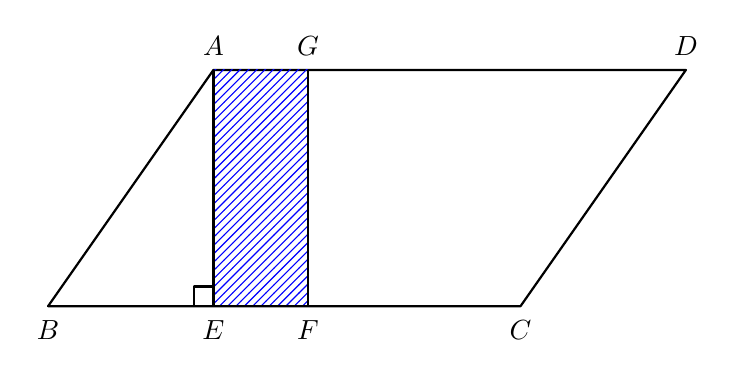
\begin{tikzpicture}[scale=1,line width=0.8pt,line join=round,>=stealth]
		 
			\def\b{3}  
			\def\t{1.2}  
			 
			\path 
			(0,0) coordinate (B)
			(0:2*\b) coordinate (C)
			(0:0.7*\b)coordinate(E)
			(E)++(90:\b)coordinate(A)
			(A)++(0:2*\b)coordinate(D)
			(E)++(0:\t)coordinate(F)
			(F)++(90:\b)coordinate(G)
			;
			
		 
			\draw (A)--(B)--(C)--(D)--cycle;
		 
			\fill[pattern=north east lines, pattern color=blue](A)--(E)--(F)--(G);
			 \draw   (A)--(E)--(F)--(G);
		  %%%% Hiển thị tên điểm
		 \foreach \x/\g in {A/90,B/-90, C/-90,D/90,E/-90,F/-90,G/90
		 }\draw[fill=white](\x)circle(0pt)+(\g:.3)node{$\x$};
		 \draw pic[draw, angle radius=2.5mm]{right angle=A--E--B};
		\end{tikzpicture}
	\end{center}
	
	\begin{listEX}
		\item Tính diện tích mảnh đất hình bình hành đó.
		\item Chủ mảnh đất làm một lối đi hình chữ nhật $AEFG$ có kích thước $AG = 12$ dm, $AE = 3$ m.  
		Hỏi diện tích mảnh đất hình bình hành gấp mấy lần diện tích lối đi hình chữ nhật?
		\item Để lối đi sạch đẹp hơn, chủ nhà lát những viên gạch hình vuông kín lối đi.  
		Hỏi chủ nhà sử dụng những viên gạch hình vuông có độ dài cạnh lớn nhất bằng bao nhiêu để không có viên gạch nào bị cắt xén (coi mạch vữa không đáng kể) và khi đó người chủ cần bao nhiêu viên gạch?
	\end{listEX}
	
	\loigiai{a) $18$ m$^2$ \hfill b) $5$ (lần) \hfill c) $10$ (viên)
	}
\end{bt}


%%%%%%%%%%%%%%% BÀI 6
\begin{bt}%[Thống kê huy chương theo điểm]
	Trong một kỳ thi quốc tế, các thành viên của đội tuyển Việt Nam đạt được số điểm lần lượt là:
	$26;  18; 36;  28;  21; 32.$
	Biết rằng người ta phân loại huy chương theo điểm số như sau:
	 \begin{center}
	\begin{tabular}{|c|c|}
		\hline
		\textbf{Khoảng điểm} & \textbf{Loại huy chương} \\ \hline
		Từ $15$ đến dưới $24$ & Huy chương đồng \\ \hline
		Từ $24$ đến dưới $31$ & Huy chương bạc \\ \hline
		Từ $31$ trở lên & Huy chương vàng \\ \hline
	\end{tabular}
	\end{center}
	Hãy lập bảng thống kê số lượng huy chương đồng, bạc, vàng mà đội tuyển Việt Nam đạt được trong kỳ thi này.
	\loigiai{
		\\
		\begin{tabular}{|c|c|}
			\hline
			\textbf{Loại huy chương} & \textbf{Số lượng} \\ \hline
			Đồng & $2$ \\ \hline
			Bạc & $2$ \\ \hline
			Vàng & $2$ \\ \hline
		\end{tabular}
	}
\end{bt}


%%%%%%%%%%%%%%% BÀI 7
\begin{bt} 
	Tìm $x, y$ biết: $\overline{1xy}$ là bội của $9$ và $x$ là số nguyên tố lẻ nhỏ nhất.
	\loigiai{ $135$}
\end{bt}  
\Closesolutionfile{ansbook} 
\newpage

%%%%%%%%%%%%%% ĐỀ SỐ 24
\Opensolutionfile{ansbook}[ans/ansD24] 	
\section{ĐỀ SỐ \thesection } %star8
\setcounter{bt}{0}

\begin{bt}
	 Thực hiện phép tính (tính hợp lý nếu có thể): 
	\begin{listEX}[2]
		\item $3\cdot 6+63:3^2$;
		\item $67\cdot 42+67\cdot 58-700$;
		\item $2025^{2025}:2025^{2024}+\bigl[1080-\bigl(3\cdot 3^3+999\bigr)\bigr]$.
	\end{listEX}
	\loigiai{a) $25$ \hfill b) $6000$ \hfill c) $2025$}
\end{bt}

\begin{bt}
	 Tìm số nguyên $x$ biết:
	\begin{listEX}[2]
		\item $1200:(x-10)=400-3\cdot 10^2$;
		\item $4^x\cdot 4^{2x+1}=16^5$;
		\item $2^{x+2}-6=4^2-(2^3-2)$;
		\item $20-3|x-4|=8$.
	\end{listEX}
	\loigiai{a) $22$ \hfill b) $3$ \hfill c) $2$ \hfill d) $x=0$ hoặc $x=8$}
\end{bt}

\begin{bt}
	Chị Hoa có một số bông sen. Nếu chị bó thành các bó gồm $5$ bông, $8$ bông, $10$ bông thì đều vừa hết. Hỏi chị Hoa có bao nhiêu bông sen? Biết rằng chị Hoa có khoảng từ $100$ đến $150$ bông sen.
	\loigiai{$120$ bông sen.}
\end{bt}

\begin{bt}
	
	Cô Ngọc muốn chia $160$ quyển vở, $96$ chiếc bút chì và $192$ chiếc bút bi thành một số phần thưởng như nhau để trao trong dịp tổng kết học kì I. Hỏi cô Ngọc có thể chia thành nhiều nhất bao nhiêu phần thưởng? Khi chia được số phần thưởng nhiều nhất thì mỗi phần thưởng có bao nhiêu quyển vở, bao nhiêu bút chì và bao nhiêu bút bi?
	\loigiai{$32$ phần thưởng. Khi đó:
		số vở mỗi phần $5$, số bút chì mỗi phần $3$,số bút bi mỗi phần $6$. }
\end{bt}

\begin{bt}
	 Tìm $x$ biết $x \vdots 10$, $x \vdots 16$, $x \vdots 32$ và $200<x<380$.
	\loigiai{  $x=320$. }
\end{bt}

\begin{bt}
	Một ngôi nhà có bãi cỏ bao quanh như hình bên.
	
	\begin{center}
		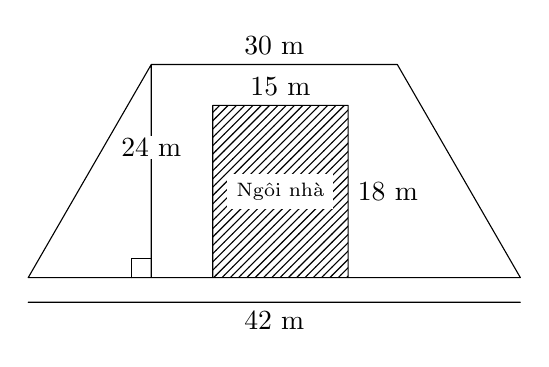
\begin{tikzpicture}[scale=1.25,line join=round,line cap=round,>=stealth]
			\def\a{2.5} 
			
			\path
			(0,0)coordinate(D)
			(0:2*\a)coordinate(C)
			(60:\a)coordinate(A)
			(C)++(120:\a)coordinate(B)
			($(D)!(A)!(C)$) coordinate(H)
			(H)++(0:0.25*\a)coordinate(E)
			(E)++(0:0.55*\a)coordinate(F)
			(E)++(90:0.7 *\a)coordinate(R)
			(F)++(90:0.7 *\a)coordinate(X)
			
			(D)++(-90:0.1*\a)coordinate(x)
			(C)++(-90:0.1*\a)coordinate(y)
			;
			\draw 
			(A)--(B)node[midway,above]{30 m}--(C)--(D)--(A)--(H)node[midway,shift={(90:0.3)},fill=white,inner sep=1pt,rectangle]{ 24 m} (E)--(R)--(X)node[midway,above]{15 m}--(F)node[midway,right]{18 m}
			(x)--(y)node[midway,below]{42 m}
			; 
			\fill[pattern = north east lines, pattern color=black] (R)--(X)--(F)--(E)--(R);
			
				\path ($(R)!0.5!(F)$) node[fill=white](c) {\scriptsize Ngôi nhà};
			
			%%%% Hiển thị tên điểm
		%	\foreach \x/\g in {C/-90,B/90,A/90,D/-90,H/-90,E/45,F/45,R/180,X/9}\draw[fill=white](\x)circle(1.5pt)+(\g:.3)node{$\x$};
			
			\foreach \x/\y/\z in {A/H/D}{
				\path pic[draw,angle radius=7pt]{right angle= \x--\y--\z};
			}
		\end{tikzpicture}\\
	\end{center}
	
	\begin{listEX}
		\item Hãy tính diện tích của bãi cỏ.
		\item Nếu một túi hạt giống cỏ gieo vừa đủ trên $54$ m$^2$ đất, thì cần bao nhiêu túi hạt giống để gieo vừa hết bãi cỏ?
	\end{listEX}
	
	\loigiai{a) $594$ m$^2$ \hfill b) $11$ túi hạt giống.}
\end{bt}


\begin{bt}
	\text{ }
	\begin{listEX} 
		 \item Biểu đồ tranh dưới đây biểu diễn số cây của các lớp khối $6$ trồng được trong ngày hội trồng cây (mỗi \faTree\ ứng với $5$ cây). Hỏi lớp nào trồng được nhiều cây nhất và trồng được bao nhiêu cây? \begin{center}
		 	
			\begin{tabular}{|c|c|}\hline
				Lớp $6$A & \faTree\ \faTree\ \faTree\\\hline
				Lớp $6$B & \faTree\ \faTree\ \faTree\ \faTree\\\hline
				Lớp $6$C & \faTree\ \faTree\\\hline
				Lớp $6$D & \faTree\ \faTree\ \faTree\\\hline
			\end{tabular} 
		\end{center}
		\item  Điểm kiểm tra môn Toán của $44$ học sinh lớp $6$ được thống kê như sau. Hãy cho biết có bao nhiêu bạn đạt từ điểm $5$ trở lên?
		\begin{center}
			\begin{tabular}{|c|c|c|c|c|c|c|c|c|}\hline
				Điểm & $3$ & $4$ & $5$ & $6$ & $7$ & $8$ & $9$ & $10$\\\hline
				Số bạn & $4$ & $6$ & $9$ & $7$ & $7$ & $5$ & $4$ & $2$\\\hline
			\end{tabular}
		\end{center}
		\item  Bảng thống kê dưới đây ghi lại diện tích rừng nước ta bị chặt phá từ năm $1995$ đến năm $1998$. Tính tổng diện tích rừng bị chặt phá trong suốt $4$ năm?
		\begin{center}
			\begin{tabular}{|c|c|c|c|c|}\hline
				Năm & $1995$ & $1996$ & $1997$ & $1998$\\\hline
				Diện tích rừng (nghìn ha) & $20$ & $5$ & $8$ & $10$\\\hline
			\end{tabular}
		\end{center}
	\end{listEX}
	\loigiai{a) $20$ cây \hfill b) $34$ học sinh \hfill c) $43$ nghìn ha}
\end{bt}

\begin{bt}
	 Cho $A=3^1+3^2+3^3+\cdots+3^{2024}$. Chứng minh rằng $A$ chia hết cho $120$.
	\loigiai{
		Nhóm theo từng $4$ số hạng:
		\[
		A=\underbrace{(3^1+3^2+3^3+3^4)}_{=120}
		+3^4\underbrace{(3^1+3^2+3^3+3^4)}_{=120}
		+\cdots
		+3^{2020}\underbrace{(3^1+3^2+3^3+3^4)}_{=120}.
		\]
		Do $3^1+3^2+3^3+3^4=3+9+27+81=120$, suy ra $A=120\bigl(1+3^4+3^8+\cdots+3^{2020}\bigr)$, nên $A$ chia hết cho $120$.
	}
\end{bt}
 
\Closesolutionfile{ansbook} 
\newpage

%%%%%%%%%%%%%% ĐỀ SỐ 25
\Opensolutionfile{ansbook}[ans/ansD25] 	
\section{ĐỀ SỐ \thesection} %star10
\setcounter{bt}{0}

%%%%%%%%%%%%%%% CÂU 1
\begin{bt}  Tính hợp lý (nếu có thể)
	\begin{listEX}[2]
		\item  $(-67)+125+(-33)+75$;
		\item $600- \dfrac{36+4^3}{5^2} $;
		\item $(-3023)-\left(765-3023\right)$;
		\item $798-\dfrac{298}{\,19-2\cdot\left(5^2-22^2\right)}\cdot 1^{2024}$.
	\end{listEX}
	\loigiai{a) $100$ \hfill b) $596$ \hfill c) $-765$ \hfill d) $\dfrac{747428}{937}\approx 797{,}682$
	}
\end{bt}

%%%%%%%%%%%%%%% BÀI 2
\begin{bt}  Tìm $x\in \mathbb{Z}$
	\begin{listEX}[2]
		\item  $71-\left(24-3\cdot x\right)=23$;
		\item $3^{x-1}+5\cdot 3^x=432$;
		\item $2x+(-2)\cdot\left|5-x\right|-|-4|=-18+2x$;
		\item $\left(x^2+9\right)\cdot\left(x-2\right)=0$.
	\end{listEX}
	\loigiai{ a)$x=-8$ \hspace{1cm}
			b) $x=4$\hspace{1cm}
			c) $x=12$ hoặc $x=-2$\hspace{1cm}
			d) $x=2$ 	}
\end{bt}

%%%%%%%%%%%%%%% BÀI 3
\begin{bt} 
	Star Education tổ chức cho các bạn học sinh đạt thành tích cao trong bài kiểm tra cuối khóa đi tham quan bằng ô tô. Khi xếp lên các xe $36$ chỗ ngồi, xe $40$ chỗ ngồi hay xe $45$ chỗ ngồi thì các xe đều vừa đủ chỗ. Tính số học sinh đi tham quan của trung tâm? Biết rằng số học sinh đó khoảng $1000$ đến $1100$ học sinh. Nếu cả trung tâm cùng đi xe $45$ chỗ ngồi thì cần bao nhiêu xe để xếp đủ học sinh?
	\loigiai{
		Số xe $45$ chỗ cần dùng là $24$ xe
	}
\end{bt}

%%%%%%%%%%%%%%% BÀI 4
\begin{bt} 
	Một người đi xe đạp từ $B$ đến $C$ với vận tốc $15$ km/giờ, cùng lúc đó một người đi xe máy từ $A$ cách $B$ $50$ km với vận tốc $40$ km/giờ và đuổi theo người đi xe đạp. Kể từ lúc bắt đầu sau mấy giờ xe máy đuổi kịp xe đạp?
	\loigiai{$2$ giờ.
	}
\end{bt}

%%%%%%%%%%%%%%% BÀI 5
\begin{bt} 
	Một mảnh đất hình chữ nhật có chiều dài $40$ m, chiều rộng $25$ m.
	Người ta làm một sân khấu hình thang cân có kích thước như hình bên dưới.
	
	\immini{\begin{listEX}
		\item Tính diện tích mảnh đất và sân khấu.
		\item Trang trí sân khấu người ta phải trả cho mỗi mét vuông sân khấu là $500\,000$ đồng/m$^2$. Hỏi người ta phải chi hết bao nhiêu tiền để trang trí sân khấu?
	\end{listEX}}{ 
	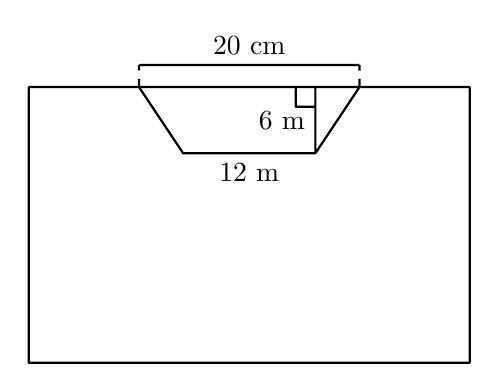
\begin{tikzpicture}[scale=0.14,line width=0.8pt,line join=round,>=stealth]
		
		\def\a{6}  
		\def\b{5} 
		\def\c{4} 
		
		\path 
		(0,0) coordinate (B)
		(0:8*\b) coordinate (C)
		(90:5*\b)coordinate(A)
		(A)++(0:8*\b) coordinate (D) 
		(A)++(0:2*\b) coordinate (E) 
		(E)++(0:4*\b) coordinate (F)
		(E)++(0: \c) coordinate (G) 
		(F)++(0: -\c) coordinate (H)
		(G)++(90: -\a) coordinate (G') 
		(H)++(90: -\a) coordinate (H')
		
		(E)++(90:0.5*\c) coordinate (E') 
		(F)++(90:0.5*\c) coordinate (F')
		;
		
		
		\draw (A)--(B)--(C)--(D)--cycle
		(E)--(G')--(H')node[midway,below]{12 m}--(F) (H')--(H)node[midway,left]{6 m}
		
		(E')--(F')node[midway,above]{20 cm}
		;
		\draw[dashed](E)--(E') (F)--(F')
		;
		
		%%%% Hiển thị tên điểm
		%	\foreach \x/\g in {A/90,B/-90, C/-90,D/90,E'/9,F'/9 ,E/90,F/90,G/9,H/9,G'/9,H'/9
			%	}\draw[fill=white](\x)circle(1.5pt)+(\g:.3)node{$\x$};
		
		\draw pic[draw, angle radius=2.5mm]{right angle=E--H--H'};
	\end{tikzpicture}
 }
	
	
	
	
	\loigiai{a) $1\,000$ m$^2$, $96$ m$^2$ \hfill b) $48\,000\,000$ đồng.
	}
\end{bt}

%%%%%%%%%%%%%%% BÀI 6
\begin{bt} 
	Kết quả điều tra về loại quả ưa thích nhất đối với một số bạn trong lớp, mỗi bạn trả lời một lần, được ghi lại trong bảng sau:
	$$
	\begin{array}{|c|c|c|c|c|}
		\hline
		\text{Cam} & \text{Ổi} & \text{Chuối} & \text{Xoài} & \text{Cam} \\ \hline
		\text{Khế} & \text{Cam} & \text{Ổi} & \text{Khế} & \text{Xoài} \\ \hline
		\text{Xoài} & \text{Ổi} & \text{Chuối} & \text{Xoài} & \text{Khế} \\ \hline
		\text{Xoài} & \text{Cam} & \text{Khế} & \text{Cam} & \text{Xoài} \\ \hline
		\text{Ổi} & \text{Khế} & \text{Xoài} & \text{Chuối} & \text{Cam} \\ \hline
	\end{array}
	$$
	\begin{listEX}
		\item Có bao nhiêu bạn tham gia trả lời?
		\item Hãy lập bảng thống kê và cho biết loại quả nào được các bạn yêu thích nhất.  
	\end{listEX}
	\loigiai{
		\begin{listEX}
			\item Có $25$ bạn tham gia trả lời.
			\item Bảng thống kê:
		\end{listEX}
		$$
		\begin{array}{|c|c|c|c|c|c|}
			\hline
			\textbf{Quả yêu thích} & \text{Cam} & \text{Ổi} & \text{Chuối} & \text{Khế} & \text{Xoài} \\ \hline
			\textbf{Số bạn chọn} & 6 & 4 & 3 & 5 & 7 \\ \hline
		\end{array}
		$$
		Vậy Xoài được các bạn yêu thích nhất.
	}
\end{bt}

%%%%%%%%%%%%%%% BÀI 7
\begin{bt} 
	Hãy tính
	$$
	A=2+2^2+2^3+2^4+\ldots+2^{100}.
	$$
	\loigiai{
		\begin{align*}
			A&=2+2^2+2^3+\ldots+2^{100}\\
			2A&=2\cdot 2+2^2\cdot 2+\ldots+2^{100}\cdot 2=2^2+2^3+\ldots+2^{101}\\
			2A-A&=\left(2^2+2^3+\ldots+2^{101}\right)-\left(2+2^2+\ldots+2^{100}\right)\\
			\text{Vậy} A&=2^{101}-2.
		\end{align*}
	}
\end{bt}
  
\Closesolutionfile{ansbook} 
\newpage
         %------------------------%
\part{TRẮC NGHIỆM}
 	\setcounter{section}{0}
	\setcounter{section}{0}
%%%%%%%%%%%%%% PHẦN ĐẠI SỐ
		\Opensolutionfile{ans}[ans/TN-DS] 
		
\section{ĐẠI SỐ}
\setcounter{ex}{0}
%1
\begin{ex}
	Trong các tập hợp sau, tập hợp nào có các phần tử đều là số nguyên tố? 
	\choice
	{$\{1;3;5;7;19\}$}
	{$\{2;3;5;7;9\}$}
	{\True $\{2;3;5;7;11\}$}
	{$\{0;3;5;7;13\}$}		
\end{ex}
%2
\begin{ex} Tập hợp $A = \{0; 1; 2; 3; 4; 5; 6; 7; 8; 9; 10\}$. Phát biểu nào sau đây là đúng?
	\choice
	{$11 \in A$}
	{$1 \notin A$}
	{\True $10 \in A$}
	{$7 \notin A$}
\end{ex}
%3
\begin{ex}
	Trong một hội nghị có 100 đại biểu tham dự. Mỗi đại biểu nói được một hoặc hai hoặc ba \\
	\begin{minipage}{0.6\textwidth}
	 thứ tiếng: Nga, Anh hoặc Pháp. Biết rằng có 39 đại biểu chỉ nói được tiếng Anh, 35 đại biểu nói được tiếng Pháp, 8 đại biểu nói được cả tiếng Anh và tiếng Nga. Hỏi có bao nhiêu đại biểu chỉ nói được tiếng Nga?
	
	
		\hfill
		\choice
		{$26$ đại biểu}
		{$53$ đại biểu}
		{\True $18$ đại biểu}
		{$20$ đại biểu}
	\end{minipage}
	\begin{minipage}{0.4\textwidth}
		
			%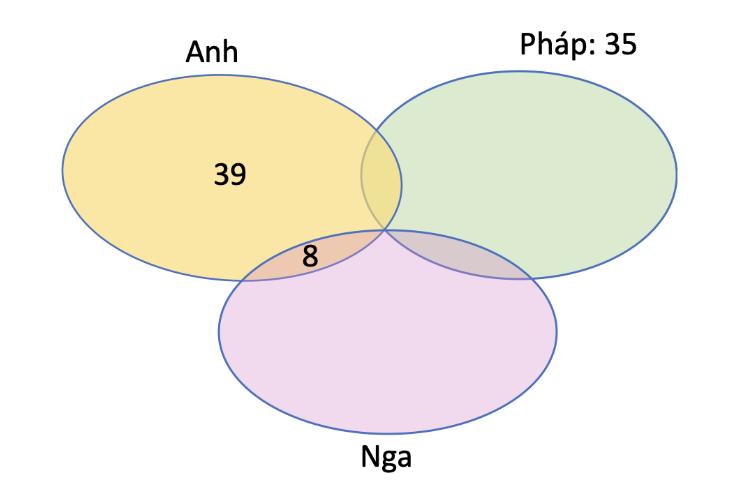
\includegraphics[scale=0.3]{data/Hình/H2}\\
		
		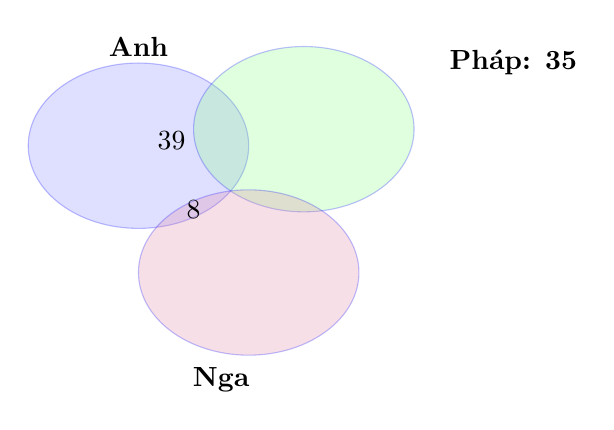
\begin{tikzpicture}[scale=0.7]
			
			%--- Ellipse Anh ---
			\fill[blue!50, opacity=0.25, draw=blue]
			(-1.5,0) ellipse (2 and 1.5);
			
			%--- Ellipse Pháp ---
			\fill[green!50, opacity=0.25, draw=blue]
			(1.5,0.3) ellipse (2 and 1.5);
			
			%--- Ellipse Nga ---
			\fill[purple!50, opacity=0.25, draw=blue]
			(0.5,-2.3) ellipse (2 and 1.5);
			
			%--- Labels ---
			\node at (-1.5,1.8) {\bf Anh};
			\node at (5.3,1.5) {\bf Pháp: 35};
			\node at (0,-4.25) {\bf Nga};
			
			%--- Numbers ---
			\node at (-0.9,0.1) {39};
			\node at (-0.5,-1.15) {8};
			
		\end{tikzpicture}
		
	\end{minipage}%
\end{ex}
%4
	\begin{ex} % Câu 1%[6D1B5-6]%[Dự án đề kiểm tra Toán 6 HKI NH23-24-NGUYỄN VĂN HỮU]%[THCS TÂN TRÀO]
	Kết quả phép tính $3^{2023}$ $:$ $3^{2020}$ là
	\choice
	{$3^{4}$}
	{$27$}
	{$3^{3}$}
	{\True Cả B, C đều đúng}
\end{ex}
%5
\begin{ex}%[6D1Y8-1]%[Dự án đề kiểm tra Toán 7 HKI NH23-24- Nguyễn Văn Hiệp]%[THCS Qui Đức]
	Số nào sau đây chia hết cho cả $2$, $3$	và $5$ nhưng không chia hết cho $9$?
	\choice
	{\True $240$}
	{$270$}
	{$235$}
	{$532$}
\end{ex}
%6
\begin{ex}%%câu 1
	Khẳng định nào sau đây \textbf{sai}?
	\choice
	{Nếu $a\ \vdots\ 3$ và $b\ \vdots\ 3$ thì $(a+b)\ \vdots\ 3$}
	{Nếu $a\ \vdots\ 2$ và $b\ \vdots\ 2$ thì $(a-b)\ \vdots\ 2$}
	{Nếu $a\ \vdots\ 4$ và $b\not\vdots\ 4$ thì $(a+b)\not\vdots\ 4$}
	{\True Nếu $a\ \vdots\ 5$ và $b\ \vdots\ 4$ thì $(a+b)\ \vdots\ 20$}	
\end{ex}
%7
\begin{ex} Hợp số là gì: 
	\choice
	{Hợp số là số tự nhiên}
	{Hợp số là số tự nhiên khác 0 có hai ước}
	{Hợp số là số tự nhiên khác 0 có nhiều hơn hai ước}
	{\True Hợp số là số tự nhiên lớn hơn 1 và có nhiều hơn hai ước}
\end{ex}

\begin{ex}%[6D1BC-2]%[Dự án đề kiểm tra HKI NH23-24- Dương BùiĐức]
	ƯCLN($12; 36$) bằng
	\choice
	{$15$}
	{$30$}
	{$6$}
	{\True $12$}
\end{ex}

\begin{ex}%[6D1KD-3] %[Dự án đề kiểm tra Toán 6 HKI NH23-24-NGUYỄN VĂN HỮU]%[THCS TÂN TRÀO]
	Tìm tất cả Bội chung nhỏ hơn $ 100 $ của $ 7 $ và $ 6 $ ?
	\choice
	{\True $\{0 ; 42 ; 84\}$}
	{$\{42 ; 84\}$}
	{$\{84\}$}
	{$\{42\}$}
\end{ex}


\begin{ex}%[6D1KC-3] %[Dự án đề kiểm tra Toán 6 HKI NH23-24- Phạm Văn Long]%[THCS Bình Chánh]
	Lớp 6A có $21$ bạn nam và $27$ bạn nữ. Trong tiết Toán, thầy Lâm yêu cầu lớp trưởng tiến hành chia nhóm để các bạn hoạt động xây dựng bài học mới, sao cho số bạn nam và nữ trong mỗi nhóm bằng nhau. Số nhóm nhiều nhất trong lớp có thể chia được là:
	\choice
	{\True $3$}
	{$4$}
	{$5$}
	{$6$}
\end{ex}

\begin{ex} %[6D1TD-3]
	Bốn chiếc đồng hồ reo chuông tương ứng sau mỗi $5$ phút, $10$ phút, $15$ phút và $20$ phút. Chúng bắt đầu cùng reo chuông vào lúc $12$ giờ trưa. Lần tiếp theo chúng cùng reo chuông vào lúc nào?
	\choice
	{\True $13$ giờ trưa}
	{$13$ giờ $20$ trưa}
	{$12$ giờ $45$ trưa}
	{$12$ giờ $30$ trưa}
\end{ex}

\begin{ex}%[6D1KB-2]
	Một lớp có $42$ học sinh. Hỏi có bao nhiêu cách chia tổ, biết rằng số học sinh sau khi chia vào các tổ phải bằng nhau và số tổ lớn hơn $3$, nhỏ hơn $7$?
	\choice
	{\True Có $1$ cách chia tổ} 	
	{Có $6$ cách chia tổ}
	{Có $3$ cách chia tổ}	
	{Có $8$ cách chia tổ}
\end{ex}

\begin{ex}
	Số nào sau đây là số nguyên?
	\choice
	{$-0{,}8$}
	{\True $-8$}
	{$3{,}2$}
	{$\dfrac{-5}{2}$}
\end{ex}

\begin{ex} %C11
	Trong các tập hợp sau, tập hợp nào có các phần tử được xếp theo thứ tự tăng dần:
	\choice
	{$\{2;-17;5;1;-2;0\}$}
	{$\{-2;-17;0;1;2;5\}$}
	{\True $\{-17;-2;0;1;2;5\}$}
	{$\{0;1;2;5;-17\}$}
\end{ex}

\begin{ex}%[6D2B2-2]
	Các vị trí $a$, $b$, $c$ ở hình sau đây biểu diễn các số nguyên nào?
	\begin{center}
		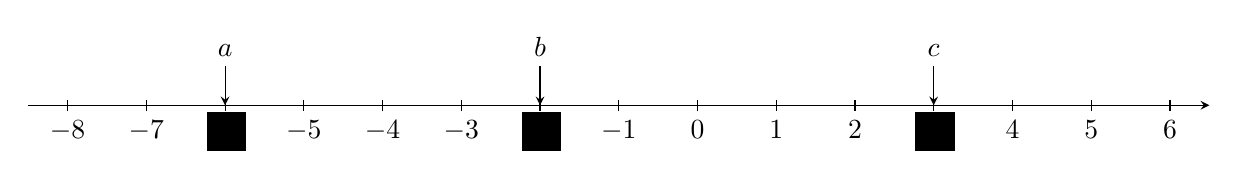
\begin{tikzpicture}[>=stealth]
			\draw[->] (-8.5,0)--(6.5,0);
			\foreach \x in {-8,...,6}
			\draw[shift={(\x,0)}] (0,2pt)--(0,-2pt) node[below]{ $\x$};
			\foreach \x/\y in {-6/a,-2/b,3/c}{
				\draw[<-] (\x,0)--++(90:.5)node[above]{$\y$};
				\fill ([shift={(200:.25)}]\x,0) rectangle ++(.5,-.5);
			}
			
		\end{tikzpicture}
	\end{center}
	\choice
	{\True $-6$; $-2$ và $3$}
	{$3$; $-2$ và $-6$}
	{$2$ và $6$}
	{$-2$ và $-6$}
	
\end{ex}

\begin{ex}%C8
	Số đối của $-(-a)$ là
	\choice
	{\True $-a$}
	{$a$}
	{$0$}
	{$1$}
\end{ex}

\begin{ex}%[6D2B4-1]%[Dự án đề kiểm tra HKI NH23-24- Dương BùiĐức]
	Kết quả phép tính $-268+47-32+53$ là
	\choice
	{\True $- 200$}
	{$200$}
	{$336$}
	{$-336$}
\end{ex}

\begin{ex}  %[6D1Y4-1]
	Kết quả của phép tính $(50-20):(-2)+1$ là
	\choice
	{\True $-14$}
	{$14$}
	{$16$}
	{$-16$}
\end{ex}

\begin{ex}%C9
	Nhận định nào sau đây đúng?
	\choice
	{$(-4) \cdot 8>0$}
	{$(-4) .(-8)<0$}
	{\True $4 .(-8)<0$}
	{$(-4) \cdot(-8)=-32$}
\end{ex}


\begin{ex}
	Tính tổng tất cả số nguyên $x$ thỏa $-3<x<3$ là
	\choice
	{$-3$}
	{$3$}
	{$6$}
	{\True $0$}
\end{ex}

\begin{ex} Tìm số nguyên $x$, thỏa mãn: $x^2=81$
	\choice
	{$x=9$}
	{$x=-9$}
	{\True $x=9$ hoặc $x=-9$}
	{$x=3$}
\end{ex}	
%22
\begin{ex}
	Tập hợp các ước nguyên của $9$ là	
	\choice
	{Ư$(9) = \{0; 1; -1; 3; -3; 9; -9\}$}
	{Ư$(9) = \{ 1; -1; 3; -3; 6; 9\}$}
	{\True Ư$(9) = \{ 1; -1; 3; -3; 9; -9\}$}
	{Ư$(9) = \{1; 3; 6; 9\}$}	
\end{ex}

\begin{ex}
	Lợi nhuận của công ty An Bình trong $4$ tháng đầu năm là $-40$ triệu đồng mỗi tháng. Lợi nhuận trong $8$ tháng sau đó là $80$ triệu mỗi tháng. Hỏi sau $1$ năm công ty An Bình có lợi nhuận là bao nhiêu triệu đồng?
	\choice
	{$120$} 
	{\True $480$}
	{$40$} 
	{$420$}
\end{ex}

%Câu 3
\begin{ex}
	Một tàu ngầm đang ở độ sâu $20$ m, nếu tàu ngầm tiếp tục lặn xuống thêm $15$ m nữa, khi đó tàu ngầm ở độ cao so với mực nước biển là
	\choice
	{\True $-35$ m}
	{$-5$ m}
	{$15$ m}
	{$35$ m}
\end{ex}

%%%============CÂU 25 ==============%%%

\begin{ex} %[6D2T4-1]
	Ban ngày, nhiệt độ ở New York (Niu Oóc) là $-5^{\circ} {C}$. Nhiệt độ ban đêm là $-14^{\circ} {C}$. Tính chênh lệch nhiệt độ giữa ngày và đêm ở New York?
	\choice
	{$-19^{\circ} {C}$}
	{$-9^{\circ} {C}$}
	{\True $9^{\circ} {C}$}
	{$19^{\circ} {C}$}
\end{ex}




  
		\Closesolutionfile{ans}
%%%%%%%%%%%%%% PHẦN HÌNH HỌC
		\Opensolutionfile{ans}[ans/TN-HH] 
		\section{HÌNH HỌC}
\setcounter{ex}{0}


%%Câu 1          
\begin{ex}
	Chọn theo đúng thứ tự xuất hiện của hình $1$, hình $2$, hình $3$.
	\begin{center}
		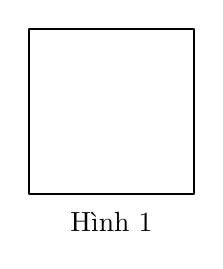
\begin{tikzpicture}[scale=.7,line width=0.8pt, line join=round, line cap=round,>=stealth]
			\draw
			(0,0)rectangle (3,3)
			(1.5,-0.5)node{Hình $1$}
			;
		\end{tikzpicture}\hspace*{1cm}
		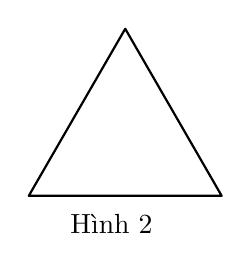
\begin{tikzpicture}[scale=.7,line width=0.8pt, line join=round, line cap=round,>=stealth]
			\draw
			(0,0)--+(0:3.5)--+(60:3.5)--cycle
			(1.5,-0.5)node{Hình $2$}
			;
		\end{tikzpicture}\hspace*{1cm}
		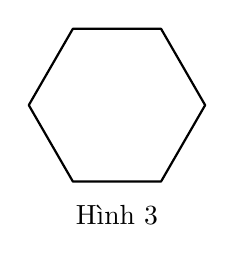
\begin{tikzpicture}[scale=.7,line width=0.8pt, line join=round, line cap=round,>=stealth]
			\path
			(0,0)+(0:1.6)coordinate(A)
			+(60:1.6)coordinate(B)
			+(120:1.6)coordinate(C)
			+(180:1.6)coordinate(D)
			+(240:1.6)coordinate(E)
			+(300:1.6)coordinate(F)
			
			;
			\draw
			(A)--(B)--(C)--(D)--(E)--(F)--cycle
			(0,-2)node{Hình $3$}
			;
		\end{tikzpicture}
	\end{center}
	\choice
	{Tam giác đều – Hình vuông – Lục giác đều}
	{\True Hình vuông – Tam giác đều – Lục giác đều}
	{Hình chữ nhật – Tam giác đều  - Lục giác đều}
	{Hình vuông – Tam giác cân – Lục giác đều}
\end{ex}

%%Câu 5
\begin{ex}%[6H1Y1-1]%[Dự án đề kiểm tra HKI NH23-24- Dương BùiĐức]
	Trong các hình sau đây, hình nào là tam giác đều?
	\begin{center}
		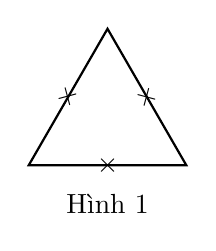
\begin{tikzpicture}[line width=0.8pt,scale=0.8]
			\def\h{2.5}
			\def\goc{60}
			\path
			(0,0) coordinate (B)
			+(\goc:2*\h) coordinate (b)
			++(0:\h) coordinate (C)
			+(180-\goc:\h) coordinate (c)
			($(B)!1/2!(C)$) coordinate (H)
			(intersection of B--b and C--c) coordinate (A)
			;
			\pgfresetboundingbox
			\draw 
			(A)--(B)--(C)--cycle
			;
			\foreach \x/\y/\z in {
				C/B/\times,
				A/B/\times,
				A/C/\times
			}\path (\x)--(\y) node[pos=0.5,sloped]{$\z$};
			\path (current bounding box.south) node[below]{Hình 1};
		\end{tikzpicture} \hfil
		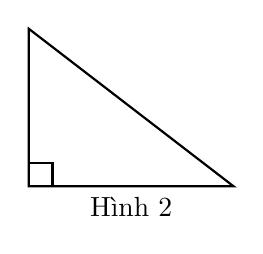
\begin{tikzpicture}[line width=0.8pt,scale=0.8]
			\def\h{2.5}
			\def\goc{90}
			\path
			(0,0) coordinate (B)
			+(\goc:\h) coordinate (A)
			++(0:1.3*\h) coordinate (C)
			;
			\pgfresetboundingbox
			\draw 
			(A)--(B)--(C)--cycle
			;
			
			\foreach \a/\b/\c in
			{A/B/C}{\draw pic[draw,angle radius=3mm] {right angle = \a--\b--\c};}
			\path (current bounding box.south) node[below]{Hình 2};
		\end{tikzpicture} \hfil
		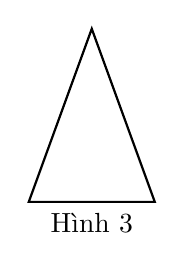
\begin{tikzpicture}[line width=0.8pt,scale=0.8]
			\def\h{2}
			\def\goc{70}
			\path
			(0,0) coordinate (B)
			+(\goc:2*\h) coordinate (b)
			++(0:\h) coordinate (C)
			+(180-\goc:\h) coordinate (c)
			($(B)!1/2!(C)$) coordinate (H)
			(intersection of B--b and C--c) coordinate (A)
			;
			\pgfresetboundingbox
			\draw 
			(A)--(B)--(C)--cycle
			;
			\path (current bounding box.south) node[below]{Hình 3};
		\end{tikzpicture} \hfil
		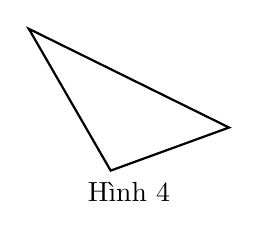
\begin{tikzpicture}[line width=0.8pt,scale=0.8]
			\def\h{2}
			\def\goc{70}
			\path
			(0,0) coordinate (B)
			+(20:\h) coordinate (C)
			+(120:1.3*\h) coordinate (A)
			;
			\pgfresetboundingbox
			\draw 
			(A)--(B)--(C)--cycle
			;
			\path (current bounding box.south) node[below]{Hình 4};
		\end{tikzpicture}
	\end{center}
	\choice
	{\True Hình 1}
	{Hình 2}
	{Hình 3}
	{Hình 4}
\end{ex}

\begin{ex}%[6H1Y1-1] 
	\immini{
		Tam giác ABC được gọi là tam giác đều nếu
		\choice
		{Mỗi góc đỉnh $A, B, C$ có số đo bằng $90^\circ$}
		{Mỗi góc đỉnh $A, B, C$ có số đo bằng $80^\circ$}
		{\True Mỗi góc đỉnh $A, B, C$ có số đo bằng $60^\circ$}
		{Mỗi góc đỉnh $A, B, C$ có số đo bằng $30^\circ$}
	}{
		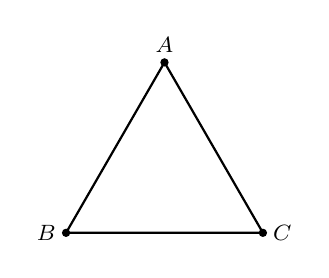
\begin{tikzpicture}[line join = round, line cap = round,line width=0.8pt,>=stealth,font=\footnotesize,scale=1] 
			\def\a{2.5}
			\def\goc{60}
			\coordinate[label = left:$B$] (B) at (0,0); 
			\coordinate[label = right:$C$] (C) at ($(B)+(\a,0)$); 
			\coordinate[label = above:$A$] (A) at ($(B)+(\goc:\a)$); 
			\draw (A)--(B)--(C)--cycle; 
			\foreach \x in {A,B,C} \fill[black] (\x) circle (1.5pt);
		\end{tikzpicture}
	}
\end{ex}

\begin{ex}%[6H1B4-1]
	Hình thang cân có các tính chất nào sau đây? 
	\choice
	{Có hai đường chéo vuông góc}
	{Có bốn cạnh bằng nhau}	
	{Có bốn cạnh song song với nhau}
	{\True Có hai góc kề một đáy bằng nhau}
\end{ex}

%%Câu 2
\begin{ex} 
	Yếu tố nào sau đây không phải của hình bình hành?
	\choice
	{ Hai cặp cạnh đối diện song song}
	{Hai cặp cạnh đối diện bằng nhau}
	{\True Hai đường chéo bằng nhau}
	{Hai đường chéo cắt nhau tại trung điểm của mỗi đường}
\end{ex}     

%%Câu 6
\begin{ex}
	Hình thoi là
	\choice
	{\True Hình có bốn cạnh bằng nhau}
	{Hình có bốn cạnh bằng nhau và bốn góc vuông}
	{Hình có hai đường chéo bằng nhau}
	{Hình có bốn góc bằng nhau và bằng góc vuông}
\end{ex}

%%Câu 9
\begin{ex}
	Khẳng định nào sau đây là đúng? Trong hình chữ nhật:
	\choice
	{Hai đường chéo song song với nhau}
	{\True Bốn góc bằng nhau}
	{Hai đường chéo không bằng nhau}
	{Bốn góc không bằng nhau}
\end{ex}

\begin{ex} 
	Ba đường chéo chính của lục giác đều $A B C D E F$ là
	\choice
	{$A B$, $C D$, $A C$}
	{\True $A D$, $F C$, $E B$}
	{$AB$, $CD$, $EF$}
	{$F E$, $E D$, $D C$}	
\end{ex}


%%% câu 7
\begin{ex}%[6H1Y1-1] 
	\immini{
		Cho hình vuông MNPQ, khẳng định nào sau đây \textbf{đúng}?
			\choice
		{MN và MQ song song}
		{MN và MP song song}
		{MQ và PQ song song}
		{\True MN và PQ song song}
	}{
		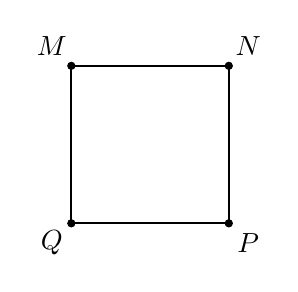
\begin{tikzpicture}[scale=1,line width=0.8pt,line join=round,>=stealth]
			\def\a{2} 
			\path (0,0) coordinate (M)
			(M)+(0:\a) coordinate (N)
			(N)+(-90:\a) coordinate (P)
			(M)+(-90:\a) coordinate (Q)
			;
			\draw (M)--(N)--(P)--(Q)--(M);
			\foreach \x/ \goc in {M/135,N/45,P/-45,Q/-135}  \fill (\x) circle (1.5pt) ($(\x)+(\goc:3.5mm)$) node {$\x$};
		\end{tikzpicture}
	}
\end{ex}

\begin{ex}%[6H1Y1-7] 
	Cho tam giác đều $ABC$ với $AB=17$ cm. Độ dài cạnh $BC$ là
	\choice
	{\True $17$ cm}
	{$7{,}5$ cm}
	{$30$ cm}
	{$5$ cm}
\end{ex}

%%Câu 10
\begin{ex} Hình thoi có độ dài hai đường chéo lần lượt là 15 cm, 20 cm thì diện tích hình thoi là:
	
	\choice
	{300}
	{\True 150}
	{70}
	{75}
\end{ex}

\begin{ex}
	Cho hình chữ nhật ABCD có AB= 3cm. Độ dài cạnh AD lớn hơn cạnh AB 4 cm. Chu vi hình chữ nhật ABCD là bao nhiêu cm.
	\choice
	{10}
	{\True 20}
	{21}
	{14}
	
\end{ex}

\begin{ex}\immini[thm]{
		Mỗi viên gạch hình vuông có cạnh $20$ cm. Tính chu vi hình vuông ghép bởi $4$ viên gạch hoa như hình vẽ dưới đây.
		\hfill
		\choice
		{$1600$ cm$^2$}
		{$1600$ cm}
		{$160$ cm$^2$}
		{\True $160$ cm}	
	}{
		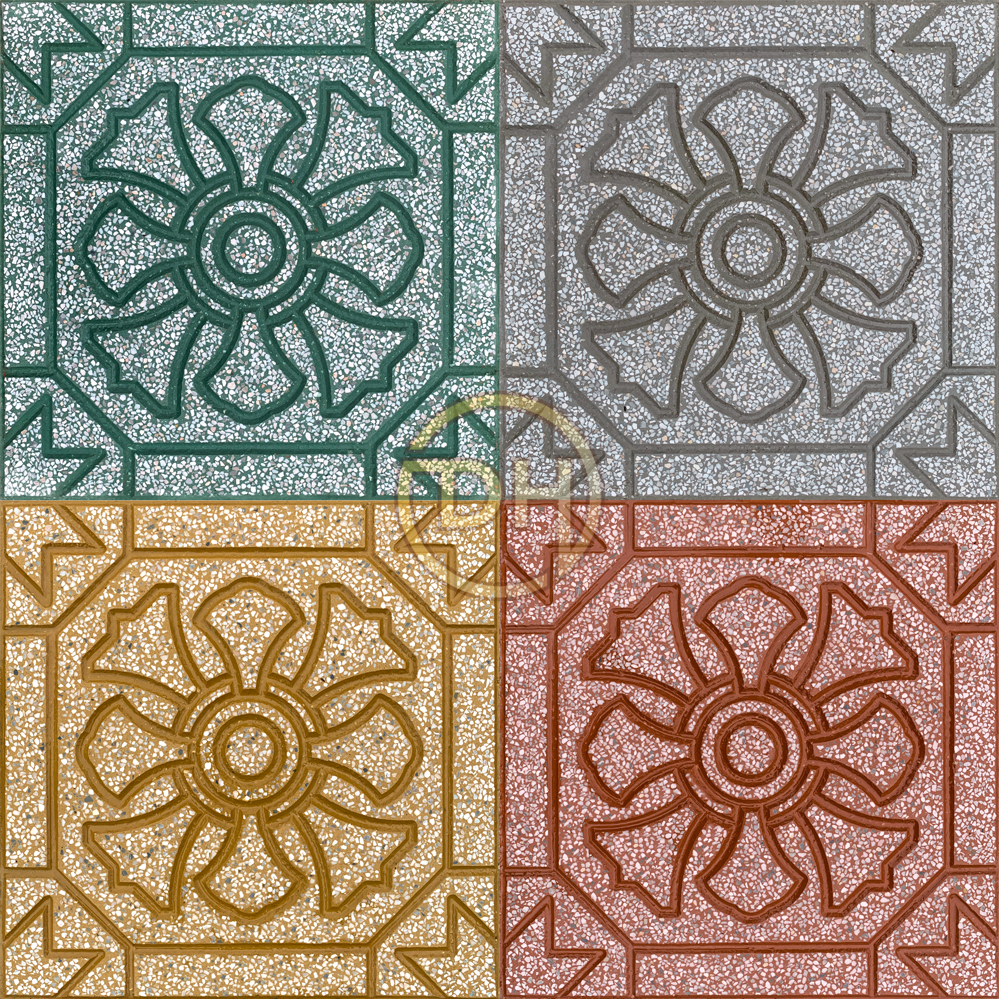
\includegraphics[scale=0.12]{data/Hình/C25_TN_HH}
	}
	
\end{ex}

\begin{ex}%Câu 8%[6H1Y1-4]% 
	Một hình vuông có diện tích $169 $ cm$^2$. Độ dài cạnh hình vuông là
	\choice
	{$10$ cm}
	{\True $13$ cm}
	{$36$  cm}
	{$24$ cm}
	
\end{ex}

%15
\begin{ex}%[6H1Y1-1] 
	\immini{
		 Khung của một bàn học làm bằng sắt được thiết kế như hình bên dưới. Mặt bàn là hình thang cân có đáy lớn dài $1200$ mm, đáy bé dài $600$ mm, cạnh bên dài $500$ mm. Mỗi chân bàn dài $730$ mm. Tính tổng độ dài các thanh sắt cần sử dụng để làm bàn học trên
		 	\choice
		 {\True $5720$ mm}
		 {$5220$ mm}
		 {$3030$ mm}
		 {$2530$ mm}
	}{
	%	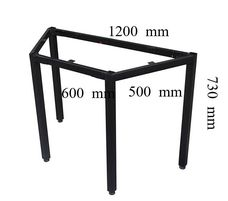
\includegraphics[width=4cm]{data/Hình/C6_HH_TN}
			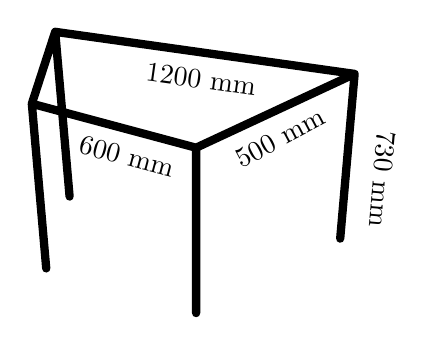
\begin{tikzpicture}[scale=1,line join=round,line cap=round,>=stealth]
			\def\a{1.2} 
			
			\path
			(0,0)coordinate(O)
			(-15:1.8*\a)coordinate(A)
			(72:0.8*\a)coordinate(D)
			(D)++(-8:3.2*\a)coordinate(C)
			(A)++(-90:1.75*\a)coordinate(A')
			(D)++(-85:1.75*\a)coordinate(D')
			(C)++(-95:1.75*\a)coordinate(C')
			(O)++(-85:1.75*\a)coordinate(O')
			($(O)!0.62!(A)$) node[below, rotate=-15,yshift=-0.1 cm]{$600$ mm}
			($(D)!0.5!(C)$) node[below, rotate=-8,yshift=-0.1 cm]{$1200$ mm}
			($(A)!0.45!(C)$) node[below, rotate=28,yshift=-0.1 cm]{$500$ mm}
			($(C)!0.62!(C')$) node[below, rotate=-95,yshift=0.7 cm]{$730$ mm}
			;
			\draw [line width=3pt]
			(O)--(A)-- (C)--(D)--(O)
			
			(A)--(A') (O)--(O') (C)--(C') (D)--(D')
			; 
			
			%%%% Hiển thị tên điểm
			%	\foreach \x/\g in {A/-40,D/90,C/90,O/-130
				%	}\draw[fill=white](\x)circle(1.5pt)+(\g:.3)node{$\x$};
		\end{tikzpicture}
	}
\end{ex}

%%Câu 18:
\begin{ex}
	\immini[thm]{
		Tính diện tích phần gạch sọc trong hình sau biết các kích thước như hình vẽ:
		\choice
		{$56$ m$^2$}
		{$42$ m$^2$}
		{$36$ m$^2$}
		{\True $28$ m$^2$}
	}{
	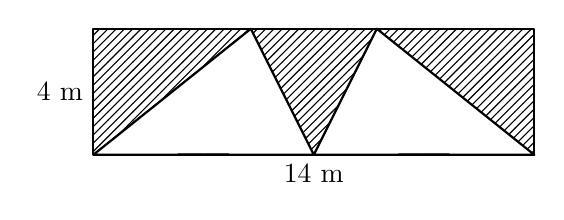
\begin{tikzpicture}[scale=1,line width=0.8pt,line join=round,>=stealth]
		\def\sc{2.5} 
		\path (0,0) coordinate (A)
		(A)+(0:14/\sc) coordinate (B)
		(B)+(-90:4/\sc) coordinate (C)
		(C)+(180:14/\sc) coordinate (D)
		(C)+(180:7/\sc) coordinate (G)node[below]{14 m}
		(A)+(0:5/\sc) coordinate (E)
		(A)+(0:9/\sc) coordinate (F)
		;
		\filldraw[pattern=north east lines] (D)--(A)node[midway,left]{4 m}--(B)--(C)--(G)--(D);
		\draw[fill=white] (D)--(E)--(G)--(F)--(C)--cycle;
		\draw (C)--(G)node[midway]{\small ||}--(D)node[midway]{\small ||};
	\end{tikzpicture}	
	}

\end{ex}



%%=====Câu 46
\begin{ex}%[6H1B2-4] 
	Một hình thoi có diện tích bằng $24$ cm$^2$. Biết độ dài một cạnh đường chéo bằng $6$ cm, tính độ dài đường chéo còn lại của hình thoi đó.
	\choice
	{$4$ cm}
	{$16$ cm}
	{$12$ cm}
	{\True $8$ cm}
\end{ex}


%%=====Câu 48
\begin{ex}\immini[thm]{
	Tính diện tích và chu vi phần in đậm trong hình dưới dây gần nhất với kết quả nào?
	\choice
	{16,8 cm$^2$; 14,9 cm$^2$}
	{7,4 cm$^2$; 14,9 cm$^2$}
	{\True 16,8 cm$^2$; 11,7 cm}
	{ 7,4 cm$^2$; 11,7 cm}	
	}{
		%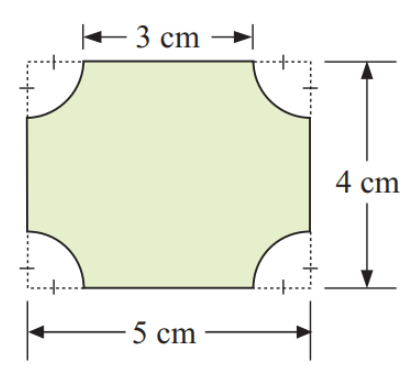
\includegraphics[scale=0.5]{data/Hình/C48_TN_HH}
		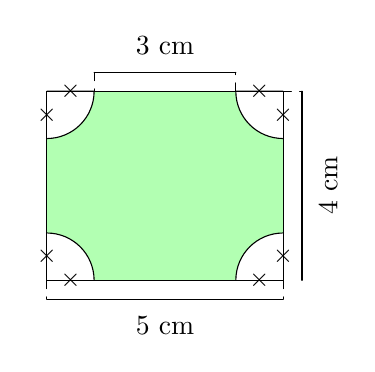
\begin{tikzpicture}[scale=1,line join=round,line cap=round,>=stealth]
		\def\a{0.6} 
		
		
		\path
		(0,0)coordinate(O)
		(90:1*\a)coordinate(A)
		(90:3*\a)coordinate(B)
		(90:4*\a)coordinate(C)
		
		(0:1*\a)coordinate(D)
		(0:4*\a)coordinate(E)
		(0:5*\a)coordinate(F)
		
		(F)++(90:1*\a)coordinate(G)
		(F)++(90:3*\a)coordinate(H)
		(F)++(90:4*\a)coordinate(K)
		
		(C)++(0:1*\a)coordinate(I)
		(C)++(0:4*\a)coordinate(J)
		(C)++(0:5*\a)coordinate(M)
		
		(I)++(90:0.4*\a)coordinate(i)
		(J)++(90:0.4*\a)coordinate(j)
		
		(O)++(-90:0.4*\a)coordinate(o)
		(F)++(-90:0.4*\a)coordinate(f)
		
		(K)++(0:0.4*\a)coordinate(k)
		(F)++(0:0.4*\a)coordinate(f')
	
		;
		
		
		\draw[dashed, fill=green!30] (O)--(C)--(K)--(F)--(O);
		
		\draw [fill=white]  
		(C)--++(0:1*\a) arc (0:-90:1*\a)-- cycle
		(K)--++(180:1*\a) arc (180:270:1*\a)-- cycle
		(O)--++(0:1*\a) arc (0:90:1*\a)-- cycle
		(F)--++(90:1*\a) arc (90:180:1*\a)-- cycle
		
		;  
		
		\fill[white]
		(B)--(C)--(I)--(B)(K)--(H)--(J)--(K)(O)--(A)--(D)--(O)(E)--(G)--(F)--(E);
		
		\draw    
		(A)--(B)--(C)node[midway]{\small $\times$}--(I)node[midway]{\small $\times$}--(J)--(K)node[midway]{\small $\times$}-- (H)node[midway]{\small $\times$}--(G)--(F)node[midway]{\small $\times$}--(E)node[midway]{\small $\times$}-- (D)--(O)node[midway]{\small $\times$}--(A)node[midway]{\small $\times$};
		\draw[dashed](i)--(I) (J)--(j) (O)--(o) (K)--(k) (F)--(f);
		\draw[>=stealth]
		(i) -- (j)node[midway,above, rotate=0,yshift=0.1 cm]{$3$ cm}
		(o) -- (f)node[midway,below, rotate=0,yshift=-0.1 cm]{$5$ cm}
		(k) --(f')node[midway,below, rotate=90,yshift=-0.1 cm]{$4$ cm}
		;
		
		%%%% Hiển thị tên điểm
		%		\foreach \x/\g in {A/-40,O/90,C/90,D/9,B/9,E/9,F/9,G/9,H/9,K/9,I/9,J/9,K/9			}\draw[fill=white](\x)circle(1.5pt)+(\g:.3)node{$\x$};
	\end{tikzpicture}
	}
	
\end{ex}


	
%%=====Câu 49

\begin{ex}\immini[thm]{
	Hãy tính diện tích phần tô đậm, cho biết diện tích đó gần nhất với kết quả nào sau đây:
	
	\choice
	{\True 6,6 cm$^2$}
	{3,6 cm$^2$}
	{4,4 cm$^2$}
	{7,4 cm$^2$}	
	}{
		%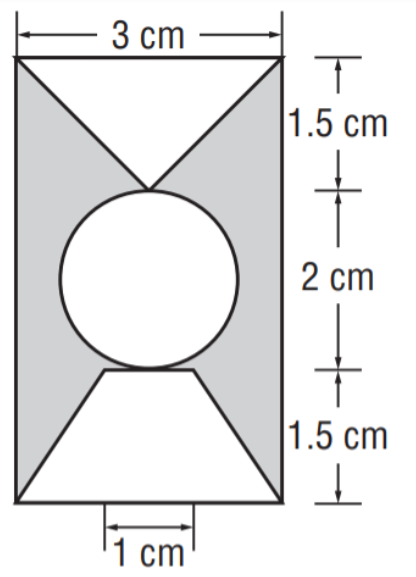
\includegraphics[scale=0.4]{data/Hình/C49_TN_HH}
		\begin{tikzpicture}[scale=1,line join=round,line cap=round,>=stealth]
			\def\a{0.82} 
			
			\path
			(0,0)coordinate(O)
			(0:3*\a)coordinate(A)
			(90:5*\a)coordinate(D)
			(D)++(0:3*\a)coordinate(C)
			
			($(D)!0.5!(C)$) coordinate(b)
			(b)++(-90:1.5*\a)coordinate(B)
			(b)++(-90:2.5*\a)coordinate(E)
			
			($(O)!0.5!(A)$) coordinate(f)
			(f)++(90:1.5*\a)coordinate(g)
			(g)++(0:0.5*\a)coordinate(G)
			(g)++(0:-0.5*\a)coordinate(H)
			%
			(D)++(90:0.4*\a)coordinate(k)
			(C)++(90:0.4*\a)coordinate(f')
			(C)++(0:0.4*\a)coordinate(i)
			(B)++(0:1.9*\a)coordinate(j)
			(g)++(0:1.9*\a)coordinate(o)
			(A)++(0:0.4*\a)coordinate(m)
			(B)++(0:2.1*\a)coordinate(j')
			(g)++(0:2.1*\a)coordinate(o')
			(H)++(-90:1.63*\a)coordinate(p)
			(G)++(-90:1.63*\a)coordinate(q)
			;
			
			\draw[ fill=green!30]
			(O)--(A)--(C)--(D)--(O);
			\draw [fill=white]
			(D)--(B)--(C)--(D)
			(O)--(H)--(G)--(A)
			(E) circle (\a cm)
			; 
			\draw[>=stealth]
			(i) -- (j)node[midway,below , rotate=90,yshift=-0.12 cm]{$1.5$ cm}
			(o) -- (m)node[midway,below, rotate=90,yshift=-0.12 cm]{$1.5$ cm}
			(k) --(f')node[midway,below, rotate=0,yshift=0.55 cm]{$3$ cm}
			(j') --(o')node[midway,below, rotate=90,yshift=-0.12 cm]{$2$ cm}
			(p) --(q)node[midway,below, rotate=0,yshift=-0.12 cm]{$1$ cm}
			;
			\draw[dashed](C)--(i) (B)--(j') (g)--(o')(A)--(m) (D)--(k)(C)--(f') (H)--(p) (G)--(q);
			%%%% Hiển thị tên điểm
		%		\foreach \x/\g in {A/-40,D/90,C/90,O/-130,E/9,B/9,b/9,f/9,G/9,H/9,g/9,k/9,p/9,q/9,j'/9,o'/9,f'/9,i/9,j/9,m/9,o/9	}\draw[fill=white](\x)circle(1.5pt)+(\g:.3)node{$\x$};
		\end{tikzpicture}
	}
		
\end{ex}

\begin{ex}%[6H1B2-4] 
	Bác Hòa uốn một sợi dây thép thành móc treo đồ có dạng hình thang cân với độ dài đáy bé bằng 40 cm, đáy lớn bằng 50 cm cạnh bên bằng 15 cm móc treo dài 10 cm. Hỏi bác Hòa cần bao nhiên mét dây thép? 
	\choice
	{ 130 m}
	{ 1,3 m}
	{\True 130 cm}
	{1,3 cm}
\end{ex}

%%=====Câu 57
\begin{ex}\immini[thm]{
		So sánh diện tích hình thoi và hình chữ nhật bên:
		\choice
		{Diện tích hình thoi lớn hơn}
		{\True Diện tích hình chữ nhật lớn hơn}
		{Diện tích hình chữ nhật gấp 3 lần diện tích hình thoi}
		{ Diện tích hình chữ nhật bằng diện tích hình thoi}
	}{
		\begin{tikzpicture}[scale=1,line width=0.8pt,line join=round,>=stealth]
			\def\a{4} 	\def\b{2.4} 
			\path (0,0) coordinate (A)
			(A)+(-90:\a) coordinate (C)
			(A)+(-\b/2,-\a/2) coordinate (B)
			(B)+(0:\b) coordinate (D)
			;
			\draw[latex-] (B)++(0:0.5)--++(120:0.5*\b)node[above]{\small 12 cm} ;
			\draw[latex-] (C)++(90:1)--++(-160:1.5)node[below left]{\small 20 cm} ;
			\draw (A)--(B)--(C)--(D)--(A)--(C) (B)--(D);
			\draw (3,0)--++(0:\b)node[above,midway]{\small 12 cm}--++(-90:\a)--++(180:\b)--cycle node[sloped,above,midway]{\small 20 cm};
		\end{tikzpicture}
	}
	
\end{ex}


\begin{ex}
	Một thửa ruộng hình chữ nhật có chiều dài 	là 24 m, chiều rộng 18 m. Trên thửa ruộng đó, mỗi 
	mét vuông thu hoạch được 5 kg rau. Hỏi cả thửa 	ruộng đó thu hoạch được bao nhiêu ki – lô – gam 
	rau? 
	
	\choice
	{432 kg}
	{\True 2160 kg}
	{518 kg}
	{1080 kg}
	
\end{ex}

\begin{ex}%[6H1B2-4] 
	Một nền nhà hình chữ nhật có chiều dài 20 m và chiều rộng bằng $\frac{1}{4}$ chiều dài. Người ta muốn lát gạch hình vuông cạnh 5 dm lên nền nhà đó nên đã mua gạch với tổng số tiền là $36\,800\,000$ đồng (giả sử khoảng cách giữa hai viên gạch kề nhau là không đáng kể). Hỏi giá của một viên gạch là bao nhiêu?
	\choice
	{ $90\,000$ đồng}
	{ $91\,000$ đồng)}
	{\True $92\,000$ đồng}
	{$93\,000$ đồng}
\end{ex}

%%=====Câu 55
\begin{ex}\immini[thm]{
	Tính diện tích hình bên:
	\choice
	{180 m}
	{1550 m}
	{\True 1550 m$^ 2$}
	{ 180 m$^2$}	
	}{\begin{tikzpicture}[scale=1,line width=0.8pt,line join=round,>=stealth]
		\def\sc{15} 
		\path (0,0) coordinate (A)
		(A)+(15/\sc,20/\sc) coordinate (B)
		(B)+(40/\sc,30/\sc) coordinate (C)
		(B)+(0:40/\sc) coordinate (D)
		(A)+(0:55/\sc) coordinate (E)
		;
		\draw[latex-latex,dashed] (A)++(180:0.3)--++(90:20/\sc)node[midway,left]{\small 20 cm} ;
		\draw[latex-latex,dashed] (C)++(0:0.6)--++(-90:50/\sc)node[midway,right]{\small 50 cm} ;
		\draw[latex-latex,dashed] (C)++(90:0.3)--++(180:40/\sc)node[midway,above]{\small 40 cm} ;
		\draw (A)--(B)node[midway,above,sloped]{\small 25 cm}
		--(C)node[midway,above,sloped]{\small 50 cm}
		--(E)--(A)node[midway,below]{\small 55 cm} (B)--(D);
		\draw[dashed] (B)--++(180:15/\sc+0.3)
			(B)--++(90:30/\sc+0.3);
		\foreach \x/ \goc in {A/-90,B/135,C/0,D/0,E/-45}  \fill (\x) circle (1.5pt)	
				($(\x)+(\goc:3mm)$) node {$\x$};
	\end{tikzpicture}	
	}
\end{ex}



%%=====Câu 59
\begin{ex}\immini[thm]{
	Cho hình chữ nhật $ABFE$ và hình thoi $ABCD$, biết $CD=5$ cm và $AE=2$ cm. Diện tích của hình chữ nhật $ABFE$ bằng:
	\choice
	{14 cm$^2$}
	{7 cm$^2$}
	{\True 10 cm$^2$}
	{5 cm$^2$}	
	}{
	\begin{tikzpicture}[scale=1,line width=0.8pt,line join=round,>=stealth]
		\def\a{2.5} 	\def\b{1} 	\def\g{20} 
		\path (0,0) coordinate (A)
		(A)+(\g-180:\a) coordinate (B)
		(B)+(-\g:\a) coordinate (C)
		(C)+(\g:\a) coordinate (D)
		(A)+(90+\g:\b) coordinate (E)
		(E)+(B) coordinate (F)
		;
		\draw[latex-latex] (A)++(\g:0.3)--++(90+\g:\b)node[midway,right]{\small 2 cm} ;
		\draw[latex-latex] (C)++(\g-90:0.3)--++(\g:\a)node[midway,below,sloped]{\small 5 cm} ;
		\draw (A)--(B)--(C)--(D)--(A)--(E)--(F)--(B);
		\foreach \x/ \goc in {A/160,B/200,C/-120,D/30,E/90,F/160}  \fill (\x) circle (1.5pt)	
		($(\x)+(\goc:3mm)$) node {$\x$};
	\end{tikzpicture}
	}
	
\end{ex}


  %2	
		\Closesolutionfile{ans}


          %------------------------%
\part{ĐÁP SỐ ĐỀ ÔN TẬP}
\setcounter{section}{0} 
\newcommand{\dsection}[1]{%
	\section{ĐỀ SỐ \thesection}%
	\input{ans/ansD#1}%
} 
\dsection{1}
\dsection{2}
\dsection{3}
\dsection{4}
\dsection{5}
\dsection{6}
\dsection{7}
\dsection{8}
\dsection{9}
\dsection{10}
\dsection{11}
\dsection{12}
\dsection{13}
\dsection{14}
\dsection{15}
\dsection{16}
\dsection{17}
\dsection{18}
\dsection{19}
\dsection{20} 
\dsection{21}
\dsection{22}
\dsection{23}
\dsection{24}
\dsection{25}
    \newpage
%       ===== PHẦN TRẮC NGHIỆM =====
     \part{ĐÁP SỐ TRẮC NGHIỆM}
     \setcounter{section}{0} 
        \subsection{PHẦN ĐẠI SỐ}
       \inputansbox{10}{ans/TN-DS}
       \subsection{PHẦN HÌNH HỌC}
       \inputansbox{10}{ans/TN-HH} 
      
       
        
\end{document}